% $Author: stef $
% $Date: 2008-04-04 17:14:31 +0200 (Fri, 04 Apr 2008) $
% $Revision: 318 $
%=================================================================
\ifx\wholebook\relax\else
% --------------------------------------------
% Lulu:
    \documentclass[a4paper,10pt,twoside]{book}
    \usepackage[
        papersize={6in,9in},
        hmargin={.75in,.75in},
        vmargin={.75in,1in},
        ignoreheadfoot
    ]{geometry}
    % $Author$ Martial
% $Date$ Wed Oct 10 13:34:55 CEST 2007
% $Revision$ source: SBE 12715 
% Last Changed Date: 2007-10-08 21:32:45 +0200 (Mon, 08 Oct 2007)
%=============================================================
% NB: documentclass must be set in main document.
% Allows book to be generated in multiple formats.
%=============================================================
%:Packages
%\usepackage[french]{babel}
\usepackage[T1]{fontenc}  %%%%%% really important to get the code directly in the text!
\usepackage{lmodern}
%\usepackage[scaled=0.85]{bookmanx} % needs another scale factor if used with \renewcommand{\sfdefault}{cmbr}
\usepackage{palatino}
%\usepackage[sc]{mathpazo}
%\linespread{1.05}
\usepackage[scaled=0.85]{helvet}
\usepackage{microtype}
\usepackage{graphicx}
\usepackage{theorem}
\usepackage[utf8]{inputenc}
% ON: pdfsync breaks the use of p{width} for tabular columns!
\ifdefined\usepdfsync\usepackage{pdfsync}\fi % Requires texlive 2007
%=============================================================
%:More packages
%Stef should check which ones are used!
%\usepackage{picinpar}
%\usepackage{layout}
%\usepackage{color}
%\definecolor{stefgris}{rgb}{0.85,0.85,0.85}
%\usepackage{enum}
%\usepackage{a4wide}
% \usepackage{fancyhdr}
\usepackage{ifthen}
\usepackage{float}
\usepackage{longtable}
\usepackage{makeidx}
\usepackage[nottoc]{tocbibind}
\usepackage{multicol}
\usepackage{booktabs}	% book-style tables
\usepackage{topcapt}	% enables \topcaption
\usepackage{multirow}
\usepackage{tabularx}
%\usepackage[bottom]{footmisc}
\usepackage{xspace}
\usepackage{alltt}
\usepackage{amssymb,textcomp}
\usepackage[usenames,dvipsnames]{color}
\usepackage{colortbl}
\usepackage[hang]{subfigure}\makeatletter\def\p@subfigure{\thefigure\,}\makeatother
\usepackage{rotating}
\usepackage{enumitem}	% apb: allows more control over tags in enumerations
\usepackage{verbatim}     % for comment environment
\usepackage{varioref}	% for page references that work
\labelformat{footnote}{\thechapter--#1} % to distinguish citations from jurabib
\usepackage{needspace}
\usepackage{isodateo} % enable \isodate
\usepackage[newparttoc]{titlesec}
\usepackage{titletoc}
\usepackage{eurosym}
\usepackage{wrapfig}

\usepackage[
	super,
	citefull=first,
	authorformat={allreversed,and},
	titleformat={commasep,italic}
]{jurabib} % citations as footnotes
\usepackage[
	colorlinks=true,
	linkcolor=black,
	urlcolor=black,
	citecolor=black
]{hyperref}   % should come last

%=============================================================
%:URL style
\makeatletter

\def\url@leostyle{%
  \@ifundefined{selectfont}{\def\UrlFont{\sf}}{\def\UrlFont{\sffamily}}}
% ajouter par Martial pour \traduit (met une dague dans les \doublebox
\def\thempfootnote{\fnsymbol{mpfootnote}}

\makeatother
% Now actually use the newly defined style.
\urlstyle{leo}
%=============================================================
%:Booleans
\newboolean{lulu}
\setboolean{lulu}{false}
\newcommand{\ifluluelse}[2]{\ifthenelse{\boolean{lulu}}{#1}{#2}}
%=============================================================
%:Names
\newcommand{\SUnit}{SUnit\xspace}
\newcommand{\sunit}{SUnit\xspace}
\newcommand{\xUnit}{$x$Unit\xspace}
\newcommand{\JUnit}{JUnit\xspace}
%\newcommand{\XP}{eXtreme Programming\xspace}
\newcommand{\st}{Smalltalk\xspace}
\newcommand{\Squeak}{Squeak\xspace}
\newcommand{\sq}{Squeak\xspace}
\newcommand{\sqmap}{SqueakMap\xspace}
\newcommand{\squeak}{Squeak\xspace}
%\newcommand{\sbe}{\url{scg.unibe.ch/SBE}\xspace}
%\newcommand{\sbe}{\url{squeakbyexample.org}\xspace}
\newcommand{\sbe}{\url{SqueakByExample.org}\xspace}
% squeak-fr: adresse de la version francaise
\newcommand{\spe}{\url{SqueakByExample.org/fr}\xspace}
\newcommand{\sba}{\url{SquareBracketAssociates.org}\xspace}

% squeak-fr: ajout de la \squeakdev pour eviter les problemes de
% changements d'url rencontres dans la VO:
\newcommand{\squeakdev}{\url{www.squeaksource.com/ImageForDevelopers}\xspace} %ou
%\newcommand{\squeakdev}{\url{squeak.ofset.org/squeak-dev}\xspace}

%=============================================================
%:Editorial comment macros
\newcommand{\nnbb}[2]{
    \fbox{\bfseries\sffamily\scriptsize#1}
    {\sf\small$\blacktriangleright$\textit{#2}$\blacktriangleleft$}
   }
\newcommand{\ab}[1]{\nnbb{Andrew}{#1}}
\newcommand{\sd}[1]{\nnbb{St\'{e}f}{#1}}
\newcommand{\md}[1]{\nnbb{Marcus}{#1}}
\newcommand{\on}[1]{\nnbb{Oscar}{#1}}
\newcommand{\damien}[1]{\nnbb{Damien}{#1}}
\newcommand{\lr}[1]{\nnbb{Lukas}{#1}}
\newcommand{\orla}[1]{\nnbb{Orla}{#1}}
%\newcommand{\here}{\nnbb{CONTINUE}{HERE}}
\newcommand{\here}{\nnbb{CONTINUE}{ICI}}

%=============================================================
%:Abbreviation macros
\newcommand{\ie}{\emph{c-\`a-d.}\xspace}
\newcommand{\cad}{\emph{c-\`a-d.}\xspace}
%\newcommand{\eg}{\emph{e.g.},\xspace}
\newcommand{\eg}{\emph{par ex.},\xspace}
\newcommand{\parex}{\emph{par ex.},\xspace}
\newcommand{\etc}{etc\xspace}
%=============================================================
%:Cross reference macros

% [squeak-fr] martial: remarquez les articles devant les noms
\newcommand{\charef}[1]{le chapitre~\ref{cha:#1}\xspace}
% note de martial: utilise dans chapitre Syntax.tex: a redefinir
\newcommand{\charefs}[2]{les chapitres~\ref{cha:#1} et \ref{cha:#2}\xspace}
\newcommand{\secref}[1]{la section~\ref{sec:#1}\xspace}
\newcommand{\figref}[1]{la figure~\ref{fig:#1}\xspace}
\newcommand{\Figref}[1]{La figure~\ref{fig:#1}\xspace}
\newcommand{\appref}[1]{l'annexe~\ref{app:#1}\xspace}
\newcommand{\tabref}[1]{la table~\ref{tab:#1}\xspace}
% defini pour le chapitre Messages.tex
\newcommand{\Tabref}[1]{La table~\ref{tab:#1}\xspace}

% APB: I removed trailing \xspace commands from these macros because
% \xspace mostly doesn't work.  If you want a space after your
% references, type one!
% ON: xspace has always worked just fine for me!  Please leave them in.
%
\newcommand{\ruleref}[1]{\ref{rule:#1}\xspace}
%
\newcommand{\egref}[1]{exemple~\ref{eg:#1}\xspace}
\newcommand{\Egref}[1]{Exemple~\ref{eg:#1}\xspace}
%
\newcommand{\scrref}[1]{script~\ref{scr:#1}\xspace}
\newcommand{\Scrref}[1]{Script~\ref{scr:#1}\xspace}
% t = the
\newcommand{\tscrref}[1]{le script~\ref{scr:#1}\xspace}
\newcommand{\Tscrref}[1]{Le script~\ref{scr:#1}\xspace}
%
\newcommand{\mthref}[1]{m\'ethode~\ref{mth:#1}\xspace}
\newcommand{\mthsref}[1]{m\'ethodes~\ref{mth:#1}\xspace}
\newcommand{\Mthref}[1]{M\'ethode~\ref{mth:#1}\xspace}
\newcommand{\tmthref}[1]{la m\'ethode~\ref{mth:#1}\xspace}
\newcommand{\Tmthref}[1]{La m\'ethode~\ref{mth:#1}\xspace}
%
\newcommand{\clsref}[1]{classe~\ref{cls:#1}\xspace}
\newcommand{\tclsref}[1]{la classe~\ref{cls:#1}\xspace}
\newcommand{\Tclsref}[1]{La classe~\ref{cls:#1}\xspace}
%=============================================================
%:Menu item macro
% for menu items, so we can change our minds on how to print them! (apb)
\definecolor{lightgray}{gray}{0.89}
\newcommand{\menu}[1]{{%
	\setlength{\fboxsep}{0pt}%
	\colorbox{lightgray}{{{\upshape\sffamily\strut \,#1\,}}}}}
% \newcommand{\menu}[1]{{%
% 	\fontfamily{lmr}\selectfont
% 	\upshape\textlangle{\sffamily #1}\textrangle}}
% For submenu items:
\newcommand{\go}{\,$\triangleright$\,}
% \newcommand{\go}{\,$\blacktriangleright$\,}
% For keyboard shortcuts:
%\newcommand{\short}[1]{\mbox{$\langle${\sc CMD}$\rangle$-#1}\xspace}
\newcommand{\short}[1]{\mbox{{\sc cmd}\hspace{0.08em}--\hspace{0.09em}#1}\xspace}
% For buttons:
\newcommand{\button}[1]{{%
	\setlength{\fboxsep}{0pt}%
	\fbox{{\upshape\sffamily\strut \,#1\,}}}}
\newcommand{\toolsflap}{l'onglet \textit{Tools}\xspace}
%=============================================================
%:Reader cues (do this)
%
% Indicate something the reader should try out.
\newcommand{\dothisicon}{\raisebox{-.5ex}{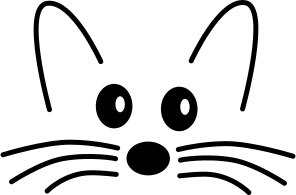
\includegraphics[width=1.4em]{squeak-logo}}}
\newcommand{\dothis}[1]{%
	\medskip
	\noindent\dothisicon
	\ifx#1\empty\else\quad\emph{#1}\fi
	\par\smallskip\nopagebreak}
% NB: To use this in an individual chapter, you must set:
%\graphicspath{{figures/} {../figures/}}
% at the head of the chapter.  Don't forget the final /
%=============================================================
%:Reader hints (hint)
%
% Indicates a non-obvious consequence 
\newcommand{\hint}[1]{\vspace{1ex}\noindent\fbox{\textsc{Astuce}} \emph{#1}}
%=================================================================
% graphics for Morphic handles
\newcommand{\grabHandle}{\raisebox{-0.2ex}{
\includegraphics[width=1em]{blackHandle}}}
\newcommand{\moveHandle}{\raisebox{-0.2ex}{
\includegraphics[width=1em]{moveHandle}}}
\newcommand{\debugHandle}{\raisebox{-0.2ex}{
\includegraphics[width=1em]{debugHandle}}}
% squeak-fr (added for Morphic handles)
\newcommand{\rotateHandle}{\raisebox{-0.2ex}{
\includegraphics[width=1em]{rotateHandle}}}
\newcommand{\viewerHandle}{\raisebox{-0.2ex}{
\includegraphics[width=1em]{viewerHandle}}}
% squeak-fr (add cloverHandle to use \clover in QuickTour.tex as alias
% todo 

%=============================================================
%:Highlighting Important stuff (doublebox)
%
% From Seaside book ...
\newsavebox{\SavedText}
\newlength{\InnerBoxRule}\setlength{\InnerBoxRule}{.75\fboxrule}
\newlength{\OuterBoxRule}\setlength{\OuterBoxRule}{1.5\fboxrule}
\newlength{\BoxSeparation}\setlength{\BoxSeparation}{1.5\fboxrule}
\addtolength{\BoxSeparation}{.5pt}
\newlength{\SaveBoxSep}\setlength{\SaveBoxSep}{2\fboxsep}
%
\newenvironment{doublebox}{\begin{lrbox}{\SavedText}
    \begin{minipage}{.75\textwidth}}
    {\end{minipage}\end{lrbox}\begin{center}
    \setlength{\fboxsep}{\BoxSeparation}\setlength{\fboxrule}{\OuterBoxRule}
    \fbox{\setlength{\fboxsep}{\SaveBoxSep}\setlength{\fboxrule}{\InnerBoxRule}%
      \fbox{\usebox{\SavedText}}}
  \end{center}}
% Use this:
%\newcommand{\important}[1]{\begin{doublebox}#1\end{doublebox}}


\newcommand{\important}[1]{
\noindent\rule{\textwidth}{2pt}\par
\textbf{Important!} #1 \par
\noindent\rule{\textwidth}{2pt}}

\newcommand{\note}[1]{
\noindent\rule{\textwidth}{2pt}\par
\noindent\textbf{Note} #1\par
\noindent\rule{\textwidth}{2pt}}

%=============================================================
%:Section depth
\setcounter{secnumdepth}{2}
%% for this to happen start the file with
%\ifx\wholebook\relax\else
%% $Author$ Martial
% $Date$ Wed Oct 10 13:34:55 CEST 2007
% $Revision$ source: SBE 12715 
% Last Changed Date: 2007-10-08 21:32:45 +0200 (Mon, 08 Oct 2007)
%=============================================================
% NB: documentclass must be set in main document.
% Allows book to be generated in multiple formats.
%=============================================================
%:Packages
%\usepackage[french]{babel}
\usepackage[T1]{fontenc}  %%%%%% really important to get the code directly in the text!
\usepackage{lmodern}
%\usepackage[scaled=0.85]{bookmanx} % needs another scale factor if used with \renewcommand{\sfdefault}{cmbr}
\usepackage{palatino}
%\usepackage[sc]{mathpazo}
%\linespread{1.05}
\usepackage[scaled=0.85]{helvet}
\usepackage{microtype}
\usepackage{graphicx}
\usepackage{theorem}
\usepackage[utf8]{inputenc}
% ON: pdfsync breaks the use of p{width} for tabular columns!
\ifdefined\usepdfsync\usepackage{pdfsync}\fi % Requires texlive 2007
%=============================================================
%:More packages
%Stef should check which ones are used!
%\usepackage{picinpar}
%\usepackage{layout}
%\usepackage{color}
%\definecolor{stefgris}{rgb}{0.85,0.85,0.85}
%\usepackage{enum}
%\usepackage{a4wide}
% \usepackage{fancyhdr}
\usepackage{ifthen}
\usepackage{float}
\usepackage{longtable}
\usepackage{makeidx}
\usepackage[nottoc]{tocbibind}
\usepackage{multicol}
\usepackage{booktabs}	% book-style tables
\usepackage{topcapt}	% enables \topcaption
\usepackage{multirow}
\usepackage{tabularx}
%\usepackage[bottom]{footmisc}
\usepackage{xspace}
\usepackage{alltt}
\usepackage{amssymb,textcomp}
\usepackage[usenames,dvipsnames]{color}
\usepackage{colortbl}
\usepackage[hang]{subfigure}\makeatletter\def\p@subfigure{\thefigure\,}\makeatother
\usepackage{rotating}
\usepackage{enumitem}	% apb: allows more control over tags in enumerations
\usepackage{verbatim}     % for comment environment
\usepackage{varioref}	% for page references that work
\labelformat{footnote}{\thechapter--#1} % to distinguish citations from jurabib
\usepackage{needspace}
\usepackage{isodateo} % enable \isodate
\usepackage[newparttoc]{titlesec}
\usepackage{titletoc}
\usepackage{eurosym}
\usepackage{wrapfig}

\usepackage[
	super,
	citefull=first,
	authorformat={allreversed,and},
	titleformat={commasep,italic}
]{jurabib} % citations as footnotes
\usepackage[
	colorlinks=true,
	linkcolor=black,
	urlcolor=black,
	citecolor=black
]{hyperref}   % should come last

%=============================================================
%:URL style
\makeatletter

\def\url@leostyle{%
  \@ifundefined{selectfont}{\def\UrlFont{\sf}}{\def\UrlFont{\sffamily}}}
% ajouter par Martial pour \traduit (met une dague dans les \doublebox
\def\thempfootnote{\fnsymbol{mpfootnote}}

\makeatother
% Now actually use the newly defined style.
\urlstyle{leo}
%=============================================================
%:Booleans
\newboolean{lulu}
\setboolean{lulu}{false}
\newcommand{\ifluluelse}[2]{\ifthenelse{\boolean{lulu}}{#1}{#2}}
%=============================================================
%:Names
\newcommand{\SUnit}{SUnit\xspace}
\newcommand{\sunit}{SUnit\xspace}
\newcommand{\xUnit}{$x$Unit\xspace}
\newcommand{\JUnit}{JUnit\xspace}
%\newcommand{\XP}{eXtreme Programming\xspace}
\newcommand{\st}{Smalltalk\xspace}
\newcommand{\Squeak}{Squeak\xspace}
\newcommand{\sq}{Squeak\xspace}
\newcommand{\sqmap}{SqueakMap\xspace}
\newcommand{\squeak}{Squeak\xspace}
%\newcommand{\sbe}{\url{scg.unibe.ch/SBE}\xspace}
%\newcommand{\sbe}{\url{squeakbyexample.org}\xspace}
\newcommand{\sbe}{\url{SqueakByExample.org}\xspace}
% squeak-fr: adresse de la version francaise
\newcommand{\spe}{\url{SqueakByExample.org/fr}\xspace}
\newcommand{\sba}{\url{SquareBracketAssociates.org}\xspace}

% squeak-fr: ajout de la \squeakdev pour eviter les problemes de
% changements d'url rencontres dans la VO:
\newcommand{\squeakdev}{\url{www.squeaksource.com/ImageForDevelopers}\xspace} %ou
%\newcommand{\squeakdev}{\url{squeak.ofset.org/squeak-dev}\xspace}

%=============================================================
%:Editorial comment macros
\newcommand{\nnbb}[2]{
    \fbox{\bfseries\sffamily\scriptsize#1}
    {\sf\small$\blacktriangleright$\textit{#2}$\blacktriangleleft$}
   }
\newcommand{\ab}[1]{\nnbb{Andrew}{#1}}
\newcommand{\sd}[1]{\nnbb{St\'{e}f}{#1}}
\newcommand{\md}[1]{\nnbb{Marcus}{#1}}
\newcommand{\on}[1]{\nnbb{Oscar}{#1}}
\newcommand{\damien}[1]{\nnbb{Damien}{#1}}
\newcommand{\lr}[1]{\nnbb{Lukas}{#1}}
\newcommand{\orla}[1]{\nnbb{Orla}{#1}}
%\newcommand{\here}{\nnbb{CONTINUE}{HERE}}
\newcommand{\here}{\nnbb{CONTINUE}{ICI}}

%=============================================================
%:Abbreviation macros
\newcommand{\ie}{\emph{c-\`a-d.}\xspace}
\newcommand{\cad}{\emph{c-\`a-d.}\xspace}
%\newcommand{\eg}{\emph{e.g.},\xspace}
\newcommand{\eg}{\emph{par ex.},\xspace}
\newcommand{\parex}{\emph{par ex.},\xspace}
\newcommand{\etc}{etc\xspace}
%=============================================================
%:Cross reference macros

% [squeak-fr] martial: remarquez les articles devant les noms
\newcommand{\charef}[1]{le chapitre~\ref{cha:#1}\xspace}
% note de martial: utilise dans chapitre Syntax.tex: a redefinir
\newcommand{\charefs}[2]{les chapitres~\ref{cha:#1} et \ref{cha:#2}\xspace}
\newcommand{\secref}[1]{la section~\ref{sec:#1}\xspace}
\newcommand{\figref}[1]{la figure~\ref{fig:#1}\xspace}
\newcommand{\Figref}[1]{La figure~\ref{fig:#1}\xspace}
\newcommand{\appref}[1]{l'annexe~\ref{app:#1}\xspace}
\newcommand{\tabref}[1]{la table~\ref{tab:#1}\xspace}
% defini pour le chapitre Messages.tex
\newcommand{\Tabref}[1]{La table~\ref{tab:#1}\xspace}

% APB: I removed trailing \xspace commands from these macros because
% \xspace mostly doesn't work.  If you want a space after your
% references, type one!
% ON: xspace has always worked just fine for me!  Please leave them in.
%
\newcommand{\ruleref}[1]{\ref{rule:#1}\xspace}
%
\newcommand{\egref}[1]{exemple~\ref{eg:#1}\xspace}
\newcommand{\Egref}[1]{Exemple~\ref{eg:#1}\xspace}
%
\newcommand{\scrref}[1]{script~\ref{scr:#1}\xspace}
\newcommand{\Scrref}[1]{Script~\ref{scr:#1}\xspace}
% t = the
\newcommand{\tscrref}[1]{le script~\ref{scr:#1}\xspace}
\newcommand{\Tscrref}[1]{Le script~\ref{scr:#1}\xspace}
%
\newcommand{\mthref}[1]{m\'ethode~\ref{mth:#1}\xspace}
\newcommand{\mthsref}[1]{m\'ethodes~\ref{mth:#1}\xspace}
\newcommand{\Mthref}[1]{M\'ethode~\ref{mth:#1}\xspace}
\newcommand{\tmthref}[1]{la m\'ethode~\ref{mth:#1}\xspace}
\newcommand{\Tmthref}[1]{La m\'ethode~\ref{mth:#1}\xspace}
%
\newcommand{\clsref}[1]{classe~\ref{cls:#1}\xspace}
\newcommand{\tclsref}[1]{la classe~\ref{cls:#1}\xspace}
\newcommand{\Tclsref}[1]{La classe~\ref{cls:#1}\xspace}
%=============================================================
%:Menu item macro
% for menu items, so we can change our minds on how to print them! (apb)
\definecolor{lightgray}{gray}{0.89}
\newcommand{\menu}[1]{{%
	\setlength{\fboxsep}{0pt}%
	\colorbox{lightgray}{{{\upshape\sffamily\strut \,#1\,}}}}}
% \newcommand{\menu}[1]{{%
% 	\fontfamily{lmr}\selectfont
% 	\upshape\textlangle{\sffamily #1}\textrangle}}
% For submenu items:
\newcommand{\go}{\,$\triangleright$\,}
% \newcommand{\go}{\,$\blacktriangleright$\,}
% For keyboard shortcuts:
%\newcommand{\short}[1]{\mbox{$\langle${\sc CMD}$\rangle$-#1}\xspace}
\newcommand{\short}[1]{\mbox{{\sc cmd}\hspace{0.08em}--\hspace{0.09em}#1}\xspace}
% For buttons:
\newcommand{\button}[1]{{%
	\setlength{\fboxsep}{0pt}%
	\fbox{{\upshape\sffamily\strut \,#1\,}}}}
\newcommand{\toolsflap}{l'onglet \textit{Tools}\xspace}
%=============================================================
%:Reader cues (do this)
%
% Indicate something the reader should try out.
\newcommand{\dothisicon}{\raisebox{-.5ex}{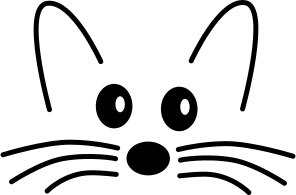
\includegraphics[width=1.4em]{squeak-logo}}}
\newcommand{\dothis}[1]{%
	\medskip
	\noindent\dothisicon
	\ifx#1\empty\else\quad\emph{#1}\fi
	\par\smallskip\nopagebreak}
% NB: To use this in an individual chapter, you must set:
%\graphicspath{{figures/} {../figures/}}
% at the head of the chapter.  Don't forget the final /
%=============================================================
%:Reader hints (hint)
%
% Indicates a non-obvious consequence 
\newcommand{\hint}[1]{\vspace{1ex}\noindent\fbox{\textsc{Astuce}} \emph{#1}}
%=================================================================
% graphics for Morphic handles
\newcommand{\grabHandle}{\raisebox{-0.2ex}{
\includegraphics[width=1em]{blackHandle}}}
\newcommand{\moveHandle}{\raisebox{-0.2ex}{
\includegraphics[width=1em]{moveHandle}}}
\newcommand{\debugHandle}{\raisebox{-0.2ex}{
\includegraphics[width=1em]{debugHandle}}}
% squeak-fr (added for Morphic handles)
\newcommand{\rotateHandle}{\raisebox{-0.2ex}{
\includegraphics[width=1em]{rotateHandle}}}
\newcommand{\viewerHandle}{\raisebox{-0.2ex}{
\includegraphics[width=1em]{viewerHandle}}}
% squeak-fr (add cloverHandle to use \clover in QuickTour.tex as alias
% todo 

%=============================================================
%:Highlighting Important stuff (doublebox)
%
% From Seaside book ...
\newsavebox{\SavedText}
\newlength{\InnerBoxRule}\setlength{\InnerBoxRule}{.75\fboxrule}
\newlength{\OuterBoxRule}\setlength{\OuterBoxRule}{1.5\fboxrule}
\newlength{\BoxSeparation}\setlength{\BoxSeparation}{1.5\fboxrule}
\addtolength{\BoxSeparation}{.5pt}
\newlength{\SaveBoxSep}\setlength{\SaveBoxSep}{2\fboxsep}
%
\newenvironment{doublebox}{\begin{lrbox}{\SavedText}
    \begin{minipage}{.75\textwidth}}
    {\end{minipage}\end{lrbox}\begin{center}
    \setlength{\fboxsep}{\BoxSeparation}\setlength{\fboxrule}{\OuterBoxRule}
    \fbox{\setlength{\fboxsep}{\SaveBoxSep}\setlength{\fboxrule}{\InnerBoxRule}%
      \fbox{\usebox{\SavedText}}}
  \end{center}}
% Use this:
%\newcommand{\important}[1]{\begin{doublebox}#1\end{doublebox}}


\newcommand{\important}[1]{
\noindent\rule{\textwidth}{2pt}\par
\textbf{Important!} #1 \par
\noindent\rule{\textwidth}{2pt}}

\newcommand{\note}[1]{
\noindent\rule{\textwidth}{2pt}\par
\noindent\textbf{Note} #1\par
\noindent\rule{\textwidth}{2pt}}

%=============================================================
%:Section depth
\setcounter{secnumdepth}{2}
%% for this to happen start the file with
%\ifx\wholebook\relax\else
%% $Author$ Martial
% $Date$ Wed Oct 10 13:34:55 CEST 2007
% $Revision$ source: SBE 12715 
% Last Changed Date: 2007-10-08 21:32:45 +0200 (Mon, 08 Oct 2007)
%=============================================================
% NB: documentclass must be set in main document.
% Allows book to be generated in multiple formats.
%=============================================================
%:Packages
%\usepackage[french]{babel}
\usepackage[T1]{fontenc}  %%%%%% really important to get the code directly in the text!
\usepackage{lmodern}
%\usepackage[scaled=0.85]{bookmanx} % needs another scale factor if used with \renewcommand{\sfdefault}{cmbr}
\usepackage{palatino}
%\usepackage[sc]{mathpazo}
%\linespread{1.05}
\usepackage[scaled=0.85]{helvet}
\usepackage{microtype}
\usepackage{graphicx}
\usepackage{theorem}
\usepackage[utf8]{inputenc}
% ON: pdfsync breaks the use of p{width} for tabular columns!
\ifdefined\usepdfsync\usepackage{pdfsync}\fi % Requires texlive 2007
%=============================================================
%:More packages
%Stef should check which ones are used!
%\usepackage{picinpar}
%\usepackage{layout}
%\usepackage{color}
%\definecolor{stefgris}{rgb}{0.85,0.85,0.85}
%\usepackage{enum}
%\usepackage{a4wide}
% \usepackage{fancyhdr}
\usepackage{ifthen}
\usepackage{float}
\usepackage{longtable}
\usepackage{makeidx}
\usepackage[nottoc]{tocbibind}
\usepackage{multicol}
\usepackage{booktabs}	% book-style tables
\usepackage{topcapt}	% enables \topcaption
\usepackage{multirow}
\usepackage{tabularx}
%\usepackage[bottom]{footmisc}
\usepackage{xspace}
\usepackage{alltt}
\usepackage{amssymb,textcomp}
\usepackage[usenames,dvipsnames]{color}
\usepackage{colortbl}
\usepackage[hang]{subfigure}\makeatletter\def\p@subfigure{\thefigure\,}\makeatother
\usepackage{rotating}
\usepackage{enumitem}	% apb: allows more control over tags in enumerations
\usepackage{verbatim}     % for comment environment
\usepackage{varioref}	% for page references that work
\labelformat{footnote}{\thechapter--#1} % to distinguish citations from jurabib
\usepackage{needspace}
\usepackage{isodateo} % enable \isodate
\usepackage[newparttoc]{titlesec}
\usepackage{titletoc}
\usepackage{eurosym}
\usepackage{wrapfig}

\usepackage[
	super,
	citefull=first,
	authorformat={allreversed,and},
	titleformat={commasep,italic}
]{jurabib} % citations as footnotes
\usepackage[
	colorlinks=true,
	linkcolor=black,
	urlcolor=black,
	citecolor=black
]{hyperref}   % should come last

%=============================================================
%:URL style
\makeatletter

\def\url@leostyle{%
  \@ifundefined{selectfont}{\def\UrlFont{\sf}}{\def\UrlFont{\sffamily}}}
% ajouter par Martial pour \traduit (met une dague dans les \doublebox
\def\thempfootnote{\fnsymbol{mpfootnote}}

\makeatother
% Now actually use the newly defined style.
\urlstyle{leo}
%=============================================================
%:Booleans
\newboolean{lulu}
\setboolean{lulu}{false}
\newcommand{\ifluluelse}[2]{\ifthenelse{\boolean{lulu}}{#1}{#2}}
%=============================================================
%:Names
\newcommand{\SUnit}{SUnit\xspace}
\newcommand{\sunit}{SUnit\xspace}
\newcommand{\xUnit}{$x$Unit\xspace}
\newcommand{\JUnit}{JUnit\xspace}
%\newcommand{\XP}{eXtreme Programming\xspace}
\newcommand{\st}{Smalltalk\xspace}
\newcommand{\Squeak}{Squeak\xspace}
\newcommand{\sq}{Squeak\xspace}
\newcommand{\sqmap}{SqueakMap\xspace}
\newcommand{\squeak}{Squeak\xspace}
%\newcommand{\sbe}{\url{scg.unibe.ch/SBE}\xspace}
%\newcommand{\sbe}{\url{squeakbyexample.org}\xspace}
\newcommand{\sbe}{\url{SqueakByExample.org}\xspace}
% squeak-fr: adresse de la version francaise
\newcommand{\spe}{\url{SqueakByExample.org/fr}\xspace}
\newcommand{\sba}{\url{SquareBracketAssociates.org}\xspace}

% squeak-fr: ajout de la \squeakdev pour eviter les problemes de
% changements d'url rencontres dans la VO:
\newcommand{\squeakdev}{\url{www.squeaksource.com/ImageForDevelopers}\xspace} %ou
%\newcommand{\squeakdev}{\url{squeak.ofset.org/squeak-dev}\xspace}

%=============================================================
%:Editorial comment macros
\newcommand{\nnbb}[2]{
    \fbox{\bfseries\sffamily\scriptsize#1}
    {\sf\small$\blacktriangleright$\textit{#2}$\blacktriangleleft$}
   }
\newcommand{\ab}[1]{\nnbb{Andrew}{#1}}
\newcommand{\sd}[1]{\nnbb{St\'{e}f}{#1}}
\newcommand{\md}[1]{\nnbb{Marcus}{#1}}
\newcommand{\on}[1]{\nnbb{Oscar}{#1}}
\newcommand{\damien}[1]{\nnbb{Damien}{#1}}
\newcommand{\lr}[1]{\nnbb{Lukas}{#1}}
\newcommand{\orla}[1]{\nnbb{Orla}{#1}}
%\newcommand{\here}{\nnbb{CONTINUE}{HERE}}
\newcommand{\here}{\nnbb{CONTINUE}{ICI}}

%=============================================================
%:Abbreviation macros
\newcommand{\ie}{\emph{c-\`a-d.}\xspace}
\newcommand{\cad}{\emph{c-\`a-d.}\xspace}
%\newcommand{\eg}{\emph{e.g.},\xspace}
\newcommand{\eg}{\emph{par ex.},\xspace}
\newcommand{\parex}{\emph{par ex.},\xspace}
\newcommand{\etc}{etc\xspace}
%=============================================================
%:Cross reference macros

% [squeak-fr] martial: remarquez les articles devant les noms
\newcommand{\charef}[1]{le chapitre~\ref{cha:#1}\xspace}
% note de martial: utilise dans chapitre Syntax.tex: a redefinir
\newcommand{\charefs}[2]{les chapitres~\ref{cha:#1} et \ref{cha:#2}\xspace}
\newcommand{\secref}[1]{la section~\ref{sec:#1}\xspace}
\newcommand{\figref}[1]{la figure~\ref{fig:#1}\xspace}
\newcommand{\Figref}[1]{La figure~\ref{fig:#1}\xspace}
\newcommand{\appref}[1]{l'annexe~\ref{app:#1}\xspace}
\newcommand{\tabref}[1]{la table~\ref{tab:#1}\xspace}
% defini pour le chapitre Messages.tex
\newcommand{\Tabref}[1]{La table~\ref{tab:#1}\xspace}

% APB: I removed trailing \xspace commands from these macros because
% \xspace mostly doesn't work.  If you want a space after your
% references, type one!
% ON: xspace has always worked just fine for me!  Please leave them in.
%
\newcommand{\ruleref}[1]{\ref{rule:#1}\xspace}
%
\newcommand{\egref}[1]{exemple~\ref{eg:#1}\xspace}
\newcommand{\Egref}[1]{Exemple~\ref{eg:#1}\xspace}
%
\newcommand{\scrref}[1]{script~\ref{scr:#1}\xspace}
\newcommand{\Scrref}[1]{Script~\ref{scr:#1}\xspace}
% t = the
\newcommand{\tscrref}[1]{le script~\ref{scr:#1}\xspace}
\newcommand{\Tscrref}[1]{Le script~\ref{scr:#1}\xspace}
%
\newcommand{\mthref}[1]{m\'ethode~\ref{mth:#1}\xspace}
\newcommand{\mthsref}[1]{m\'ethodes~\ref{mth:#1}\xspace}
\newcommand{\Mthref}[1]{M\'ethode~\ref{mth:#1}\xspace}
\newcommand{\tmthref}[1]{la m\'ethode~\ref{mth:#1}\xspace}
\newcommand{\Tmthref}[1]{La m\'ethode~\ref{mth:#1}\xspace}
%
\newcommand{\clsref}[1]{classe~\ref{cls:#1}\xspace}
\newcommand{\tclsref}[1]{la classe~\ref{cls:#1}\xspace}
\newcommand{\Tclsref}[1]{La classe~\ref{cls:#1}\xspace}
%=============================================================
%:Menu item macro
% for menu items, so we can change our minds on how to print them! (apb)
\definecolor{lightgray}{gray}{0.89}
\newcommand{\menu}[1]{{%
	\setlength{\fboxsep}{0pt}%
	\colorbox{lightgray}{{{\upshape\sffamily\strut \,#1\,}}}}}
% \newcommand{\menu}[1]{{%
% 	\fontfamily{lmr}\selectfont
% 	\upshape\textlangle{\sffamily #1}\textrangle}}
% For submenu items:
\newcommand{\go}{\,$\triangleright$\,}
% \newcommand{\go}{\,$\blacktriangleright$\,}
% For keyboard shortcuts:
%\newcommand{\short}[1]{\mbox{$\langle${\sc CMD}$\rangle$-#1}\xspace}
\newcommand{\short}[1]{\mbox{{\sc cmd}\hspace{0.08em}--\hspace{0.09em}#1}\xspace}
% For buttons:
\newcommand{\button}[1]{{%
	\setlength{\fboxsep}{0pt}%
	\fbox{{\upshape\sffamily\strut \,#1\,}}}}
\newcommand{\toolsflap}{l'onglet \textit{Tools}\xspace}
%=============================================================
%:Reader cues (do this)
%
% Indicate something the reader should try out.
\newcommand{\dothisicon}{\raisebox{-.5ex}{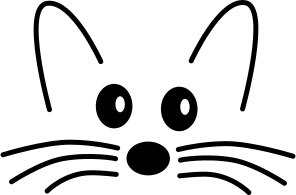
\includegraphics[width=1.4em]{squeak-logo}}}
\newcommand{\dothis}[1]{%
	\medskip
	\noindent\dothisicon
	\ifx#1\empty\else\quad\emph{#1}\fi
	\par\smallskip\nopagebreak}
% NB: To use this in an individual chapter, you must set:
%\graphicspath{{figures/} {../figures/}}
% at the head of the chapter.  Don't forget the final /
%=============================================================
%:Reader hints (hint)
%
% Indicates a non-obvious consequence 
\newcommand{\hint}[1]{\vspace{1ex}\noindent\fbox{\textsc{Astuce}} \emph{#1}}
%=================================================================
% graphics for Morphic handles
\newcommand{\grabHandle}{\raisebox{-0.2ex}{
\includegraphics[width=1em]{blackHandle}}}
\newcommand{\moveHandle}{\raisebox{-0.2ex}{
\includegraphics[width=1em]{moveHandle}}}
\newcommand{\debugHandle}{\raisebox{-0.2ex}{
\includegraphics[width=1em]{debugHandle}}}
% squeak-fr (added for Morphic handles)
\newcommand{\rotateHandle}{\raisebox{-0.2ex}{
\includegraphics[width=1em]{rotateHandle}}}
\newcommand{\viewerHandle}{\raisebox{-0.2ex}{
\includegraphics[width=1em]{viewerHandle}}}
% squeak-fr (add cloverHandle to use \clover in QuickTour.tex as alias
% todo 

%=============================================================
%:Highlighting Important stuff (doublebox)
%
% From Seaside book ...
\newsavebox{\SavedText}
\newlength{\InnerBoxRule}\setlength{\InnerBoxRule}{.75\fboxrule}
\newlength{\OuterBoxRule}\setlength{\OuterBoxRule}{1.5\fboxrule}
\newlength{\BoxSeparation}\setlength{\BoxSeparation}{1.5\fboxrule}
\addtolength{\BoxSeparation}{.5pt}
\newlength{\SaveBoxSep}\setlength{\SaveBoxSep}{2\fboxsep}
%
\newenvironment{doublebox}{\begin{lrbox}{\SavedText}
    \begin{minipage}{.75\textwidth}}
    {\end{minipage}\end{lrbox}\begin{center}
    \setlength{\fboxsep}{\BoxSeparation}\setlength{\fboxrule}{\OuterBoxRule}
    \fbox{\setlength{\fboxsep}{\SaveBoxSep}\setlength{\fboxrule}{\InnerBoxRule}%
      \fbox{\usebox{\SavedText}}}
  \end{center}}
% Use this:
%\newcommand{\important}[1]{\begin{doublebox}#1\end{doublebox}}


\newcommand{\important}[1]{
\noindent\rule{\textwidth}{2pt}\par
\textbf{Important!} #1 \par
\noindent\rule{\textwidth}{2pt}}

\newcommand{\note}[1]{
\noindent\rule{\textwidth}{2pt}\par
\noindent\textbf{Note} #1\par
\noindent\rule{\textwidth}{2pt}}

%=============================================================
%:Section depth
\setcounter{secnumdepth}{2}
%% for this to happen start the file with
%\ifx\wholebook\relax\else
%\input{../common.tex}
%\begin{document}
%\fi
% and terminate by
% \ifx\wholebook\relax\else\end{document}\fi

\DeclareGraphicsExtensions{.pdf, .jpg, .png}
%=============================================================
%:PDF setup
\hypersetup{
%   a4paper,
%   pdfstartview=FitV,
%   colorlinks,
%   linkcolor=darkblue,
%   citecolor=darkblue,
%   pdftitle={Squeak by Example},
pdftitle={Squeak par l'exemple},
   pdfauthor={Andrew Black, St\'ephane Ducasse,	Oscar Nierstrasz,
Damien Pollet},
   pdfkeywords={Smalltalk, Squeak, Programmation Orient\'ee Objet},
pdfsubject={Informatique, Computer Science}
}
%=============================================================
%:Page layout and appearance
%
% \renewcommand{\headrulewidth}{0pt}
\renewcommand{\chaptermark}[1]{\markboth{#1}{}}
\renewcommand{\sectionmark}[1]{\markright{\thesection\ #1}}
\renewpagestyle{plain}[\small\itshape]{%
	\setheadrule{0pt}%
	\sethead[][][]{}{}{}%
	\setfoot[][][]{}{}{}}
\renewpagestyle{headings}[\small\itshape]{%
	\setheadrule{0pt}%
	\setmarks{chapter}{section}%
	\sethead[\thepage][][\chaptertitle]{\sectiontitle}{}{\thepage}%
	\setfoot[][][]{}{}{}}
% pagestyle for tableofcontents + index (martial: 2008/04/23)
\newpagestyle{newheadings}[\small\itshape]{%
	\setheadrule{0pt}%
	\setmarks{chapter}{section}%
	\sethead[\thepage][][\chaptertitle]{\chaptertitle}{}{\thepage}%
	\setfoot[][][]{}{}{}}
%=============================================================
%:Title section setup and TOC numbering depth
\setcounter{secnumdepth}{1}
\setcounter{tocdepth}{1}
\titleformat{\part}[display]{\centering}{\huge\partname\ \thepart}{1em}{\Huge\textbf}[]
\titleformat{\chapter}[display]{}{\huge\chaptertitlename\ \thechapter}{1em}{\Huge\raggedright\textbf}[]
\titlecontents{part}[3pc]{%
		\pagebreak[2]\addvspace{1em plus.4em minus.2em}%
		\leavevmode\large\bfseries}
	{\contentslabel{3pc}}{\hspace*{-3pc}}
	{}[\nopagebreak]
\titlecontents{chapter}[3pc]{%
		\pagebreak[0]\addvspace{1em plus.2em minus.2em}%
		\leavevmode\bfseries}
	{\contentslabel{3pc}}{}
	{\hfill\contentspage}[\nopagebreak]
\dottedcontents{section}[3pc]{}{3pc}{1pc}
\dottedcontents{subsection}[3pc]{}{0pc}{1pc}
% \dottedcontents{subsection}[4.5em]{}{0pt}{1pc}
% Make \cleardoublepage insert really blank pages http://www.tex.ac.uk/cgi-bin/texfaq2html?label=reallyblank
\let\origdoublepage\cleardoublepage
\newcommand{\clearemptydoublepage}{%
  \clearpage
  {\pagestyle{empty}\origdoublepage}}
\let\cleardoublepage\clearemptydoublepage % see http://www.tex.ac.uk/cgi-bin/texfaq2html?label=patch
%=============================================================
%:FAQ macros (for FAQ chapter)
\newtheorem{faq}{FAQ}
\newcommand{\answer}{\paragraph{R\'eponse}\ }
%=============================================================
%:Listings package configuration
\usepackage{listings}
\newcommand{\caret}{\makebox{\raisebox{0.4ex}{\footnotesize{$\wedge$}}}}
\lstdefinelanguage{Smalltalk}{
%  morekeywords={self,super,true,false,nil,thisContext}, % This is overkill
  morestring=[d]',
  morecomment=[s]{"}{"},
  alsoletter={\#:},
  escapechar={!},
  escapebegin=\itshape, % comment-like by default (Martial 11/2007)
  literate=
    {BANG}{!}1
    {UNDERSCORE}{\_}1
    {\\st}{Smalltalk}9 % convenience -- in case \st occurs in code
    % {'}{{\textquotesingle}}1 % replaced by upquote=true in \lstset
    {_}{{$\leftarrow$}}1
    {>>>}{{\sep}}1
    {^}{{$\uparrow$}}1
    {~}{{$\sim$}}1
    {-}{{\sf -\hspace{-0.13em}-}}1  % the goal is to make - the same width as +
    {+}{\raisebox{0.08ex}{+}}1		% and to raise + off the baseline to match -
    {-->}{{\quad$\longrightarrow$\quad}}3
	, % Don't forget the comma at the end!
  tabsize=4
}[keywords,comments,strings]
% ajout pour les échappements dans les codes
% indispensable pour mettre le code en emphase (cf. Model.tex) 
\newcommand{\codeify}[1]{\NoAutoSpaceBeforeFDP#1\AutoSpaceBeforeFDP}
\newcommand{\normcomment}[1]{\emph{#1}} %cf. Streams
\newcommand{\normcode}[1]{\emph{\codeify{#1}}} %cf. Streams
\newcommand{\emcode}[1]{\textbf{\normcode{#1}}} % Martial 11/2007
\lstset{language=Smalltalk,
	basicstyle=\sffamily,
	keywordstyle=\color{black}\bfseries,
	% stringstyle=\ttfamily, % Ugly! do we really want this? -- on
	%commentstyle=\itshape,
	mathescape=true,
	showstringspaces=false,
	keepspaces=true,
	breaklines=true,
	breakautoindent=true,
	lineskip={-1pt}, % Ugly hack
	upquote=true, % straight quote; requires textcomp package
	columns=fullflexible} % no fixed width fonts
% In-line code (literal)
% Normally use this for all in-line code:
\newcommand{\ct}{\lstinline[mathescape=false,basicstyle={\sffamily\upshape}]}
% apb 2007.8.28 added the \upshape declaration to avoid getting italicized code in \dothis{ } sections.
% In-line code (latex enabled)
% Use this only in special situations where \ct does not work
% (within section headings ...):

% [squeak-fr] Modification de \lct suivant les indications de Martial Boniou
\newcommand{\lct}[1]{\textsf{\textup{\NoAutoSpaceBeforeFDP #1
\AutoSpaceBeforeFDP}}} %\xspace

% Use these for system categories and protocols:
\newcommand{\scat}[1]{\emph{\textsf{#1}}\xspace}
\newcommand{\pkg}[1]{\emph{\textsf{#1}}\xspace}
\newcommand{\prot}[1]{\emph{\textsf{#1}}\xspace}
% Code environments
% NB: the arg is for tests
% Only code and example environments may be tests
\lstnewenvironment{code}[1]{%
	\lstset{%
		frame=lines,
		mathescape=false
	}
}{}
\def\ignoredollar#1{}
%=============================================================
%:Code environments (method, script ...)
% NB: the third arg is for tests
% Only code and example environments may be tests
\lstnewenvironment{example}[3][defaultlabel]{%
	\renewcommand{\lstlistingname}{Exemple}%
	\lstset{
		frame=lines,
		mathescape=false,
		caption={\emph{#2}},
		label={eg:#1}
	}
}{}
\lstnewenvironment{script}[2][defaultlabel]{%
\renewcommand{\lstlistingname}{Script}%
	\lstset{
		frame=lines,
		mathescape=false,
		name={Script},
		caption={\emph{#2}},
		label={scr:#1}
	}
}{}
%I could not find a way yo get the Experiment #numb followed by the caption in a black box
%\colorbox{black}{\makebox[\textwidth]{  \color{white} {\large {\bfseries Experiment 3-1 (crear i moure un robot)}} }}
\lstnewenvironment{experiment}[2][defaultlabel]{%
%\noindent\rule{\textwidth}{2pt}\vspace{-0.8cm}
\renewcommand{\lstlistingname}{Experiment}%
	\lstset{
		frame=none,
		rulecolor=\color{black},
		mathescape=false,
		name={Experiment},
		caption={\emph{#2}},
		label={scr:#1}
	}
}{%\vspace{-0.5cm}\noindent\rule{\textwidth}{2pt}
}

\lstnewenvironment{method}[2][defaultlabel]{%
	\renewcommand{\lstlistingname}{Method}%
	\lstset{
		frame=lines,
		mathescape=false,
		name={M\'ethode},
		caption={\emph{#2}},
		label={mth:#1}
	}
}{}
\lstnewenvironment{methods}[2][defaultlabel]{% just for multiple methods at once
	\renewcommand{\lstlistingname}{Methods}%
	\lstset{
		frame=lines,
		mathescape=false,
		name={M\'ethode},
		caption={\emph{#2}},
		label={mth:#1}
	}
}{}
\lstnewenvironment{numMethod}[2][defaultlabel]{%
	\renewcommand{\lstlistingname}{Method}%
	\lstset{
		numbers=left,
		numberstyle={\tiny\sffamily},
		frame=lines,
		mathescape=false,
		name={M\'ethode},
		caption={\emph{#2}},
		label={mth:#1}
	}
}{}
% \lstnewenvironment{classdef}[2][defaultlabel]{%
% 	\renewcommand{\lstlistingname}{Classe}%
% 	\lstset{
% 		frame=lines,
% 		mathescape=false,
% 		name={Classe},
% 		caption={\emph{#2}},
% 		label={cls:#1}
% 	}
% }{}

%%%%%%%%%%%%%%%%%%%%%%%%%%%%%%%%%%%%%%%%%%%%%%%%%%%%%%%%%%%%%%%%%%%%%%%%%%%%%%%%%%%%%%%%%%%%%%%%%
%%From the original book latex template
%%%%%%%%%%%%%%%%%%%%%%%%%%%%%%%%%%%%%%%%%%%%%%%%%%%%%%%%%%%%%%%%%%%%%%%%%%%%%%%%%%%%%%%%%%%%%%%%%
\theoremstyle{break}
{\theorembodyfont{\rmfamily}\theoremstyle{break}
\newtheorem{privScript}{Script}[chapter]
%\newtheorem{privMethod}{Method}[chapter]
\newtheorem{privExercise}{Experiment}[chapter]}

% \theoremstyle{break}
% {\theorembodyfont{\rmfamily} \newtheorem{privMethod}{Method}[chapter]}

%class
\theoremstyle{break}
{\theorembodyfont{\rmfamily} \newtheorem{privClassDef}{Class}[chapter]}

%important
\theoremstyle{break}
{\theorembodyfont{\rmfamily} \newtheorem{privTemplate}{Important Messages}[chapter]}

% experiment
\newenvironment{exercise}
    {\begin{privExercise}\mbox{}\\}
    {\end{privExercise}}


%%% for figure
\newsavebox{\ScriptFigure}
\newlength{\ScriptWidth}
\newlength{\FigureWidth}

%%%%%%%%%%%%%%%%%%%%%%%%%%%%%%%%%%%%%%%%%%%%%%%%%%%%%%%%%%%%%%%%%%%%%%%%%%%%%%%%
\newenvironment{scriptfig}[3][0.6]
   {\setlength{\ScriptWidth}{\linewidth*\real{#1}}%
   \setlength{\FigureWidth}{\linewidth-(\linewidth*\real{#1})}%
   \savebox{\ScriptFigure}%
	{\parbox{\FigureWidth}{\includegraphics[width=0.98\FigureWidth]{#2}}}%
   \par\noindent\begin{minipage}{\linewidth}\hrule\vskip 0.2cm\begin{minipage}[c]{\ScriptWidth}%
   \begin{stefscript}[{\em #3}]\begin{alltt}\sffamily}
   {\end{alltt}\end{stefscript}\end{minipage}\hfill
   \usebox{\ScriptFigure}
   \vskip 1ex\hrule\end{minipage}\vskip 1ex\par}

%%%%%%%%%%%%%%%%%%%%%%%%%%%%%%%%%%%%%%%%%%%%%%%%%%%%%%%%%%%%%%%%%%%%%%%%%%%%%%%%
%% to be able to specify the complete set of values for includegraphics
%% may be will be changed but not the interface
\newenvironment{scriptfigwithsize}[3][0.6]
   {\setlength{\ScriptWidth}{\linewidth*\real{#1}}%
   \setlength{\FigureWidth}{\linewidth-(\linewidth*\real{#1})}%
   \savebox{\ScriptFigure}{\parbox{\FigureWidth}{\raggedleft{#2}}}%
   \par\noindent\begin{minipage}{\linewidth}\hrule\vskip 0.3cm\begin{minipage}[c]{\ScriptWidth}%
   \begin{stefscript}[{\em #3}]\begin{alltt}\sffamily}
   {\end{alltt}\end{stefscript}\end{minipage}\hfill
   \usebox{\ScriptFigure}
   \vskip 1ex\hrule\end{minipage}\vskip 1ex\par}

% \newenvironment{methodfig}[2][0.6]
%    {\setlength{\ScriptWidth}{\linewidth*\real{#1}}%
%    \setlength{\FigureWidth}{\linewidth-(\linewidth*\real{#1})}%
%    \savebox{\ScriptFigure}{\parbox{\FigureWidth}{\includegraphics[width=.98\FigureWidth]{#2}}}%
%    \par\noindent\rule{\linewidth}{1mm}
%    \\[-0.3cm]\noindent\rule{\linewidth}{0.1mm}
%    \noindent\begin{minipage}[c]{\ScriptWidth}\begin{privMethod}\begin{alltt}\sffamily}
%    {\end{alltt}\end{privMethod}\end{minipage}\hfill
%    \usebox{\ScriptFigure} \vskip 1ex\hrule\vskip 1ex\par}

% \newenvironment{method}
% {\par\noindent\begin{minipage}{\linewidth}\vspace{0.2cm}\begin{privMethod}\begin{nminipage}\vspace{-0.2cm}\rule{\linewidth}{1mm}\\[-0.6cm]\rule{\linewidth}{0.1mm}\end{nminipage}\hspace*{\scriptindent}\codesize\begin{nalltt}\vspace{-0.2cm}}
% {\end{nalltt}\normalsize\vspace{-0.1cm}\hrule\end{privMethod}\vspace{0.2cm}\end{minipage}}


% \newenvironment{classdef}
% {\par\noindent\begin{minipage}{\linewidth}\vspace{0.2cm}\begin{privClassDef}\begin{nminipage}\vspace{-0.2cm}\rule{\linewidth}{1mm}\\[-0.6cm]\rule{\linewidth}{0.1mm}\end{nminipage}\hspace*{\scriptindent}\codesize\begin{nalltt}\vspace{-0.2cm}}
% {\end{nalltt}\normalsize\vspace{-0.1cm}\hrule\end{privClassDef}\vspace{0.2cm}\end{minipage}}


% \newenvironment{template}
% {\par\noindent\begin{minipage}{\linewidth}\vspace{0.3cm}\begin{privTemplate}\begin{nminipage}\vspace{-0.4cm}\rule{\linewidth}{0.1mm}\end{nminipage}\hspace*{\scriptindent}\begin{nalltt}\vspace{-0.7cm}}
% {\end{nalltt}\vspace{-0.1cm}\hrule\end{privTemplate}\end{minipage}\vspace{0.3cm}}

\newenvironment{exofig}[2][0.7]
   {\setlength{\ScriptWidth}{\linewidth*\real{#1}}
   \setlength{\FigureWidth}{\linewidth-(\linewidth*\real{#1})}
   \savebox{\ScriptFigure}{\parbox{\FigureWidth}{\raggedleft{\includegraphics[width=.98\FigureWidth]{#2}}}}
   \par\noindent\begin{minipage}{\linewidth}\hrule\vskip 0.3cm\begin{minipage}[c]{\ScriptWidth}%
   \begin{privExercise}}
   {\end{privExercise}\end{minipage}\hfill
   \usebox{\ScriptFigure}
   \vskip 1ex\hrule\end{minipage}\vskip 1ex\par}

\newenvironment{exofigwithsize}[2][0.7]
   {\setlength{\ScriptWidth}{\linewidth*\real{#1}}
   \setlength{\FigureWidth}{\linewidth-(\linewidth*\real{#1})}
   \savebox{\ScriptFigure}{\parbox{\FigureWidth}{\raggedleft{#2}}}
   \par\noindent\begin{minipage}{\linewidth}\hrule\vskip 0.3cm\begin{minipage}[c]{\ScriptWidth}%
   \begin{privExercise}}
   {\end{privExercise}\end{minipage}\hfill\usebox{\ScriptFigure}
   \vskip 1ex\hrule\end{minipage}\vskip 1ex\par}

\newenvironment{exofigwithsizeandtitle}[3][0.7]
   {\setlength{\ScriptWidth}{\linewidth*\real{#1}}
   \setlength{\FigureWidth}{\linewidth-(\linewidth*\real{#1})}
   \savebox{\ScriptFigure}{\parbox{\FigureWidth}{\raggedleft{#2}}}
   \vskip 0.3cm\par\noindent\begin{minipage}{\linewidth}\hrule\vskip 0.1cm\begin{minipage}[c]{\ScriptWidth}%
   \begin{privExercise}[\em{#3}]}
   {\end{privExercise}\end{minipage}\hfill\usebox{\ScriptFigure}
   \vskip 1ex\hrule\end{minipage}\vskip 1ex\par}

\newenvironment{exofigwithtitle}[3][0.7]
   {\setlength{\ScriptWidth}{\linewidth*\real{#1}}
   \setlength{\FigureWidth}{\linewidth-(\linewidth*\real{#1})}
   \savebox{\ScriptFigure}{\parbox{\FigureWidth}{\raggedleft{\includegraphics[width=.98\FigureWidth]{#2}}}}
   \par\noindent\begin{minipage}{\linewidth}\hrule\vskip 0.3cm\begin{minipage}[c]{\ScriptWidth}%
   \begin{privExercise}[\em{#3}]}
   {\end{privExercise}\end{minipage}\hfill
   \usebox{\ScriptFigure}
   \vskip 1ex\hrule\end{minipage}\vskip 1ex\par}


\newenvironment{exonofigwithtitle}[3][0.7]
   {\setlength{\ScriptWidth}{\linewidth*\real{#1}}
   \setlength{\FigureWidth}{\linewidth-(\linewidth*\real{#1})}
   \savebox{\ScriptFigure}{\parbox{\FigureWidth}{\raggedleft{\includegraphics[width=.98\FigureWidth]{#2}}}}
   \par\noindent\begin{minipage}{\linewidth}\hrule\vskip 0.3cm\begin{minipage}[c]{\ScriptWidth}%
   \begin{privExercise}[\em{#3}]}
   {\end{privExercise}\end{minipage}\hfill
   \usebox{\ScriptFigure}
   \vskip 1ex\hrule\end{minipage}\vskip 1ex\par}

\newenvironment{exonofig}
   {\par\noindent\begin{minipage}[t]{\linewidth}\noindent\begin{privExercise}}
   {\end{privExercise}\end{minipage}\vspace{0.5cm}\par}

\newenvironment{exonofigtitle}[1]
   {\par\noindent\begin{minipage}[t]{\linewidth}\noindent\begin{privExercise}[\em{#1}]}
   {\end{privExercise}\end{minipage}\vspace{0.5cm}\par}
		
% \newenvironment{solfig}[3][0.5]
%    {\setlength{\ScriptWidth}{\linewidth*\real{#1}}
%    \setlength{\FigureWidth}{\linewidth-\linewidth*\real{#1}}
%    \savebox{\ScriptFigure}{\parbox{\FigureWidth}{\includegraphics[width=.9\linewidth]{#2}}}
%    \par\noindent\vskip 1ex\hrule\vskip 1ex\begin{minipage}[t]{\ScriptWidth}
%    {\bf Solution #3} \begin{alltt}\sffamily}
%    {\end{alltt}\end{minipage}\hfill
%    \usebox{\ScriptFigure}
%    \vskip 1ex\hrule\vskip 1ex\par}
% 
% \newenvironment{solnofig}[1]
%    {\par\noindent\vskip 1ex\hrule\vskip 1ex\begin{minipage}[t]{\ScriptWidth}
%    {\bf Solution #1} \begin{alltt}\sffamily}
%    {\end{alltt}\end{minipage}\hfill
%    \vskip 1ex\hrule\vskip 1ex\par}
% 
% \newenvironment{exoscript}[3][0.5]
%    {\setlength{\ScriptWidth}{\linewidth*\real{#1}}
%     \setlength{\FigureWidth}{\linewidth-\linewidth*\real{#1}}
%     \savebox{\ScriptFigure}{\begin{minipage}\begin{alltt}\sffamily#3\end{alltt}\end{minipage}}
%     \par\noindent\vskip 1ex\hrule\vskip 1ex\begin{minipage}[t]{\ScriptWidth}
%     \begin{privExercise}}
%     {\end{privExercise}\end{minipage}\hfill
%     \usebox{\ScriptFigure}
% \vskip 1ex\hrule\vskip 1ex\par}


%%%%%%%%%%%%%%%%%%%%%%%%%%%%%%%%%%%%%%%%%%%%%%%%%%%%%%%%%%%%%%%%
%% Define the indentation from which the code script starts
%\newlength{\scriptindent}
%\setlength{\scriptindent}{.3cm}
%%%%%%%%%%%%%%%%%%%%%%%%%%%%%%%%%%%%%%%%%%%%%%%%%%%%%%%%%%%%%%%%
%% Method presentation 
%\newlength{\methodindent}
%\newlength{\methodwordlength}
%\newlength{\aftermethod}
%\setlength{\methodindent}{0.2cm}
%\settowidth{\methodwordlength}{\ M\'ethode\ }

%%%%%%%%%%%%%%%%%%%%%%%%%%%%%%%%%%%%%%%%%%%%%%%%%%%%%%%%%%%%%%%%
\theoremstyle{break}
{\theorembodyfont{\rmfamily} \newtheorem{fonction}{Script}[chapter]}

\newsavebox{\fminibox}
\newlength{\fminilength}
% Fait un truc encadre
\newenvironment{fminipage}[1][\linewidth]
  {\setlength{\fminilength}{#1-2\fboxsep-2\fboxrule}
        \begin{lrbox}{\fminibox}\begin{minipage}{\fminilength}}
  { \end{minipage}\end{lrbox}\noindent\fbox{\usebox{\fminibox}}}

% Pareil mais pas encadre (a utiliser pour ne pas couper une fonction en 2)
\newenvironment{nminipage}[1][\linewidth]
  {\setlength{\fminilength}{#1}
        \begin{lrbox}{\fminibox}\begin{minipage}{\fminilength}}
  { \end{minipage}\end{lrbox}\noindent\mbox{\usebox{\fminibox}}}

% Un alltt encadre
\newenvironment{falltt}
  {\vspace*{0.3cm}\begin{fminipage}\begin{alltt}\ttfamily}
  {\end{alltt}\end{fminipage}\vspace*{0.3cm}}

% Un alltt pas encadre
\newenvironment{nalltt}
  {\vspace*{0.3cm}\begin{nminipage}\begin{alltt}\sffamily}
  {\end{alltt}\end{nminipage}\vspace*{0.3cm}}

% Une fonction encadree
\newenvironment{ffonction}[1]
  {\begin{fonction}[#1]\begin{fminipage}\begin{alltt}\ttfamily\rule{\linewidth}{0.5pt}}
{\end{alltt}\end{fminipage}\end{fonction}}


\theoremstyle{break}
{\theorembodyfont{\rmfamily} \newtheorem{stefscript}{Script}[chapter]}

\theoremstyle{break}
{\theorembodyfont{\rmfamily} \newtheorem{exampleScript}{Examples}[chapter]}


%%Not used
\newenvironment{ncscript}[1]
{\vspace{-0.5cm}\begin{stefscript}[#1]\begin{nalltt}\rule{\linewidth}{1.5pt}\vspace{-0.1cm}
\hspace*{\scriptindent}\begin{nalltt}}
{\end{nalltt}\vspace{-0.5cm}\hrule\end{nalltt}\end{stefscript}\vspace{-0.5cm}}
%%Not used
\newenvironment{soluscript}[1]
{\begin{nalltt}\textbf{Solution du script : #1.}\\
\rule{\linewidth}{1.5pt}
\hspace*{\scriptindent}\begin{nalltt}}
{\end{nalltt}\vspace{-0.5cm}\hrule\end{nalltt}\vspace{-0.5cm}\\}




\newenvironment{scriptwithtitle}[1]
{\vspace{-0.3cm}\begin{stefscript}[{\em #1}]\begin{nalltt}\rule{\linewidth}{1.5pt}\vspace{-0.3cm}\hspace*{\scriptindent}\begin{nalltt}\codesize}
{\normalsize\end{nalltt}\vspace{-0.2cm}\hrule\end{nalltt}\end{stefscript}\vspace{-0.5cm}}

\newenvironment{scriptwithouttitle}
{\vspace{-0.5cm}\begin{stefscript}\codesize\begin{nalltt}\rule{\linewidth}{1.5pt}\vspace{-0.1cm}
\hspace*{\scriptindent}\begin{nalltt}}
{\end{nalltt}\vspace{-0.5cm}\hrule\end{nalltt}\normalsize\end{stefscript}\vspace{-0.5cm}}

% \newenvironment{example}
% {\vspace{-0.5cm}\begin{exampleScript}\codesize\begin{nalltt}\rule{\linewidth}{1.5pt}\vspace{-0.1cm}\hspace*{\scriptindent}\begin{nalltt}}
% {\end{nalltt}\vspace{-0.2cm}\hrule\end{nalltt}\normalsize\end{exampleScript}\vspace{-0.5cm}}




























%=============================================================
%:Reserving space
% Usually need one more line than the actual lines of code
\newcommand{\needlines}[1]{\Needspace{#1\baselineskip}}
%=============================================================
%:Indexing macros
% Macros ending with "ind" generate text as well as an index entry
% Macros ending with "index" *only* generate an index entry
\newcommand{\ind}[1]{\index{#1}#1\xspace} % plain text
\newcommand{\subind}[2]{\index{#1!#2}#2\xspace} % show #2, subindex inder #1
\newcommand{\emphind}[1]{\index{#1}\emph{#1}\xspace} % emph #1
\newcommand{\emphsubind}[2]{\index{#1!#2}\emph{#2}\xspace} % show emph #2, subindex inder #1
\newcommand{\scatind}[1]{\index{#1@\textsf{#1} (cat\'egorie)}\scat{#1}} % category
\newcommand{\protind}[1]{\index{#1@\textsf{#1} (protocole)}\prot{#1}} % protocol
% \newcommand{\clsind}[1]{\index{#1@\textsf{#1} (class)}\ct{#1}\xspace}
\newcommand{\clsind}[1]{\index{#1!\#@(classe)}\ct{#1}\xspace} % class
\newcommand{\cvind}[1]{\index{#1@\textsf{#1} (variable de classe)}\ct{#1}\xspace} % class var
\newcommand{\glbind}[1]{\index{#1@\textsf{#1} (globale)}\ct{#1}\xspace} % global
\newcommand{\patind}[1]{\index{#1@#1 (patron)}\ct{#1}\xspace} % pattern
\newcommand{\pvind}[1]{\index{#1@\textsf{#1} (pseudo-variable)}\ct{#1}\xspace} % pseudo variable
% [squeak - fr]Martial: I found the following cleaner (should be
% merged in SBE for self and super)
\newcommand{\subpvindex}[2]{\index{#1@\textsf{#1} (pseudo-variable)!#2}}
\newcommand{\subpvind}[2]{\index{#1@\textsf{#1} (pseudo-variable)!#2}#2\xspace}
% used in Model.tex
\newcommand{\mthind}[2]{\index{#1!#2@\ct{#2}}\ct{#2}\xspace} % show method name only
\newcommand{\lmthind}[2]{\index{#1!#2@\ct{#2}}\lct{#2}\xspace} % show method name only
\newcommand{\cmind}[2]{\index{#1!#2@\ct{#2}}\ct{#1>>>#2}\xspace} % show class>>method
\newcommand{\toolsflapind}{\index{onglet Tools}\toolsflap} % index tools flap
% The following only generate an index entry:
% \newcommand{\clsindex}[1]{\index{#1@\textsf{#1} (class)}}
\newcommand{\clsindex}[1]{\index{#1!\#@(classe)}} % class
\newcommand{\cmindex}[2]{\index{#1!#2@\ct{#2}}} % class>>method
\newcommand{\cvindex}[1]{\index{#1@\textsf{#1} (variable de classe)}} % class var
\newcommand{\glbindex}[1]{\index{#1@\textsf{#1} (globale)}}% global
\newcommand{\pvindex}[1]{\index{#1@\textsf{#1} (pseudo-variable)}}% pseudo var
\newcommand{\seeindex}[2]{\index{#1|see{#2}}} % #1, see #2
\newcommand{\scatindex}[1]{\index{#1@\textsf{#1} (cat\'egorie)}} % category
\newcommand{\protindex}[1]{\index{#1@\textsf{#1} (protocole)}} % protocol
% How can we have the main entry page numbers in bold yet not break the hyperlink?
\newcommand{\boldidx}[1]{{\bf #1}} % breaks hyperlink
%\newcommand{\indmain}[1]{\index{#1|boldidx}#1\xspace} % plain text, main entry
%\newcommand{\emphsubindmain}[2]{\index{#1!#2|boldidx}\emph{#2}\xspace} % subindex, main entry
%\newcommand{\subindmain}[2]{\index{#1!#2|boldidx}#2\xspace} % subindex, main entry
%\newcommand{\clsindmain}[1]{\index{#1@\textsf{#1} (class)|boldidx}\ct{#1}\xspace}
%\newcommand{\clsindmain}[1]{\index{#1!\#@(class)|boldidx}\ct{#1}\xspace} % class main
%\newcommand{\indexmain}[1]{\index{#1|boldidx}} % main index entry only
\newcommand{\indmain}[1]{\index{#1}#1\xspace} 
\newcommand{\emphsubindmain}[2]{\index{#1!#2}\emph{#2}\xspace} % subindex, main entry
\newcommand{\subindmain}[2]{\index{#1!#2}#2\xspace} % subindex, main entry
%\newcommand{\clsindmain}[1]{\index{#1@\textsf{#1} (class)}\ct{#1}\xspace}
\newcommand{\clsindmain}[1]{\index{#1!\#@(classe)}\ct{#1}\xspace} % class main
\newcommand{\indexmain}[1]{\index{#1}} 
%=============================================================
%:Code macros
% some constants
\newcommand{\codesize}{\small}
\newcommand{\codefont}{\sffamily}
\newcommand{\cat}[1]{\textit{Dans la cat\'egorie #1}}%%To remove later
\newlength{\scriptindent}
\setlength{\scriptindent}{.3cm}
%% Method presentation constants
\newlength{\methodindent}
\newlength{\methodwordlength}
\newlength{\aftermethod}
\setlength{\methodindent}{0.2cm}
\settowidth{\methodwordlength}{\ M\'ethode\ }
%=============================================================
%:Smalltalk macros
%\newcommand{\sep}{{$\gg$}}
\newcommand{\sep}{\mbox{>>}}
\newcommand{\self}{\ct{self}\xspace}
\newcommand{\super}{\ct{super}\xspace}
\newcommand{\nil}{\ct{nil}\xspace}
%=============================================================
% be less conservative about float placement
% these commands are from http://www.tex.ac.uk/cgi-bin/texfaq2html?label=floats
\renewcommand{\topfraction}{.9}
\renewcommand{\bottomfraction}{.9}
\renewcommand{\textfraction}{.1}
\renewcommand{\floatpagefraction}{.85}
\renewcommand{\dbltopfraction}{.66}
\renewcommand{\dblfloatpagefraction}{.85}
\setcounter{topnumber}{9}
\setcounter{bottomnumber}{9}
\setcounter{totalnumber}{20}
\setcounter{dbltopnumber}{9}
%=============================================================
%% [Squeak-fr]
% pour identifier les zones de texte à corriger d'urgence!
\newcommand{\arevoir}[1]{#1}
% \traduit utilisé dans Model.tex
\newcommand{\traduit}[1]{\footnote[2]{#1}}
% changeset alias
\newcommand{\changeset}{\emph{change set}\xspace}
\newcommand{\changesets}{\emph{change sets}\xspace}
% callback alias
\newcommand{\callback}{\emph{callback}\xspace}
% blobmorph alias (QuickTour->blob)
\newcommand{\blobmorph}{\emph{blob}\xspace}
% repository
\newcommand{\squeaksource}{\textsf{SqueakSource}\xspace}
\newcommand{\sourceforge}{\textsf{SourceForge}\xspace}
% L'onglet Tools
\newcommand{\Toolsflap}{L'onglet \textit{Tools}\xspace}
% Mac OS X
\newcommand{\macosx}{\mbox{Mac OS X}\xspace}
% code en francais (uniquement dans le chapitre BasicClasses)
\newcommand{\codefrench}[1]{\NoAutoSpaceBeforeFDP\texttt{#1}\AutoSpaceBeforeFDP\xspace}
% mantra du modele objet (suite a l'erreur de martial)
\newcommand{\Mantra}{Tout est objet\xspace}
\newcommand{\mantra}{\MakeLowercase{\Mantra}\xspace}
% césure
\hyphenation{Omni-Brow-ser}
\hyphenation{m\'e-tho-de} % erreur de cesure commune
\hyphenation{m\'e-tho-des}
\hyphenation{e-xem-ple}
\hyphenation{en-re-gi-stre}
\hyphenation{a-na-ly-seur}
\hyphenation{glo-ba-le}
\hyphenation{fi-gu-re}
\hyphenation{vi-si-bles}
\hyphenation{cor-res-pon-dan-te}
\hyphenation{Work-space}
%=============================================================
% apb doesn't like paragraphs to run in to each other without a break
\parskip 1ex
%=============================================================
%:Stuff to check, merge or deprecate
%\setlength{\marginparsep}{2mm}
%\renewcommand{\baselinestretch}{1.1}
%=============================================================

%\begin{document}
%\fi
% and terminate by
% \ifx\wholebook\relax\else\end{document}\fi

\DeclareGraphicsExtensions{.pdf, .jpg, .png}
%=============================================================
%:PDF setup
\hypersetup{
%   a4paper,
%   pdfstartview=FitV,
%   colorlinks,
%   linkcolor=darkblue,
%   citecolor=darkblue,
%   pdftitle={Squeak by Example},
pdftitle={Squeak par l'exemple},
   pdfauthor={Andrew Black, St\'ephane Ducasse,	Oscar Nierstrasz,
Damien Pollet},
   pdfkeywords={Smalltalk, Squeak, Programmation Orient\'ee Objet},
pdfsubject={Informatique, Computer Science}
}
%=============================================================
%:Page layout and appearance
%
% \renewcommand{\headrulewidth}{0pt}
\renewcommand{\chaptermark}[1]{\markboth{#1}{}}
\renewcommand{\sectionmark}[1]{\markright{\thesection\ #1}}
\renewpagestyle{plain}[\small\itshape]{%
	\setheadrule{0pt}%
	\sethead[][][]{}{}{}%
	\setfoot[][][]{}{}{}}
\renewpagestyle{headings}[\small\itshape]{%
	\setheadrule{0pt}%
	\setmarks{chapter}{section}%
	\sethead[\thepage][][\chaptertitle]{\sectiontitle}{}{\thepage}%
	\setfoot[][][]{}{}{}}
% pagestyle for tableofcontents + index (martial: 2008/04/23)
\newpagestyle{newheadings}[\small\itshape]{%
	\setheadrule{0pt}%
	\setmarks{chapter}{section}%
	\sethead[\thepage][][\chaptertitle]{\chaptertitle}{}{\thepage}%
	\setfoot[][][]{}{}{}}
%=============================================================
%:Title section setup and TOC numbering depth
\setcounter{secnumdepth}{1}
\setcounter{tocdepth}{1}
\titleformat{\part}[display]{\centering}{\huge\partname\ \thepart}{1em}{\Huge\textbf}[]
\titleformat{\chapter}[display]{}{\huge\chaptertitlename\ \thechapter}{1em}{\Huge\raggedright\textbf}[]
\titlecontents{part}[3pc]{%
		\pagebreak[2]\addvspace{1em plus.4em minus.2em}%
		\leavevmode\large\bfseries}
	{\contentslabel{3pc}}{\hspace*{-3pc}}
	{}[\nopagebreak]
\titlecontents{chapter}[3pc]{%
		\pagebreak[0]\addvspace{1em plus.2em minus.2em}%
		\leavevmode\bfseries}
	{\contentslabel{3pc}}{}
	{\hfill\contentspage}[\nopagebreak]
\dottedcontents{section}[3pc]{}{3pc}{1pc}
\dottedcontents{subsection}[3pc]{}{0pc}{1pc}
% \dottedcontents{subsection}[4.5em]{}{0pt}{1pc}
% Make \cleardoublepage insert really blank pages http://www.tex.ac.uk/cgi-bin/texfaq2html?label=reallyblank
\let\origdoublepage\cleardoublepage
\newcommand{\clearemptydoublepage}{%
  \clearpage
  {\pagestyle{empty}\origdoublepage}}
\let\cleardoublepage\clearemptydoublepage % see http://www.tex.ac.uk/cgi-bin/texfaq2html?label=patch
%=============================================================
%:FAQ macros (for FAQ chapter)
\newtheorem{faq}{FAQ}
\newcommand{\answer}{\paragraph{R\'eponse}\ }
%=============================================================
%:Listings package configuration
\usepackage{listings}
\newcommand{\caret}{\makebox{\raisebox{0.4ex}{\footnotesize{$\wedge$}}}}
\lstdefinelanguage{Smalltalk}{
%  morekeywords={self,super,true,false,nil,thisContext}, % This is overkill
  morestring=[d]',
  morecomment=[s]{"}{"},
  alsoletter={\#:},
  escapechar={!},
  escapebegin=\itshape, % comment-like by default (Martial 11/2007)
  literate=
    {BANG}{!}1
    {UNDERSCORE}{\_}1
    {\\st}{Smalltalk}9 % convenience -- in case \st occurs in code
    % {'}{{\textquotesingle}}1 % replaced by upquote=true in \lstset
    {_}{{$\leftarrow$}}1
    {>>>}{{\sep}}1
    {^}{{$\uparrow$}}1
    {~}{{$\sim$}}1
    {-}{{\sf -\hspace{-0.13em}-}}1  % the goal is to make - the same width as +
    {+}{\raisebox{0.08ex}{+}}1		% and to raise + off the baseline to match -
    {-->}{{\quad$\longrightarrow$\quad}}3
	, % Don't forget the comma at the end!
  tabsize=4
}[keywords,comments,strings]
% ajout pour les échappements dans les codes
% indispensable pour mettre le code en emphase (cf. Model.tex) 
\newcommand{\codeify}[1]{\NoAutoSpaceBeforeFDP#1\AutoSpaceBeforeFDP}
\newcommand{\normcomment}[1]{\emph{#1}} %cf. Streams
\newcommand{\normcode}[1]{\emph{\codeify{#1}}} %cf. Streams
\newcommand{\emcode}[1]{\textbf{\normcode{#1}}} % Martial 11/2007
\lstset{language=Smalltalk,
	basicstyle=\sffamily,
	keywordstyle=\color{black}\bfseries,
	% stringstyle=\ttfamily, % Ugly! do we really want this? -- on
	%commentstyle=\itshape,
	mathescape=true,
	showstringspaces=false,
	keepspaces=true,
	breaklines=true,
	breakautoindent=true,
	lineskip={-1pt}, % Ugly hack
	upquote=true, % straight quote; requires textcomp package
	columns=fullflexible} % no fixed width fonts
% In-line code (literal)
% Normally use this for all in-line code:
\newcommand{\ct}{\lstinline[mathescape=false,basicstyle={\sffamily\upshape}]}
% apb 2007.8.28 added the \upshape declaration to avoid getting italicized code in \dothis{ } sections.
% In-line code (latex enabled)
% Use this only in special situations where \ct does not work
% (within section headings ...):

% [squeak-fr] Modification de \lct suivant les indications de Martial Boniou
\newcommand{\lct}[1]{\textsf{\textup{\NoAutoSpaceBeforeFDP #1
\AutoSpaceBeforeFDP}}} %\xspace

% Use these for system categories and protocols:
\newcommand{\scat}[1]{\emph{\textsf{#1}}\xspace}
\newcommand{\pkg}[1]{\emph{\textsf{#1}}\xspace}
\newcommand{\prot}[1]{\emph{\textsf{#1}}\xspace}
% Code environments
% NB: the arg is for tests
% Only code and example environments may be tests
\lstnewenvironment{code}[1]{%
	\lstset{%
		frame=lines,
		mathescape=false
	}
}{}
\def\ignoredollar#1{}
%=============================================================
%:Code environments (method, script ...)
% NB: the third arg is for tests
% Only code and example environments may be tests
\lstnewenvironment{example}[3][defaultlabel]{%
	\renewcommand{\lstlistingname}{Exemple}%
	\lstset{
		frame=lines,
		mathescape=false,
		caption={\emph{#2}},
		label={eg:#1}
	}
}{}
\lstnewenvironment{script}[2][defaultlabel]{%
\renewcommand{\lstlistingname}{Script}%
	\lstset{
		frame=lines,
		mathescape=false,
		name={Script},
		caption={\emph{#2}},
		label={scr:#1}
	}
}{}
%I could not find a way yo get the Experiment #numb followed by the caption in a black box
%\colorbox{black}{\makebox[\textwidth]{  \color{white} {\large {\bfseries Experiment 3-1 (crear i moure un robot)}} }}
\lstnewenvironment{experiment}[2][defaultlabel]{%
%\noindent\rule{\textwidth}{2pt}\vspace{-0.8cm}
\renewcommand{\lstlistingname}{Experiment}%
	\lstset{
		frame=none,
		rulecolor=\color{black},
		mathescape=false,
		name={Experiment},
		caption={\emph{#2}},
		label={scr:#1}
	}
}{%\vspace{-0.5cm}\noindent\rule{\textwidth}{2pt}
}

\lstnewenvironment{method}[2][defaultlabel]{%
	\renewcommand{\lstlistingname}{Method}%
	\lstset{
		frame=lines,
		mathescape=false,
		name={M\'ethode},
		caption={\emph{#2}},
		label={mth:#1}
	}
}{}
\lstnewenvironment{methods}[2][defaultlabel]{% just for multiple methods at once
	\renewcommand{\lstlistingname}{Methods}%
	\lstset{
		frame=lines,
		mathescape=false,
		name={M\'ethode},
		caption={\emph{#2}},
		label={mth:#1}
	}
}{}
\lstnewenvironment{numMethod}[2][defaultlabel]{%
	\renewcommand{\lstlistingname}{Method}%
	\lstset{
		numbers=left,
		numberstyle={\tiny\sffamily},
		frame=lines,
		mathescape=false,
		name={M\'ethode},
		caption={\emph{#2}},
		label={mth:#1}
	}
}{}
% \lstnewenvironment{classdef}[2][defaultlabel]{%
% 	\renewcommand{\lstlistingname}{Classe}%
% 	\lstset{
% 		frame=lines,
% 		mathescape=false,
% 		name={Classe},
% 		caption={\emph{#2}},
% 		label={cls:#1}
% 	}
% }{}

%%%%%%%%%%%%%%%%%%%%%%%%%%%%%%%%%%%%%%%%%%%%%%%%%%%%%%%%%%%%%%%%%%%%%%%%%%%%%%%%%%%%%%%%%%%%%%%%%
%%From the original book latex template
%%%%%%%%%%%%%%%%%%%%%%%%%%%%%%%%%%%%%%%%%%%%%%%%%%%%%%%%%%%%%%%%%%%%%%%%%%%%%%%%%%%%%%%%%%%%%%%%%
\theoremstyle{break}
{\theorembodyfont{\rmfamily}\theoremstyle{break}
\newtheorem{privScript}{Script}[chapter]
%\newtheorem{privMethod}{Method}[chapter]
\newtheorem{privExercise}{Experiment}[chapter]}

% \theoremstyle{break}
% {\theorembodyfont{\rmfamily} \newtheorem{privMethod}{Method}[chapter]}

%class
\theoremstyle{break}
{\theorembodyfont{\rmfamily} \newtheorem{privClassDef}{Class}[chapter]}

%important
\theoremstyle{break}
{\theorembodyfont{\rmfamily} \newtheorem{privTemplate}{Important Messages}[chapter]}

% experiment
\newenvironment{exercise}
    {\begin{privExercise}\mbox{}\\}
    {\end{privExercise}}


%%% for figure
\newsavebox{\ScriptFigure}
\newlength{\ScriptWidth}
\newlength{\FigureWidth}

%%%%%%%%%%%%%%%%%%%%%%%%%%%%%%%%%%%%%%%%%%%%%%%%%%%%%%%%%%%%%%%%%%%%%%%%%%%%%%%%
\newenvironment{scriptfig}[3][0.6]
   {\setlength{\ScriptWidth}{\linewidth*\real{#1}}%
   \setlength{\FigureWidth}{\linewidth-(\linewidth*\real{#1})}%
   \savebox{\ScriptFigure}%
	{\parbox{\FigureWidth}{\includegraphics[width=0.98\FigureWidth]{#2}}}%
   \par\noindent\begin{minipage}{\linewidth}\hrule\vskip 0.2cm\begin{minipage}[c]{\ScriptWidth}%
   \begin{stefscript}[{\em #3}]\begin{alltt}\sffamily}
   {\end{alltt}\end{stefscript}\end{minipage}\hfill
   \usebox{\ScriptFigure}
   \vskip 1ex\hrule\end{minipage}\vskip 1ex\par}

%%%%%%%%%%%%%%%%%%%%%%%%%%%%%%%%%%%%%%%%%%%%%%%%%%%%%%%%%%%%%%%%%%%%%%%%%%%%%%%%
%% to be able to specify the complete set of values for includegraphics
%% may be will be changed but not the interface
\newenvironment{scriptfigwithsize}[3][0.6]
   {\setlength{\ScriptWidth}{\linewidth*\real{#1}}%
   \setlength{\FigureWidth}{\linewidth-(\linewidth*\real{#1})}%
   \savebox{\ScriptFigure}{\parbox{\FigureWidth}{\raggedleft{#2}}}%
   \par\noindent\begin{minipage}{\linewidth}\hrule\vskip 0.3cm\begin{minipage}[c]{\ScriptWidth}%
   \begin{stefscript}[{\em #3}]\begin{alltt}\sffamily}
   {\end{alltt}\end{stefscript}\end{minipage}\hfill
   \usebox{\ScriptFigure}
   \vskip 1ex\hrule\end{minipage}\vskip 1ex\par}

% \newenvironment{methodfig}[2][0.6]
%    {\setlength{\ScriptWidth}{\linewidth*\real{#1}}%
%    \setlength{\FigureWidth}{\linewidth-(\linewidth*\real{#1})}%
%    \savebox{\ScriptFigure}{\parbox{\FigureWidth}{\includegraphics[width=.98\FigureWidth]{#2}}}%
%    \par\noindent\rule{\linewidth}{1mm}
%    \\[-0.3cm]\noindent\rule{\linewidth}{0.1mm}
%    \noindent\begin{minipage}[c]{\ScriptWidth}\begin{privMethod}\begin{alltt}\sffamily}
%    {\end{alltt}\end{privMethod}\end{minipage}\hfill
%    \usebox{\ScriptFigure} \vskip 1ex\hrule\vskip 1ex\par}

% \newenvironment{method}
% {\par\noindent\begin{minipage}{\linewidth}\vspace{0.2cm}\begin{privMethod}\begin{nminipage}\vspace{-0.2cm}\rule{\linewidth}{1mm}\\[-0.6cm]\rule{\linewidth}{0.1mm}\end{nminipage}\hspace*{\scriptindent}\codesize\begin{nalltt}\vspace{-0.2cm}}
% {\end{nalltt}\normalsize\vspace{-0.1cm}\hrule\end{privMethod}\vspace{0.2cm}\end{minipage}}


% \newenvironment{classdef}
% {\par\noindent\begin{minipage}{\linewidth}\vspace{0.2cm}\begin{privClassDef}\begin{nminipage}\vspace{-0.2cm}\rule{\linewidth}{1mm}\\[-0.6cm]\rule{\linewidth}{0.1mm}\end{nminipage}\hspace*{\scriptindent}\codesize\begin{nalltt}\vspace{-0.2cm}}
% {\end{nalltt}\normalsize\vspace{-0.1cm}\hrule\end{privClassDef}\vspace{0.2cm}\end{minipage}}


% \newenvironment{template}
% {\par\noindent\begin{minipage}{\linewidth}\vspace{0.3cm}\begin{privTemplate}\begin{nminipage}\vspace{-0.4cm}\rule{\linewidth}{0.1mm}\end{nminipage}\hspace*{\scriptindent}\begin{nalltt}\vspace{-0.7cm}}
% {\end{nalltt}\vspace{-0.1cm}\hrule\end{privTemplate}\end{minipage}\vspace{0.3cm}}

\newenvironment{exofig}[2][0.7]
   {\setlength{\ScriptWidth}{\linewidth*\real{#1}}
   \setlength{\FigureWidth}{\linewidth-(\linewidth*\real{#1})}
   \savebox{\ScriptFigure}{\parbox{\FigureWidth}{\raggedleft{\includegraphics[width=.98\FigureWidth]{#2}}}}
   \par\noindent\begin{minipage}{\linewidth}\hrule\vskip 0.3cm\begin{minipage}[c]{\ScriptWidth}%
   \begin{privExercise}}
   {\end{privExercise}\end{minipage}\hfill
   \usebox{\ScriptFigure}
   \vskip 1ex\hrule\end{minipage}\vskip 1ex\par}

\newenvironment{exofigwithsize}[2][0.7]
   {\setlength{\ScriptWidth}{\linewidth*\real{#1}}
   \setlength{\FigureWidth}{\linewidth-(\linewidth*\real{#1})}
   \savebox{\ScriptFigure}{\parbox{\FigureWidth}{\raggedleft{#2}}}
   \par\noindent\begin{minipage}{\linewidth}\hrule\vskip 0.3cm\begin{minipage}[c]{\ScriptWidth}%
   \begin{privExercise}}
   {\end{privExercise}\end{minipage}\hfill\usebox{\ScriptFigure}
   \vskip 1ex\hrule\end{minipage}\vskip 1ex\par}

\newenvironment{exofigwithsizeandtitle}[3][0.7]
   {\setlength{\ScriptWidth}{\linewidth*\real{#1}}
   \setlength{\FigureWidth}{\linewidth-(\linewidth*\real{#1})}
   \savebox{\ScriptFigure}{\parbox{\FigureWidth}{\raggedleft{#2}}}
   \vskip 0.3cm\par\noindent\begin{minipage}{\linewidth}\hrule\vskip 0.1cm\begin{minipage}[c]{\ScriptWidth}%
   \begin{privExercise}[\em{#3}]}
   {\end{privExercise}\end{minipage}\hfill\usebox{\ScriptFigure}
   \vskip 1ex\hrule\end{minipage}\vskip 1ex\par}

\newenvironment{exofigwithtitle}[3][0.7]
   {\setlength{\ScriptWidth}{\linewidth*\real{#1}}
   \setlength{\FigureWidth}{\linewidth-(\linewidth*\real{#1})}
   \savebox{\ScriptFigure}{\parbox{\FigureWidth}{\raggedleft{\includegraphics[width=.98\FigureWidth]{#2}}}}
   \par\noindent\begin{minipage}{\linewidth}\hrule\vskip 0.3cm\begin{minipage}[c]{\ScriptWidth}%
   \begin{privExercise}[\em{#3}]}
   {\end{privExercise}\end{minipage}\hfill
   \usebox{\ScriptFigure}
   \vskip 1ex\hrule\end{minipage}\vskip 1ex\par}


\newenvironment{exonofigwithtitle}[3][0.7]
   {\setlength{\ScriptWidth}{\linewidth*\real{#1}}
   \setlength{\FigureWidth}{\linewidth-(\linewidth*\real{#1})}
   \savebox{\ScriptFigure}{\parbox{\FigureWidth}{\raggedleft{\includegraphics[width=.98\FigureWidth]{#2}}}}
   \par\noindent\begin{minipage}{\linewidth}\hrule\vskip 0.3cm\begin{minipage}[c]{\ScriptWidth}%
   \begin{privExercise}[\em{#3}]}
   {\end{privExercise}\end{minipage}\hfill
   \usebox{\ScriptFigure}
   \vskip 1ex\hrule\end{minipage}\vskip 1ex\par}

\newenvironment{exonofig}
   {\par\noindent\begin{minipage}[t]{\linewidth}\noindent\begin{privExercise}}
   {\end{privExercise}\end{minipage}\vspace{0.5cm}\par}

\newenvironment{exonofigtitle}[1]
   {\par\noindent\begin{minipage}[t]{\linewidth}\noindent\begin{privExercise}[\em{#1}]}
   {\end{privExercise}\end{minipage}\vspace{0.5cm}\par}
		
% \newenvironment{solfig}[3][0.5]
%    {\setlength{\ScriptWidth}{\linewidth*\real{#1}}
%    \setlength{\FigureWidth}{\linewidth-\linewidth*\real{#1}}
%    \savebox{\ScriptFigure}{\parbox{\FigureWidth}{\includegraphics[width=.9\linewidth]{#2}}}
%    \par\noindent\vskip 1ex\hrule\vskip 1ex\begin{minipage}[t]{\ScriptWidth}
%    {\bf Solution #3} \begin{alltt}\sffamily}
%    {\end{alltt}\end{minipage}\hfill
%    \usebox{\ScriptFigure}
%    \vskip 1ex\hrule\vskip 1ex\par}
% 
% \newenvironment{solnofig}[1]
%    {\par\noindent\vskip 1ex\hrule\vskip 1ex\begin{minipage}[t]{\ScriptWidth}
%    {\bf Solution #1} \begin{alltt}\sffamily}
%    {\end{alltt}\end{minipage}\hfill
%    \vskip 1ex\hrule\vskip 1ex\par}
% 
% \newenvironment{exoscript}[3][0.5]
%    {\setlength{\ScriptWidth}{\linewidth*\real{#1}}
%     \setlength{\FigureWidth}{\linewidth-\linewidth*\real{#1}}
%     \savebox{\ScriptFigure}{\begin{minipage}\begin{alltt}\sffamily#3\end{alltt}\end{minipage}}
%     \par\noindent\vskip 1ex\hrule\vskip 1ex\begin{minipage}[t]{\ScriptWidth}
%     \begin{privExercise}}
%     {\end{privExercise}\end{minipage}\hfill
%     \usebox{\ScriptFigure}
% \vskip 1ex\hrule\vskip 1ex\par}


%%%%%%%%%%%%%%%%%%%%%%%%%%%%%%%%%%%%%%%%%%%%%%%%%%%%%%%%%%%%%%%%
%% Define the indentation from which the code script starts
%\newlength{\scriptindent}
%\setlength{\scriptindent}{.3cm}
%%%%%%%%%%%%%%%%%%%%%%%%%%%%%%%%%%%%%%%%%%%%%%%%%%%%%%%%%%%%%%%%
%% Method presentation 
%\newlength{\methodindent}
%\newlength{\methodwordlength}
%\newlength{\aftermethod}
%\setlength{\methodindent}{0.2cm}
%\settowidth{\methodwordlength}{\ M\'ethode\ }

%%%%%%%%%%%%%%%%%%%%%%%%%%%%%%%%%%%%%%%%%%%%%%%%%%%%%%%%%%%%%%%%
\theoremstyle{break}
{\theorembodyfont{\rmfamily} \newtheorem{fonction}{Script}[chapter]}

\newsavebox{\fminibox}
\newlength{\fminilength}
% Fait un truc encadre
\newenvironment{fminipage}[1][\linewidth]
  {\setlength{\fminilength}{#1-2\fboxsep-2\fboxrule}
        \begin{lrbox}{\fminibox}\begin{minipage}{\fminilength}}
  { \end{minipage}\end{lrbox}\noindent\fbox{\usebox{\fminibox}}}

% Pareil mais pas encadre (a utiliser pour ne pas couper une fonction en 2)
\newenvironment{nminipage}[1][\linewidth]
  {\setlength{\fminilength}{#1}
        \begin{lrbox}{\fminibox}\begin{minipage}{\fminilength}}
  { \end{minipage}\end{lrbox}\noindent\mbox{\usebox{\fminibox}}}

% Un alltt encadre
\newenvironment{falltt}
  {\vspace*{0.3cm}\begin{fminipage}\begin{alltt}\ttfamily}
  {\end{alltt}\end{fminipage}\vspace*{0.3cm}}

% Un alltt pas encadre
\newenvironment{nalltt}
  {\vspace*{0.3cm}\begin{nminipage}\begin{alltt}\sffamily}
  {\end{alltt}\end{nminipage}\vspace*{0.3cm}}

% Une fonction encadree
\newenvironment{ffonction}[1]
  {\begin{fonction}[#1]\begin{fminipage}\begin{alltt}\ttfamily\rule{\linewidth}{0.5pt}}
{\end{alltt}\end{fminipage}\end{fonction}}


\theoremstyle{break}
{\theorembodyfont{\rmfamily} \newtheorem{stefscript}{Script}[chapter]}

\theoremstyle{break}
{\theorembodyfont{\rmfamily} \newtheorem{exampleScript}{Examples}[chapter]}


%%Not used
\newenvironment{ncscript}[1]
{\vspace{-0.5cm}\begin{stefscript}[#1]\begin{nalltt}\rule{\linewidth}{1.5pt}\vspace{-0.1cm}
\hspace*{\scriptindent}\begin{nalltt}}
{\end{nalltt}\vspace{-0.5cm}\hrule\end{nalltt}\end{stefscript}\vspace{-0.5cm}}
%%Not used
\newenvironment{soluscript}[1]
{\begin{nalltt}\textbf{Solution du script : #1.}\\
\rule{\linewidth}{1.5pt}
\hspace*{\scriptindent}\begin{nalltt}}
{\end{nalltt}\vspace{-0.5cm}\hrule\end{nalltt}\vspace{-0.5cm}\\}




\newenvironment{scriptwithtitle}[1]
{\vspace{-0.3cm}\begin{stefscript}[{\em #1}]\begin{nalltt}\rule{\linewidth}{1.5pt}\vspace{-0.3cm}\hspace*{\scriptindent}\begin{nalltt}\codesize}
{\normalsize\end{nalltt}\vspace{-0.2cm}\hrule\end{nalltt}\end{stefscript}\vspace{-0.5cm}}

\newenvironment{scriptwithouttitle}
{\vspace{-0.5cm}\begin{stefscript}\codesize\begin{nalltt}\rule{\linewidth}{1.5pt}\vspace{-0.1cm}
\hspace*{\scriptindent}\begin{nalltt}}
{\end{nalltt}\vspace{-0.5cm}\hrule\end{nalltt}\normalsize\end{stefscript}\vspace{-0.5cm}}

% \newenvironment{example}
% {\vspace{-0.5cm}\begin{exampleScript}\codesize\begin{nalltt}\rule{\linewidth}{1.5pt}\vspace{-0.1cm}\hspace*{\scriptindent}\begin{nalltt}}
% {\end{nalltt}\vspace{-0.2cm}\hrule\end{nalltt}\normalsize\end{exampleScript}\vspace{-0.5cm}}




























%=============================================================
%:Reserving space
% Usually need one more line than the actual lines of code
\newcommand{\needlines}[1]{\Needspace{#1\baselineskip}}
%=============================================================
%:Indexing macros
% Macros ending with "ind" generate text as well as an index entry
% Macros ending with "index" *only* generate an index entry
\newcommand{\ind}[1]{\index{#1}#1\xspace} % plain text
\newcommand{\subind}[2]{\index{#1!#2}#2\xspace} % show #2, subindex inder #1
\newcommand{\emphind}[1]{\index{#1}\emph{#1}\xspace} % emph #1
\newcommand{\emphsubind}[2]{\index{#1!#2}\emph{#2}\xspace} % show emph #2, subindex inder #1
\newcommand{\scatind}[1]{\index{#1@\textsf{#1} (cat\'egorie)}\scat{#1}} % category
\newcommand{\protind}[1]{\index{#1@\textsf{#1} (protocole)}\prot{#1}} % protocol
% \newcommand{\clsind}[1]{\index{#1@\textsf{#1} (class)}\ct{#1}\xspace}
\newcommand{\clsind}[1]{\index{#1!\#@(classe)}\ct{#1}\xspace} % class
\newcommand{\cvind}[1]{\index{#1@\textsf{#1} (variable de classe)}\ct{#1}\xspace} % class var
\newcommand{\glbind}[1]{\index{#1@\textsf{#1} (globale)}\ct{#1}\xspace} % global
\newcommand{\patind}[1]{\index{#1@#1 (patron)}\ct{#1}\xspace} % pattern
\newcommand{\pvind}[1]{\index{#1@\textsf{#1} (pseudo-variable)}\ct{#1}\xspace} % pseudo variable
% [squeak - fr]Martial: I found the following cleaner (should be
% merged in SBE for self and super)
\newcommand{\subpvindex}[2]{\index{#1@\textsf{#1} (pseudo-variable)!#2}}
\newcommand{\subpvind}[2]{\index{#1@\textsf{#1} (pseudo-variable)!#2}#2\xspace}
% used in Model.tex
\newcommand{\mthind}[2]{\index{#1!#2@\ct{#2}}\ct{#2}\xspace} % show method name only
\newcommand{\lmthind}[2]{\index{#1!#2@\ct{#2}}\lct{#2}\xspace} % show method name only
\newcommand{\cmind}[2]{\index{#1!#2@\ct{#2}}\ct{#1>>>#2}\xspace} % show class>>method
\newcommand{\toolsflapind}{\index{onglet Tools}\toolsflap} % index tools flap
% The following only generate an index entry:
% \newcommand{\clsindex}[1]{\index{#1@\textsf{#1} (class)}}
\newcommand{\clsindex}[1]{\index{#1!\#@(classe)}} % class
\newcommand{\cmindex}[2]{\index{#1!#2@\ct{#2}}} % class>>method
\newcommand{\cvindex}[1]{\index{#1@\textsf{#1} (variable de classe)}} % class var
\newcommand{\glbindex}[1]{\index{#1@\textsf{#1} (globale)}}% global
\newcommand{\pvindex}[1]{\index{#1@\textsf{#1} (pseudo-variable)}}% pseudo var
\newcommand{\seeindex}[2]{\index{#1|see{#2}}} % #1, see #2
\newcommand{\scatindex}[1]{\index{#1@\textsf{#1} (cat\'egorie)}} % category
\newcommand{\protindex}[1]{\index{#1@\textsf{#1} (protocole)}} % protocol
% How can we have the main entry page numbers in bold yet not break the hyperlink?
\newcommand{\boldidx}[1]{{\bf #1}} % breaks hyperlink
%\newcommand{\indmain}[1]{\index{#1|boldidx}#1\xspace} % plain text, main entry
%\newcommand{\emphsubindmain}[2]{\index{#1!#2|boldidx}\emph{#2}\xspace} % subindex, main entry
%\newcommand{\subindmain}[2]{\index{#1!#2|boldidx}#2\xspace} % subindex, main entry
%\newcommand{\clsindmain}[1]{\index{#1@\textsf{#1} (class)|boldidx}\ct{#1}\xspace}
%\newcommand{\clsindmain}[1]{\index{#1!\#@(class)|boldidx}\ct{#1}\xspace} % class main
%\newcommand{\indexmain}[1]{\index{#1|boldidx}} % main index entry only
\newcommand{\indmain}[1]{\index{#1}#1\xspace} 
\newcommand{\emphsubindmain}[2]{\index{#1!#2}\emph{#2}\xspace} % subindex, main entry
\newcommand{\subindmain}[2]{\index{#1!#2}#2\xspace} % subindex, main entry
%\newcommand{\clsindmain}[1]{\index{#1@\textsf{#1} (class)}\ct{#1}\xspace}
\newcommand{\clsindmain}[1]{\index{#1!\#@(classe)}\ct{#1}\xspace} % class main
\newcommand{\indexmain}[1]{\index{#1}} 
%=============================================================
%:Code macros
% some constants
\newcommand{\codesize}{\small}
\newcommand{\codefont}{\sffamily}
\newcommand{\cat}[1]{\textit{Dans la cat\'egorie #1}}%%To remove later
\newlength{\scriptindent}
\setlength{\scriptindent}{.3cm}
%% Method presentation constants
\newlength{\methodindent}
\newlength{\methodwordlength}
\newlength{\aftermethod}
\setlength{\methodindent}{0.2cm}
\settowidth{\methodwordlength}{\ M\'ethode\ }
%=============================================================
%:Smalltalk macros
%\newcommand{\sep}{{$\gg$}}
\newcommand{\sep}{\mbox{>>}}
\newcommand{\self}{\ct{self}\xspace}
\newcommand{\super}{\ct{super}\xspace}
\newcommand{\nil}{\ct{nil}\xspace}
%=============================================================
% be less conservative about float placement
% these commands are from http://www.tex.ac.uk/cgi-bin/texfaq2html?label=floats
\renewcommand{\topfraction}{.9}
\renewcommand{\bottomfraction}{.9}
\renewcommand{\textfraction}{.1}
\renewcommand{\floatpagefraction}{.85}
\renewcommand{\dbltopfraction}{.66}
\renewcommand{\dblfloatpagefraction}{.85}
\setcounter{topnumber}{9}
\setcounter{bottomnumber}{9}
\setcounter{totalnumber}{20}
\setcounter{dbltopnumber}{9}
%=============================================================
%% [Squeak-fr]
% pour identifier les zones de texte à corriger d'urgence!
\newcommand{\arevoir}[1]{#1}
% \traduit utilisé dans Model.tex
\newcommand{\traduit}[1]{\footnote[2]{#1}}
% changeset alias
\newcommand{\changeset}{\emph{change set}\xspace}
\newcommand{\changesets}{\emph{change sets}\xspace}
% callback alias
\newcommand{\callback}{\emph{callback}\xspace}
% blobmorph alias (QuickTour->blob)
\newcommand{\blobmorph}{\emph{blob}\xspace}
% repository
\newcommand{\squeaksource}{\textsf{SqueakSource}\xspace}
\newcommand{\sourceforge}{\textsf{SourceForge}\xspace}
% L'onglet Tools
\newcommand{\Toolsflap}{L'onglet \textit{Tools}\xspace}
% Mac OS X
\newcommand{\macosx}{\mbox{Mac OS X}\xspace}
% code en francais (uniquement dans le chapitre BasicClasses)
\newcommand{\codefrench}[1]{\NoAutoSpaceBeforeFDP\texttt{#1}\AutoSpaceBeforeFDP\xspace}
% mantra du modele objet (suite a l'erreur de martial)
\newcommand{\Mantra}{Tout est objet\xspace}
\newcommand{\mantra}{\MakeLowercase{\Mantra}\xspace}
% césure
\hyphenation{Omni-Brow-ser}
\hyphenation{m\'e-tho-de} % erreur de cesure commune
\hyphenation{m\'e-tho-des}
\hyphenation{e-xem-ple}
\hyphenation{en-re-gi-stre}
\hyphenation{a-na-ly-seur}
\hyphenation{glo-ba-le}
\hyphenation{fi-gu-re}
\hyphenation{vi-si-bles}
\hyphenation{cor-res-pon-dan-te}
\hyphenation{Work-space}
%=============================================================
% apb doesn't like paragraphs to run in to each other without a break
\parskip 1ex
%=============================================================
%:Stuff to check, merge or deprecate
%\setlength{\marginparsep}{2mm}
%\renewcommand{\baselinestretch}{1.1}
%=============================================================

%\begin{document}
%\fi
% and terminate by
% \ifx\wholebook\relax\else\end{document}\fi

\DeclareGraphicsExtensions{.pdf, .jpg, .png}
%=============================================================
%:PDF setup
\hypersetup{
%   a4paper,
%   pdfstartview=FitV,
%   colorlinks,
%   linkcolor=darkblue,
%   citecolor=darkblue,
%   pdftitle={Squeak by Example},
pdftitle={Squeak par l'exemple},
   pdfauthor={Andrew Black, St\'ephane Ducasse,	Oscar Nierstrasz,
Damien Pollet},
   pdfkeywords={Smalltalk, Squeak, Programmation Orient\'ee Objet},
pdfsubject={Informatique, Computer Science}
}
%=============================================================
%:Page layout and appearance
%
% \renewcommand{\headrulewidth}{0pt}
\renewcommand{\chaptermark}[1]{\markboth{#1}{}}
\renewcommand{\sectionmark}[1]{\markright{\thesection\ #1}}
\renewpagestyle{plain}[\small\itshape]{%
	\setheadrule{0pt}%
	\sethead[][][]{}{}{}%
	\setfoot[][][]{}{}{}}
\renewpagestyle{headings}[\small\itshape]{%
	\setheadrule{0pt}%
	\setmarks{chapter}{section}%
	\sethead[\thepage][][\chaptertitle]{\sectiontitle}{}{\thepage}%
	\setfoot[][][]{}{}{}}
% pagestyle for tableofcontents + index (martial: 2008/04/23)
\newpagestyle{newheadings}[\small\itshape]{%
	\setheadrule{0pt}%
	\setmarks{chapter}{section}%
	\sethead[\thepage][][\chaptertitle]{\chaptertitle}{}{\thepage}%
	\setfoot[][][]{}{}{}}
%=============================================================
%:Title section setup and TOC numbering depth
\setcounter{secnumdepth}{1}
\setcounter{tocdepth}{1}
\titleformat{\part}[display]{\centering}{\huge\partname\ \thepart}{1em}{\Huge\textbf}[]
\titleformat{\chapter}[display]{}{\huge\chaptertitlename\ \thechapter}{1em}{\Huge\raggedright\textbf}[]
\titlecontents{part}[3pc]{%
		\pagebreak[2]\addvspace{1em plus.4em minus.2em}%
		\leavevmode\large\bfseries}
	{\contentslabel{3pc}}{\hspace*{-3pc}}
	{}[\nopagebreak]
\titlecontents{chapter}[3pc]{%
		\pagebreak[0]\addvspace{1em plus.2em minus.2em}%
		\leavevmode\bfseries}
	{\contentslabel{3pc}}{}
	{\hfill\contentspage}[\nopagebreak]
\dottedcontents{section}[3pc]{}{3pc}{1pc}
\dottedcontents{subsection}[3pc]{}{0pc}{1pc}
% \dottedcontents{subsection}[4.5em]{}{0pt}{1pc}
% Make \cleardoublepage insert really blank pages http://www.tex.ac.uk/cgi-bin/texfaq2html?label=reallyblank
\let\origdoublepage\cleardoublepage
\newcommand{\clearemptydoublepage}{%
  \clearpage
  {\pagestyle{empty}\origdoublepage}}
\let\cleardoublepage\clearemptydoublepage % see http://www.tex.ac.uk/cgi-bin/texfaq2html?label=patch
%=============================================================
%:FAQ macros (for FAQ chapter)
\newtheorem{faq}{FAQ}
\newcommand{\answer}{\paragraph{R\'eponse}\ }
%=============================================================
%:Listings package configuration
\usepackage{listings}
\newcommand{\caret}{\makebox{\raisebox{0.4ex}{\footnotesize{$\wedge$}}}}
\lstdefinelanguage{Smalltalk}{
%  morekeywords={self,super,true,false,nil,thisContext}, % This is overkill
  morestring=[d]',
  morecomment=[s]{"}{"},
  alsoletter={\#:},
  escapechar={!},
  escapebegin=\itshape, % comment-like by default (Martial 11/2007)
  literate=
    {BANG}{!}1
    {UNDERSCORE}{\_}1
    {\\st}{Smalltalk}9 % convenience -- in case \st occurs in code
    % {'}{{\textquotesingle}}1 % replaced by upquote=true in \lstset
    {_}{{$\leftarrow$}}1
    {>>>}{{\sep}}1
    {^}{{$\uparrow$}}1
    {~}{{$\sim$}}1
    {-}{{\sf -\hspace{-0.13em}-}}1  % the goal is to make - the same width as +
    {+}{\raisebox{0.08ex}{+}}1		% and to raise + off the baseline to match -
    {-->}{{\quad$\longrightarrow$\quad}}3
	, % Don't forget the comma at the end!
  tabsize=4
}[keywords,comments,strings]
% ajout pour les échappements dans les codes
% indispensable pour mettre le code en emphase (cf. Model.tex) 
\newcommand{\codeify}[1]{\NoAutoSpaceBeforeFDP#1\AutoSpaceBeforeFDP}
\newcommand{\normcomment}[1]{\emph{#1}} %cf. Streams
\newcommand{\normcode}[1]{\emph{\codeify{#1}}} %cf. Streams
\newcommand{\emcode}[1]{\textbf{\normcode{#1}}} % Martial 11/2007
\lstset{language=Smalltalk,
	basicstyle=\sffamily,
	keywordstyle=\color{black}\bfseries,
	% stringstyle=\ttfamily, % Ugly! do we really want this? -- on
	%commentstyle=\itshape,
	mathescape=true,
	showstringspaces=false,
	keepspaces=true,
	breaklines=true,
	breakautoindent=true,
	lineskip={-1pt}, % Ugly hack
	upquote=true, % straight quote; requires textcomp package
	columns=fullflexible} % no fixed width fonts
% In-line code (literal)
% Normally use this for all in-line code:
\newcommand{\ct}{\lstinline[mathescape=false,basicstyle={\sffamily\upshape}]}
% apb 2007.8.28 added the \upshape declaration to avoid getting italicized code in \dothis{ } sections.
% In-line code (latex enabled)
% Use this only in special situations where \ct does not work
% (within section headings ...):

% [squeak-fr] Modification de \lct suivant les indications de Martial Boniou
\newcommand{\lct}[1]{\textsf{\textup{\NoAutoSpaceBeforeFDP #1
\AutoSpaceBeforeFDP}}} %\xspace

% Use these for system categories and protocols:
\newcommand{\scat}[1]{\emph{\textsf{#1}}\xspace}
\newcommand{\pkg}[1]{\emph{\textsf{#1}}\xspace}
\newcommand{\prot}[1]{\emph{\textsf{#1}}\xspace}
% Code environments
% NB: the arg is for tests
% Only code and example environments may be tests
\lstnewenvironment{code}[1]{%
	\lstset{%
		frame=lines,
		mathescape=false
	}
}{}
\def\ignoredollar#1{}
%=============================================================
%:Code environments (method, script ...)
% NB: the third arg is for tests
% Only code and example environments may be tests
\lstnewenvironment{example}[3][defaultlabel]{%
	\renewcommand{\lstlistingname}{Exemple}%
	\lstset{
		frame=lines,
		mathescape=false,
		caption={\emph{#2}},
		label={eg:#1}
	}
}{}
\lstnewenvironment{script}[2][defaultlabel]{%
\renewcommand{\lstlistingname}{Script}%
	\lstset{
		frame=lines,
		mathescape=false,
		name={Script},
		caption={\emph{#2}},
		label={scr:#1}
	}
}{}
%I could not find a way yo get the Experiment #numb followed by the caption in a black box
%\colorbox{black}{\makebox[\textwidth]{  \color{white} {\large {\bfseries Experiment 3-1 (crear i moure un robot)}} }}
\lstnewenvironment{experiment}[2][defaultlabel]{%
%\noindent\rule{\textwidth}{2pt}\vspace{-0.8cm}
\renewcommand{\lstlistingname}{Experiment}%
	\lstset{
		frame=none,
		rulecolor=\color{black},
		mathescape=false,
		name={Experiment},
		caption={\emph{#2}},
		label={scr:#1}
	}
}{%\vspace{-0.5cm}\noindent\rule{\textwidth}{2pt}
}

\lstnewenvironment{method}[2][defaultlabel]{%
	\renewcommand{\lstlistingname}{Method}%
	\lstset{
		frame=lines,
		mathescape=false,
		name={M\'ethode},
		caption={\emph{#2}},
		label={mth:#1}
	}
}{}
\lstnewenvironment{methods}[2][defaultlabel]{% just for multiple methods at once
	\renewcommand{\lstlistingname}{Methods}%
	\lstset{
		frame=lines,
		mathescape=false,
		name={M\'ethode},
		caption={\emph{#2}},
		label={mth:#1}
	}
}{}
\lstnewenvironment{numMethod}[2][defaultlabel]{%
	\renewcommand{\lstlistingname}{Method}%
	\lstset{
		numbers=left,
		numberstyle={\tiny\sffamily},
		frame=lines,
		mathescape=false,
		name={M\'ethode},
		caption={\emph{#2}},
		label={mth:#1}
	}
}{}
% \lstnewenvironment{classdef}[2][defaultlabel]{%
% 	\renewcommand{\lstlistingname}{Classe}%
% 	\lstset{
% 		frame=lines,
% 		mathescape=false,
% 		name={Classe},
% 		caption={\emph{#2}},
% 		label={cls:#1}
% 	}
% }{}

%%%%%%%%%%%%%%%%%%%%%%%%%%%%%%%%%%%%%%%%%%%%%%%%%%%%%%%%%%%%%%%%%%%%%%%%%%%%%%%%%%%%%%%%%%%%%%%%%
%%From the original book latex template
%%%%%%%%%%%%%%%%%%%%%%%%%%%%%%%%%%%%%%%%%%%%%%%%%%%%%%%%%%%%%%%%%%%%%%%%%%%%%%%%%%%%%%%%%%%%%%%%%
\theoremstyle{break}
{\theorembodyfont{\rmfamily}\theoremstyle{break}
\newtheorem{privScript}{Script}[chapter]
%\newtheorem{privMethod}{Method}[chapter]
\newtheorem{privExercise}{Experiment}[chapter]}

% \theoremstyle{break}
% {\theorembodyfont{\rmfamily} \newtheorem{privMethod}{Method}[chapter]}

%class
\theoremstyle{break}
{\theorembodyfont{\rmfamily} \newtheorem{privClassDef}{Class}[chapter]}

%important
\theoremstyle{break}
{\theorembodyfont{\rmfamily} \newtheorem{privTemplate}{Important Messages}[chapter]}

% experiment
\newenvironment{exercise}
    {\begin{privExercise}\mbox{}\\}
    {\end{privExercise}}


%%% for figure
\newsavebox{\ScriptFigure}
\newlength{\ScriptWidth}
\newlength{\FigureWidth}

%%%%%%%%%%%%%%%%%%%%%%%%%%%%%%%%%%%%%%%%%%%%%%%%%%%%%%%%%%%%%%%%%%%%%%%%%%%%%%%%
\newenvironment{scriptfig}[3][0.6]
   {\setlength{\ScriptWidth}{\linewidth*\real{#1}}%
   \setlength{\FigureWidth}{\linewidth-(\linewidth*\real{#1})}%
   \savebox{\ScriptFigure}%
	{\parbox{\FigureWidth}{\includegraphics[width=0.98\FigureWidth]{#2}}}%
   \par\noindent\begin{minipage}{\linewidth}\hrule\vskip 0.2cm\begin{minipage}[c]{\ScriptWidth}%
   \begin{stefscript}[{\em #3}]\begin{alltt}\sffamily}
   {\end{alltt}\end{stefscript}\end{minipage}\hfill
   \usebox{\ScriptFigure}
   \vskip 1ex\hrule\end{minipage}\vskip 1ex\par}

%%%%%%%%%%%%%%%%%%%%%%%%%%%%%%%%%%%%%%%%%%%%%%%%%%%%%%%%%%%%%%%%%%%%%%%%%%%%%%%%
%% to be able to specify the complete set of values for includegraphics
%% may be will be changed but not the interface
\newenvironment{scriptfigwithsize}[3][0.6]
   {\setlength{\ScriptWidth}{\linewidth*\real{#1}}%
   \setlength{\FigureWidth}{\linewidth-(\linewidth*\real{#1})}%
   \savebox{\ScriptFigure}{\parbox{\FigureWidth}{\raggedleft{#2}}}%
   \par\noindent\begin{minipage}{\linewidth}\hrule\vskip 0.3cm\begin{minipage}[c]{\ScriptWidth}%
   \begin{stefscript}[{\em #3}]\begin{alltt}\sffamily}
   {\end{alltt}\end{stefscript}\end{minipage}\hfill
   \usebox{\ScriptFigure}
   \vskip 1ex\hrule\end{minipage}\vskip 1ex\par}

% \newenvironment{methodfig}[2][0.6]
%    {\setlength{\ScriptWidth}{\linewidth*\real{#1}}%
%    \setlength{\FigureWidth}{\linewidth-(\linewidth*\real{#1})}%
%    \savebox{\ScriptFigure}{\parbox{\FigureWidth}{\includegraphics[width=.98\FigureWidth]{#2}}}%
%    \par\noindent\rule{\linewidth}{1mm}
%    \\[-0.3cm]\noindent\rule{\linewidth}{0.1mm}
%    \noindent\begin{minipage}[c]{\ScriptWidth}\begin{privMethod}\begin{alltt}\sffamily}
%    {\end{alltt}\end{privMethod}\end{minipage}\hfill
%    \usebox{\ScriptFigure} \vskip 1ex\hrule\vskip 1ex\par}

% \newenvironment{method}
% {\par\noindent\begin{minipage}{\linewidth}\vspace{0.2cm}\begin{privMethod}\begin{nminipage}\vspace{-0.2cm}\rule{\linewidth}{1mm}\\[-0.6cm]\rule{\linewidth}{0.1mm}\end{nminipage}\hspace*{\scriptindent}\codesize\begin{nalltt}\vspace{-0.2cm}}
% {\end{nalltt}\normalsize\vspace{-0.1cm}\hrule\end{privMethod}\vspace{0.2cm}\end{minipage}}


% \newenvironment{classdef}
% {\par\noindent\begin{minipage}{\linewidth}\vspace{0.2cm}\begin{privClassDef}\begin{nminipage}\vspace{-0.2cm}\rule{\linewidth}{1mm}\\[-0.6cm]\rule{\linewidth}{0.1mm}\end{nminipage}\hspace*{\scriptindent}\codesize\begin{nalltt}\vspace{-0.2cm}}
% {\end{nalltt}\normalsize\vspace{-0.1cm}\hrule\end{privClassDef}\vspace{0.2cm}\end{minipage}}


% \newenvironment{template}
% {\par\noindent\begin{minipage}{\linewidth}\vspace{0.3cm}\begin{privTemplate}\begin{nminipage}\vspace{-0.4cm}\rule{\linewidth}{0.1mm}\end{nminipage}\hspace*{\scriptindent}\begin{nalltt}\vspace{-0.7cm}}
% {\end{nalltt}\vspace{-0.1cm}\hrule\end{privTemplate}\end{minipage}\vspace{0.3cm}}

\newenvironment{exofig}[2][0.7]
   {\setlength{\ScriptWidth}{\linewidth*\real{#1}}
   \setlength{\FigureWidth}{\linewidth-(\linewidth*\real{#1})}
   \savebox{\ScriptFigure}{\parbox{\FigureWidth}{\raggedleft{\includegraphics[width=.98\FigureWidth]{#2}}}}
   \par\noindent\begin{minipage}{\linewidth}\hrule\vskip 0.3cm\begin{minipage}[c]{\ScriptWidth}%
   \begin{privExercise}}
   {\end{privExercise}\end{minipage}\hfill
   \usebox{\ScriptFigure}
   \vskip 1ex\hrule\end{minipage}\vskip 1ex\par}

\newenvironment{exofigwithsize}[2][0.7]
   {\setlength{\ScriptWidth}{\linewidth*\real{#1}}
   \setlength{\FigureWidth}{\linewidth-(\linewidth*\real{#1})}
   \savebox{\ScriptFigure}{\parbox{\FigureWidth}{\raggedleft{#2}}}
   \par\noindent\begin{minipage}{\linewidth}\hrule\vskip 0.3cm\begin{minipage}[c]{\ScriptWidth}%
   \begin{privExercise}}
   {\end{privExercise}\end{minipage}\hfill\usebox{\ScriptFigure}
   \vskip 1ex\hrule\end{minipage}\vskip 1ex\par}

\newenvironment{exofigwithsizeandtitle}[3][0.7]
   {\setlength{\ScriptWidth}{\linewidth*\real{#1}}
   \setlength{\FigureWidth}{\linewidth-(\linewidth*\real{#1})}
   \savebox{\ScriptFigure}{\parbox{\FigureWidth}{\raggedleft{#2}}}
   \vskip 0.3cm\par\noindent\begin{minipage}{\linewidth}\hrule\vskip 0.1cm\begin{minipage}[c]{\ScriptWidth}%
   \begin{privExercise}[\em{#3}]}
   {\end{privExercise}\end{minipage}\hfill\usebox{\ScriptFigure}
   \vskip 1ex\hrule\end{minipage}\vskip 1ex\par}

\newenvironment{exofigwithtitle}[3][0.7]
   {\setlength{\ScriptWidth}{\linewidth*\real{#1}}
   \setlength{\FigureWidth}{\linewidth-(\linewidth*\real{#1})}
   \savebox{\ScriptFigure}{\parbox{\FigureWidth}{\raggedleft{\includegraphics[width=.98\FigureWidth]{#2}}}}
   \par\noindent\begin{minipage}{\linewidth}\hrule\vskip 0.3cm\begin{minipage}[c]{\ScriptWidth}%
   \begin{privExercise}[\em{#3}]}
   {\end{privExercise}\end{minipage}\hfill
   \usebox{\ScriptFigure}
   \vskip 1ex\hrule\end{minipage}\vskip 1ex\par}


\newenvironment{exonofigwithtitle}[3][0.7]
   {\setlength{\ScriptWidth}{\linewidth*\real{#1}}
   \setlength{\FigureWidth}{\linewidth-(\linewidth*\real{#1})}
   \savebox{\ScriptFigure}{\parbox{\FigureWidth}{\raggedleft{\includegraphics[width=.98\FigureWidth]{#2}}}}
   \par\noindent\begin{minipage}{\linewidth}\hrule\vskip 0.3cm\begin{minipage}[c]{\ScriptWidth}%
   \begin{privExercise}[\em{#3}]}
   {\end{privExercise}\end{minipage}\hfill
   \usebox{\ScriptFigure}
   \vskip 1ex\hrule\end{minipage}\vskip 1ex\par}

\newenvironment{exonofig}
   {\par\noindent\begin{minipage}[t]{\linewidth}\noindent\begin{privExercise}}
   {\end{privExercise}\end{minipage}\vspace{0.5cm}\par}

\newenvironment{exonofigtitle}[1]
   {\par\noindent\begin{minipage}[t]{\linewidth}\noindent\begin{privExercise}[\em{#1}]}
   {\end{privExercise}\end{minipage}\vspace{0.5cm}\par}
		
% \newenvironment{solfig}[3][0.5]
%    {\setlength{\ScriptWidth}{\linewidth*\real{#1}}
%    \setlength{\FigureWidth}{\linewidth-\linewidth*\real{#1}}
%    \savebox{\ScriptFigure}{\parbox{\FigureWidth}{\includegraphics[width=.9\linewidth]{#2}}}
%    \par\noindent\vskip 1ex\hrule\vskip 1ex\begin{minipage}[t]{\ScriptWidth}
%    {\bf Solution #3} \begin{alltt}\sffamily}
%    {\end{alltt}\end{minipage}\hfill
%    \usebox{\ScriptFigure}
%    \vskip 1ex\hrule\vskip 1ex\par}
% 
% \newenvironment{solnofig}[1]
%    {\par\noindent\vskip 1ex\hrule\vskip 1ex\begin{minipage}[t]{\ScriptWidth}
%    {\bf Solution #1} \begin{alltt}\sffamily}
%    {\end{alltt}\end{minipage}\hfill
%    \vskip 1ex\hrule\vskip 1ex\par}
% 
% \newenvironment{exoscript}[3][0.5]
%    {\setlength{\ScriptWidth}{\linewidth*\real{#1}}
%     \setlength{\FigureWidth}{\linewidth-\linewidth*\real{#1}}
%     \savebox{\ScriptFigure}{\begin{minipage}\begin{alltt}\sffamily#3\end{alltt}\end{minipage}}
%     \par\noindent\vskip 1ex\hrule\vskip 1ex\begin{minipage}[t]{\ScriptWidth}
%     \begin{privExercise}}
%     {\end{privExercise}\end{minipage}\hfill
%     \usebox{\ScriptFigure}
% \vskip 1ex\hrule\vskip 1ex\par}


%%%%%%%%%%%%%%%%%%%%%%%%%%%%%%%%%%%%%%%%%%%%%%%%%%%%%%%%%%%%%%%%
%% Define the indentation from which the code script starts
%\newlength{\scriptindent}
%\setlength{\scriptindent}{.3cm}
%%%%%%%%%%%%%%%%%%%%%%%%%%%%%%%%%%%%%%%%%%%%%%%%%%%%%%%%%%%%%%%%
%% Method presentation 
%\newlength{\methodindent}
%\newlength{\methodwordlength}
%\newlength{\aftermethod}
%\setlength{\methodindent}{0.2cm}
%\settowidth{\methodwordlength}{\ M\'ethode\ }

%%%%%%%%%%%%%%%%%%%%%%%%%%%%%%%%%%%%%%%%%%%%%%%%%%%%%%%%%%%%%%%%
\theoremstyle{break}
{\theorembodyfont{\rmfamily} \newtheorem{fonction}{Script}[chapter]}

\newsavebox{\fminibox}
\newlength{\fminilength}
% Fait un truc encadre
\newenvironment{fminipage}[1][\linewidth]
  {\setlength{\fminilength}{#1-2\fboxsep-2\fboxrule}
        \begin{lrbox}{\fminibox}\begin{minipage}{\fminilength}}
  { \end{minipage}\end{lrbox}\noindent\fbox{\usebox{\fminibox}}}

% Pareil mais pas encadre (a utiliser pour ne pas couper une fonction en 2)
\newenvironment{nminipage}[1][\linewidth]
  {\setlength{\fminilength}{#1}
        \begin{lrbox}{\fminibox}\begin{minipage}{\fminilength}}
  { \end{minipage}\end{lrbox}\noindent\mbox{\usebox{\fminibox}}}

% Un alltt encadre
\newenvironment{falltt}
  {\vspace*{0.3cm}\begin{fminipage}\begin{alltt}\ttfamily}
  {\end{alltt}\end{fminipage}\vspace*{0.3cm}}

% Un alltt pas encadre
\newenvironment{nalltt}
  {\vspace*{0.3cm}\begin{nminipage}\begin{alltt}\sffamily}
  {\end{alltt}\end{nminipage}\vspace*{0.3cm}}

% Une fonction encadree
\newenvironment{ffonction}[1]
  {\begin{fonction}[#1]\begin{fminipage}\begin{alltt}\ttfamily\rule{\linewidth}{0.5pt}}
{\end{alltt}\end{fminipage}\end{fonction}}


\theoremstyle{break}
{\theorembodyfont{\rmfamily} \newtheorem{stefscript}{Script}[chapter]}

\theoremstyle{break}
{\theorembodyfont{\rmfamily} \newtheorem{exampleScript}{Examples}[chapter]}


%%Not used
\newenvironment{ncscript}[1]
{\vspace{-0.5cm}\begin{stefscript}[#1]\begin{nalltt}\rule{\linewidth}{1.5pt}\vspace{-0.1cm}
\hspace*{\scriptindent}\begin{nalltt}}
{\end{nalltt}\vspace{-0.5cm}\hrule\end{nalltt}\end{stefscript}\vspace{-0.5cm}}
%%Not used
\newenvironment{soluscript}[1]
{\begin{nalltt}\textbf{Solution du script : #1.}\\
\rule{\linewidth}{1.5pt}
\hspace*{\scriptindent}\begin{nalltt}}
{\end{nalltt}\vspace{-0.5cm}\hrule\end{nalltt}\vspace{-0.5cm}\\}




\newenvironment{scriptwithtitle}[1]
{\vspace{-0.3cm}\begin{stefscript}[{\em #1}]\begin{nalltt}\rule{\linewidth}{1.5pt}\vspace{-0.3cm}\hspace*{\scriptindent}\begin{nalltt}\codesize}
{\normalsize\end{nalltt}\vspace{-0.2cm}\hrule\end{nalltt}\end{stefscript}\vspace{-0.5cm}}

\newenvironment{scriptwithouttitle}
{\vspace{-0.5cm}\begin{stefscript}\codesize\begin{nalltt}\rule{\linewidth}{1.5pt}\vspace{-0.1cm}
\hspace*{\scriptindent}\begin{nalltt}}
{\end{nalltt}\vspace{-0.5cm}\hrule\end{nalltt}\normalsize\end{stefscript}\vspace{-0.5cm}}

% \newenvironment{example}
% {\vspace{-0.5cm}\begin{exampleScript}\codesize\begin{nalltt}\rule{\linewidth}{1.5pt}\vspace{-0.1cm}\hspace*{\scriptindent}\begin{nalltt}}
% {\end{nalltt}\vspace{-0.2cm}\hrule\end{nalltt}\normalsize\end{exampleScript}\vspace{-0.5cm}}




























%=============================================================
%:Reserving space
% Usually need one more line than the actual lines of code
\newcommand{\needlines}[1]{\Needspace{#1\baselineskip}}
%=============================================================
%:Indexing macros
% Macros ending with "ind" generate text as well as an index entry
% Macros ending with "index" *only* generate an index entry
\newcommand{\ind}[1]{\index{#1}#1\xspace} % plain text
\newcommand{\subind}[2]{\index{#1!#2}#2\xspace} % show #2, subindex inder #1
\newcommand{\emphind}[1]{\index{#1}\emph{#1}\xspace} % emph #1
\newcommand{\emphsubind}[2]{\index{#1!#2}\emph{#2}\xspace} % show emph #2, subindex inder #1
\newcommand{\scatind}[1]{\index{#1@\textsf{#1} (cat\'egorie)}\scat{#1}} % category
\newcommand{\protind}[1]{\index{#1@\textsf{#1} (protocole)}\prot{#1}} % protocol
% \newcommand{\clsind}[1]{\index{#1@\textsf{#1} (class)}\ct{#1}\xspace}
\newcommand{\clsind}[1]{\index{#1!\#@(classe)}\ct{#1}\xspace} % class
\newcommand{\cvind}[1]{\index{#1@\textsf{#1} (variable de classe)}\ct{#1}\xspace} % class var
\newcommand{\glbind}[1]{\index{#1@\textsf{#1} (globale)}\ct{#1}\xspace} % global
\newcommand{\patind}[1]{\index{#1@#1 (patron)}\ct{#1}\xspace} % pattern
\newcommand{\pvind}[1]{\index{#1@\textsf{#1} (pseudo-variable)}\ct{#1}\xspace} % pseudo variable
% [squeak - fr]Martial: I found the following cleaner (should be
% merged in SBE for self and super)
\newcommand{\subpvindex}[2]{\index{#1@\textsf{#1} (pseudo-variable)!#2}}
\newcommand{\subpvind}[2]{\index{#1@\textsf{#1} (pseudo-variable)!#2}#2\xspace}
% used in Model.tex
\newcommand{\mthind}[2]{\index{#1!#2@\ct{#2}}\ct{#2}\xspace} % show method name only
\newcommand{\lmthind}[2]{\index{#1!#2@\ct{#2}}\lct{#2}\xspace} % show method name only
\newcommand{\cmind}[2]{\index{#1!#2@\ct{#2}}\ct{#1>>>#2}\xspace} % show class>>method
\newcommand{\toolsflapind}{\index{onglet Tools}\toolsflap} % index tools flap
% The following only generate an index entry:
% \newcommand{\clsindex}[1]{\index{#1@\textsf{#1} (class)}}
\newcommand{\clsindex}[1]{\index{#1!\#@(classe)}} % class
\newcommand{\cmindex}[2]{\index{#1!#2@\ct{#2}}} % class>>method
\newcommand{\cvindex}[1]{\index{#1@\textsf{#1} (variable de classe)}} % class var
\newcommand{\glbindex}[1]{\index{#1@\textsf{#1} (globale)}}% global
\newcommand{\pvindex}[1]{\index{#1@\textsf{#1} (pseudo-variable)}}% pseudo var
\newcommand{\seeindex}[2]{\index{#1|see{#2}}} % #1, see #2
\newcommand{\scatindex}[1]{\index{#1@\textsf{#1} (cat\'egorie)}} % category
\newcommand{\protindex}[1]{\index{#1@\textsf{#1} (protocole)}} % protocol
% How can we have the main entry page numbers in bold yet not break the hyperlink?
\newcommand{\boldidx}[1]{{\bf #1}} % breaks hyperlink
%\newcommand{\indmain}[1]{\index{#1|boldidx}#1\xspace} % plain text, main entry
%\newcommand{\emphsubindmain}[2]{\index{#1!#2|boldidx}\emph{#2}\xspace} % subindex, main entry
%\newcommand{\subindmain}[2]{\index{#1!#2|boldidx}#2\xspace} % subindex, main entry
%\newcommand{\clsindmain}[1]{\index{#1@\textsf{#1} (class)|boldidx}\ct{#1}\xspace}
%\newcommand{\clsindmain}[1]{\index{#1!\#@(class)|boldidx}\ct{#1}\xspace} % class main
%\newcommand{\indexmain}[1]{\index{#1|boldidx}} % main index entry only
\newcommand{\indmain}[1]{\index{#1}#1\xspace} 
\newcommand{\emphsubindmain}[2]{\index{#1!#2}\emph{#2}\xspace} % subindex, main entry
\newcommand{\subindmain}[2]{\index{#1!#2}#2\xspace} % subindex, main entry
%\newcommand{\clsindmain}[1]{\index{#1@\textsf{#1} (class)}\ct{#1}\xspace}
\newcommand{\clsindmain}[1]{\index{#1!\#@(classe)}\ct{#1}\xspace} % class main
\newcommand{\indexmain}[1]{\index{#1}} 
%=============================================================
%:Code macros
% some constants
\newcommand{\codesize}{\small}
\newcommand{\codefont}{\sffamily}
\newcommand{\cat}[1]{\textit{Dans la cat\'egorie #1}}%%To remove later
\newlength{\scriptindent}
\setlength{\scriptindent}{.3cm}
%% Method presentation constants
\newlength{\methodindent}
\newlength{\methodwordlength}
\newlength{\aftermethod}
\setlength{\methodindent}{0.2cm}
\settowidth{\methodwordlength}{\ M\'ethode\ }
%=============================================================
%:Smalltalk macros
%\newcommand{\sep}{{$\gg$}}
\newcommand{\sep}{\mbox{>>}}
\newcommand{\self}{\ct{self}\xspace}
\newcommand{\super}{\ct{super}\xspace}
\newcommand{\nil}{\ct{nil}\xspace}
%=============================================================
% be less conservative about float placement
% these commands are from http://www.tex.ac.uk/cgi-bin/texfaq2html?label=floats
\renewcommand{\topfraction}{.9}
\renewcommand{\bottomfraction}{.9}
\renewcommand{\textfraction}{.1}
\renewcommand{\floatpagefraction}{.85}
\renewcommand{\dbltopfraction}{.66}
\renewcommand{\dblfloatpagefraction}{.85}
\setcounter{topnumber}{9}
\setcounter{bottomnumber}{9}
\setcounter{totalnumber}{20}
\setcounter{dbltopnumber}{9}
%=============================================================
%% [Squeak-fr]
% pour identifier les zones de texte à corriger d'urgence!
\newcommand{\arevoir}[1]{#1}
% \traduit utilisé dans Model.tex
\newcommand{\traduit}[1]{\footnote[2]{#1}}
% changeset alias
\newcommand{\changeset}{\emph{change set}\xspace}
\newcommand{\changesets}{\emph{change sets}\xspace}
% callback alias
\newcommand{\callback}{\emph{callback}\xspace}
% blobmorph alias (QuickTour->blob)
\newcommand{\blobmorph}{\emph{blob}\xspace}
% repository
\newcommand{\squeaksource}{\textsf{SqueakSource}\xspace}
\newcommand{\sourceforge}{\textsf{SourceForge}\xspace}
% L'onglet Tools
\newcommand{\Toolsflap}{L'onglet \textit{Tools}\xspace}
% Mac OS X
\newcommand{\macosx}{\mbox{Mac OS X}\xspace}
% code en francais (uniquement dans le chapitre BasicClasses)
\newcommand{\codefrench}[1]{\NoAutoSpaceBeforeFDP\texttt{#1}\AutoSpaceBeforeFDP\xspace}
% mantra du modele objet (suite a l'erreur de martial)
\newcommand{\Mantra}{Tout est objet\xspace}
\newcommand{\mantra}{\MakeLowercase{\Mantra}\xspace}
% césure
\hyphenation{Omni-Brow-ser}
\hyphenation{m\'e-tho-de} % erreur de cesure commune
\hyphenation{m\'e-tho-des}
\hyphenation{e-xem-ple}
\hyphenation{en-re-gi-stre}
\hyphenation{a-na-ly-seur}
\hyphenation{glo-ba-le}
\hyphenation{fi-gu-re}
\hyphenation{vi-si-bles}
\hyphenation{cor-res-pon-dan-te}
\hyphenation{Work-space}
%=============================================================
% apb doesn't like paragraphs to run in to each other without a break
\parskip 1ex
%=============================================================
%:Stuff to check, merge or deprecate
%\setlength{\marginparsep}{2mm}
%\renewcommand{\baselinestretch}{1.1}
%=============================================================

    \pagestyle{headings}
    \setboolean{lulu}{true}
% --------------------------------------------
% A4:
%   \documentclass[a4paper,11pt,twoside]{book}
%   % $Author$ Martial
% $Date$ Wed Oct 10 13:34:55 CEST 2007
% $Revision$ source: SBE 12715 
% Last Changed Date: 2007-10-08 21:32:45 +0200 (Mon, 08 Oct 2007)
%=============================================================
% NB: documentclass must be set in main document.
% Allows book to be generated in multiple formats.
%=============================================================
%:Packages
%\usepackage[french]{babel}
\usepackage[T1]{fontenc}  %%%%%% really important to get the code directly in the text!
\usepackage{lmodern}
%\usepackage[scaled=0.85]{bookmanx} % needs another scale factor if used with \renewcommand{\sfdefault}{cmbr}
\usepackage{palatino}
%\usepackage[sc]{mathpazo}
%\linespread{1.05}
\usepackage[scaled=0.85]{helvet}
\usepackage{microtype}
\usepackage{graphicx}
\usepackage{theorem}
\usepackage[utf8]{inputenc}
% ON: pdfsync breaks the use of p{width} for tabular columns!
\ifdefined\usepdfsync\usepackage{pdfsync}\fi % Requires texlive 2007
%=============================================================
%:More packages
%Stef should check which ones are used!
%\usepackage{picinpar}
%\usepackage{layout}
%\usepackage{color}
%\definecolor{stefgris}{rgb}{0.85,0.85,0.85}
%\usepackage{enum}
%\usepackage{a4wide}
% \usepackage{fancyhdr}
\usepackage{ifthen}
\usepackage{float}
\usepackage{longtable}
\usepackage{makeidx}
\usepackage[nottoc]{tocbibind}
\usepackage{multicol}
\usepackage{booktabs}	% book-style tables
\usepackage{topcapt}	% enables \topcaption
\usepackage{multirow}
\usepackage{tabularx}
%\usepackage[bottom]{footmisc}
\usepackage{xspace}
\usepackage{alltt}
\usepackage{amssymb,textcomp}
\usepackage[usenames,dvipsnames]{color}
\usepackage{colortbl}
\usepackage[hang]{subfigure}\makeatletter\def\p@subfigure{\thefigure\,}\makeatother
\usepackage{rotating}
\usepackage{enumitem}	% apb: allows more control over tags in enumerations
\usepackage{verbatim}     % for comment environment
\usepackage{varioref}	% for page references that work
\labelformat{footnote}{\thechapter--#1} % to distinguish citations from jurabib
\usepackage{needspace}
\usepackage{isodateo} % enable \isodate
\usepackage[newparttoc]{titlesec}
\usepackage{titletoc}
\usepackage{eurosym}
\usepackage{wrapfig}

\usepackage[
	super,
	citefull=first,
	authorformat={allreversed,and},
	titleformat={commasep,italic}
]{jurabib} % citations as footnotes
\usepackage[
	colorlinks=true,
	linkcolor=black,
	urlcolor=black,
	citecolor=black
]{hyperref}   % should come last

%=============================================================
%:URL style
\makeatletter

\def\url@leostyle{%
  \@ifundefined{selectfont}{\def\UrlFont{\sf}}{\def\UrlFont{\sffamily}}}
% ajouter par Martial pour \traduit (met une dague dans les \doublebox
\def\thempfootnote{\fnsymbol{mpfootnote}}

\makeatother
% Now actually use the newly defined style.
\urlstyle{leo}
%=============================================================
%:Booleans
\newboolean{lulu}
\setboolean{lulu}{false}
\newcommand{\ifluluelse}[2]{\ifthenelse{\boolean{lulu}}{#1}{#2}}
%=============================================================
%:Names
\newcommand{\SUnit}{SUnit\xspace}
\newcommand{\sunit}{SUnit\xspace}
\newcommand{\xUnit}{$x$Unit\xspace}
\newcommand{\JUnit}{JUnit\xspace}
%\newcommand{\XP}{eXtreme Programming\xspace}
\newcommand{\st}{Smalltalk\xspace}
\newcommand{\Squeak}{Squeak\xspace}
\newcommand{\sq}{Squeak\xspace}
\newcommand{\sqmap}{SqueakMap\xspace}
\newcommand{\squeak}{Squeak\xspace}
%\newcommand{\sbe}{\url{scg.unibe.ch/SBE}\xspace}
%\newcommand{\sbe}{\url{squeakbyexample.org}\xspace}
\newcommand{\sbe}{\url{SqueakByExample.org}\xspace}
% squeak-fr: adresse de la version francaise
\newcommand{\spe}{\url{SqueakByExample.org/fr}\xspace}
\newcommand{\sba}{\url{SquareBracketAssociates.org}\xspace}

% squeak-fr: ajout de la \squeakdev pour eviter les problemes de
% changements d'url rencontres dans la VO:
\newcommand{\squeakdev}{\url{www.squeaksource.com/ImageForDevelopers}\xspace} %ou
%\newcommand{\squeakdev}{\url{squeak.ofset.org/squeak-dev}\xspace}

%=============================================================
%:Editorial comment macros
\newcommand{\nnbb}[2]{
    \fbox{\bfseries\sffamily\scriptsize#1}
    {\sf\small$\blacktriangleright$\textit{#2}$\blacktriangleleft$}
   }
\newcommand{\ab}[1]{\nnbb{Andrew}{#1}}
\newcommand{\sd}[1]{\nnbb{St\'{e}f}{#1}}
\newcommand{\md}[1]{\nnbb{Marcus}{#1}}
\newcommand{\on}[1]{\nnbb{Oscar}{#1}}
\newcommand{\damien}[1]{\nnbb{Damien}{#1}}
\newcommand{\lr}[1]{\nnbb{Lukas}{#1}}
\newcommand{\orla}[1]{\nnbb{Orla}{#1}}
%\newcommand{\here}{\nnbb{CONTINUE}{HERE}}
\newcommand{\here}{\nnbb{CONTINUE}{ICI}}

%=============================================================
%:Abbreviation macros
\newcommand{\ie}{\emph{c-\`a-d.}\xspace}
\newcommand{\cad}{\emph{c-\`a-d.}\xspace}
%\newcommand{\eg}{\emph{e.g.},\xspace}
\newcommand{\eg}{\emph{par ex.},\xspace}
\newcommand{\parex}{\emph{par ex.},\xspace}
\newcommand{\etc}{etc\xspace}
%=============================================================
%:Cross reference macros

% [squeak-fr] martial: remarquez les articles devant les noms
\newcommand{\charef}[1]{le chapitre~\ref{cha:#1}\xspace}
% note de martial: utilise dans chapitre Syntax.tex: a redefinir
\newcommand{\charefs}[2]{les chapitres~\ref{cha:#1} et \ref{cha:#2}\xspace}
\newcommand{\secref}[1]{la section~\ref{sec:#1}\xspace}
\newcommand{\figref}[1]{la figure~\ref{fig:#1}\xspace}
\newcommand{\Figref}[1]{La figure~\ref{fig:#1}\xspace}
\newcommand{\appref}[1]{l'annexe~\ref{app:#1}\xspace}
\newcommand{\tabref}[1]{la table~\ref{tab:#1}\xspace}
% defini pour le chapitre Messages.tex
\newcommand{\Tabref}[1]{La table~\ref{tab:#1}\xspace}

% APB: I removed trailing \xspace commands from these macros because
% \xspace mostly doesn't work.  If you want a space after your
% references, type one!
% ON: xspace has always worked just fine for me!  Please leave them in.
%
\newcommand{\ruleref}[1]{\ref{rule:#1}\xspace}
%
\newcommand{\egref}[1]{exemple~\ref{eg:#1}\xspace}
\newcommand{\Egref}[1]{Exemple~\ref{eg:#1}\xspace}
%
\newcommand{\scrref}[1]{script~\ref{scr:#1}\xspace}
\newcommand{\Scrref}[1]{Script~\ref{scr:#1}\xspace}
% t = the
\newcommand{\tscrref}[1]{le script~\ref{scr:#1}\xspace}
\newcommand{\Tscrref}[1]{Le script~\ref{scr:#1}\xspace}
%
\newcommand{\mthref}[1]{m\'ethode~\ref{mth:#1}\xspace}
\newcommand{\mthsref}[1]{m\'ethodes~\ref{mth:#1}\xspace}
\newcommand{\Mthref}[1]{M\'ethode~\ref{mth:#1}\xspace}
\newcommand{\tmthref}[1]{la m\'ethode~\ref{mth:#1}\xspace}
\newcommand{\Tmthref}[1]{La m\'ethode~\ref{mth:#1}\xspace}
%
\newcommand{\clsref}[1]{classe~\ref{cls:#1}\xspace}
\newcommand{\tclsref}[1]{la classe~\ref{cls:#1}\xspace}
\newcommand{\Tclsref}[1]{La classe~\ref{cls:#1}\xspace}
%=============================================================
%:Menu item macro
% for menu items, so we can change our minds on how to print them! (apb)
\definecolor{lightgray}{gray}{0.89}
\newcommand{\menu}[1]{{%
	\setlength{\fboxsep}{0pt}%
	\colorbox{lightgray}{{{\upshape\sffamily\strut \,#1\,}}}}}
% \newcommand{\menu}[1]{{%
% 	\fontfamily{lmr}\selectfont
% 	\upshape\textlangle{\sffamily #1}\textrangle}}
% For submenu items:
\newcommand{\go}{\,$\triangleright$\,}
% \newcommand{\go}{\,$\blacktriangleright$\,}
% For keyboard shortcuts:
%\newcommand{\short}[1]{\mbox{$\langle${\sc CMD}$\rangle$-#1}\xspace}
\newcommand{\short}[1]{\mbox{{\sc cmd}\hspace{0.08em}--\hspace{0.09em}#1}\xspace}
% For buttons:
\newcommand{\button}[1]{{%
	\setlength{\fboxsep}{0pt}%
	\fbox{{\upshape\sffamily\strut \,#1\,}}}}
\newcommand{\toolsflap}{l'onglet \textit{Tools}\xspace}
%=============================================================
%:Reader cues (do this)
%
% Indicate something the reader should try out.
\newcommand{\dothisicon}{\raisebox{-.5ex}{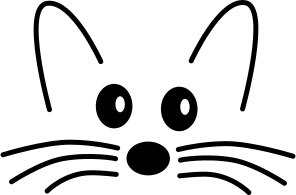
\includegraphics[width=1.4em]{squeak-logo}}}
\newcommand{\dothis}[1]{%
	\medskip
	\noindent\dothisicon
	\ifx#1\empty\else\quad\emph{#1}\fi
	\par\smallskip\nopagebreak}
% NB: To use this in an individual chapter, you must set:
%\graphicspath{{figures/} {../figures/}}
% at the head of the chapter.  Don't forget the final /
%=============================================================
%:Reader hints (hint)
%
% Indicates a non-obvious consequence 
\newcommand{\hint}[1]{\vspace{1ex}\noindent\fbox{\textsc{Astuce}} \emph{#1}}
%=================================================================
% graphics for Morphic handles
\newcommand{\grabHandle}{\raisebox{-0.2ex}{
\includegraphics[width=1em]{blackHandle}}}
\newcommand{\moveHandle}{\raisebox{-0.2ex}{
\includegraphics[width=1em]{moveHandle}}}
\newcommand{\debugHandle}{\raisebox{-0.2ex}{
\includegraphics[width=1em]{debugHandle}}}
% squeak-fr (added for Morphic handles)
\newcommand{\rotateHandle}{\raisebox{-0.2ex}{
\includegraphics[width=1em]{rotateHandle}}}
\newcommand{\viewerHandle}{\raisebox{-0.2ex}{
\includegraphics[width=1em]{viewerHandle}}}
% squeak-fr (add cloverHandle to use \clover in QuickTour.tex as alias
% todo 

%=============================================================
%:Highlighting Important stuff (doublebox)
%
% From Seaside book ...
\newsavebox{\SavedText}
\newlength{\InnerBoxRule}\setlength{\InnerBoxRule}{.75\fboxrule}
\newlength{\OuterBoxRule}\setlength{\OuterBoxRule}{1.5\fboxrule}
\newlength{\BoxSeparation}\setlength{\BoxSeparation}{1.5\fboxrule}
\addtolength{\BoxSeparation}{.5pt}
\newlength{\SaveBoxSep}\setlength{\SaveBoxSep}{2\fboxsep}
%
\newenvironment{doublebox}{\begin{lrbox}{\SavedText}
    \begin{minipage}{.75\textwidth}}
    {\end{minipage}\end{lrbox}\begin{center}
    \setlength{\fboxsep}{\BoxSeparation}\setlength{\fboxrule}{\OuterBoxRule}
    \fbox{\setlength{\fboxsep}{\SaveBoxSep}\setlength{\fboxrule}{\InnerBoxRule}%
      \fbox{\usebox{\SavedText}}}
  \end{center}}
% Use this:
%\newcommand{\important}[1]{\begin{doublebox}#1\end{doublebox}}


\newcommand{\important}[1]{
\noindent\rule{\textwidth}{2pt}\par
\textbf{Important!} #1 \par
\noindent\rule{\textwidth}{2pt}}

\newcommand{\note}[1]{
\noindent\rule{\textwidth}{2pt}\par
\noindent\textbf{Note} #1\par
\noindent\rule{\textwidth}{2pt}}

%=============================================================
%:Section depth
\setcounter{secnumdepth}{2}
%% for this to happen start the file with
%\ifx\wholebook\relax\else
%% $Author$ Martial
% $Date$ Wed Oct 10 13:34:55 CEST 2007
% $Revision$ source: SBE 12715 
% Last Changed Date: 2007-10-08 21:32:45 +0200 (Mon, 08 Oct 2007)
%=============================================================
% NB: documentclass must be set in main document.
% Allows book to be generated in multiple formats.
%=============================================================
%:Packages
%\usepackage[french]{babel}
\usepackage[T1]{fontenc}  %%%%%% really important to get the code directly in the text!
\usepackage{lmodern}
%\usepackage[scaled=0.85]{bookmanx} % needs another scale factor if used with \renewcommand{\sfdefault}{cmbr}
\usepackage{palatino}
%\usepackage[sc]{mathpazo}
%\linespread{1.05}
\usepackage[scaled=0.85]{helvet}
\usepackage{microtype}
\usepackage{graphicx}
\usepackage{theorem}
\usepackage[utf8]{inputenc}
% ON: pdfsync breaks the use of p{width} for tabular columns!
\ifdefined\usepdfsync\usepackage{pdfsync}\fi % Requires texlive 2007
%=============================================================
%:More packages
%Stef should check which ones are used!
%\usepackage{picinpar}
%\usepackage{layout}
%\usepackage{color}
%\definecolor{stefgris}{rgb}{0.85,0.85,0.85}
%\usepackage{enum}
%\usepackage{a4wide}
% \usepackage{fancyhdr}
\usepackage{ifthen}
\usepackage{float}
\usepackage{longtable}
\usepackage{makeidx}
\usepackage[nottoc]{tocbibind}
\usepackage{multicol}
\usepackage{booktabs}	% book-style tables
\usepackage{topcapt}	% enables \topcaption
\usepackage{multirow}
\usepackage{tabularx}
%\usepackage[bottom]{footmisc}
\usepackage{xspace}
\usepackage{alltt}
\usepackage{amssymb,textcomp}
\usepackage[usenames,dvipsnames]{color}
\usepackage{colortbl}
\usepackage[hang]{subfigure}\makeatletter\def\p@subfigure{\thefigure\,}\makeatother
\usepackage{rotating}
\usepackage{enumitem}	% apb: allows more control over tags in enumerations
\usepackage{verbatim}     % for comment environment
\usepackage{varioref}	% for page references that work
\labelformat{footnote}{\thechapter--#1} % to distinguish citations from jurabib
\usepackage{needspace}
\usepackage{isodateo} % enable \isodate
\usepackage[newparttoc]{titlesec}
\usepackage{titletoc}
\usepackage{eurosym}
\usepackage{wrapfig}

\usepackage[
	super,
	citefull=first,
	authorformat={allreversed,and},
	titleformat={commasep,italic}
]{jurabib} % citations as footnotes
\usepackage[
	colorlinks=true,
	linkcolor=black,
	urlcolor=black,
	citecolor=black
]{hyperref}   % should come last

%=============================================================
%:URL style
\makeatletter

\def\url@leostyle{%
  \@ifundefined{selectfont}{\def\UrlFont{\sf}}{\def\UrlFont{\sffamily}}}
% ajouter par Martial pour \traduit (met une dague dans les \doublebox
\def\thempfootnote{\fnsymbol{mpfootnote}}

\makeatother
% Now actually use the newly defined style.
\urlstyle{leo}
%=============================================================
%:Booleans
\newboolean{lulu}
\setboolean{lulu}{false}
\newcommand{\ifluluelse}[2]{\ifthenelse{\boolean{lulu}}{#1}{#2}}
%=============================================================
%:Names
\newcommand{\SUnit}{SUnit\xspace}
\newcommand{\sunit}{SUnit\xspace}
\newcommand{\xUnit}{$x$Unit\xspace}
\newcommand{\JUnit}{JUnit\xspace}
%\newcommand{\XP}{eXtreme Programming\xspace}
\newcommand{\st}{Smalltalk\xspace}
\newcommand{\Squeak}{Squeak\xspace}
\newcommand{\sq}{Squeak\xspace}
\newcommand{\sqmap}{SqueakMap\xspace}
\newcommand{\squeak}{Squeak\xspace}
%\newcommand{\sbe}{\url{scg.unibe.ch/SBE}\xspace}
%\newcommand{\sbe}{\url{squeakbyexample.org}\xspace}
\newcommand{\sbe}{\url{SqueakByExample.org}\xspace}
% squeak-fr: adresse de la version francaise
\newcommand{\spe}{\url{SqueakByExample.org/fr}\xspace}
\newcommand{\sba}{\url{SquareBracketAssociates.org}\xspace}

% squeak-fr: ajout de la \squeakdev pour eviter les problemes de
% changements d'url rencontres dans la VO:
\newcommand{\squeakdev}{\url{www.squeaksource.com/ImageForDevelopers}\xspace} %ou
%\newcommand{\squeakdev}{\url{squeak.ofset.org/squeak-dev}\xspace}

%=============================================================
%:Editorial comment macros
\newcommand{\nnbb}[2]{
    \fbox{\bfseries\sffamily\scriptsize#1}
    {\sf\small$\blacktriangleright$\textit{#2}$\blacktriangleleft$}
   }
\newcommand{\ab}[1]{\nnbb{Andrew}{#1}}
\newcommand{\sd}[1]{\nnbb{St\'{e}f}{#1}}
\newcommand{\md}[1]{\nnbb{Marcus}{#1}}
\newcommand{\on}[1]{\nnbb{Oscar}{#1}}
\newcommand{\damien}[1]{\nnbb{Damien}{#1}}
\newcommand{\lr}[1]{\nnbb{Lukas}{#1}}
\newcommand{\orla}[1]{\nnbb{Orla}{#1}}
%\newcommand{\here}{\nnbb{CONTINUE}{HERE}}
\newcommand{\here}{\nnbb{CONTINUE}{ICI}}

%=============================================================
%:Abbreviation macros
\newcommand{\ie}{\emph{c-\`a-d.}\xspace}
\newcommand{\cad}{\emph{c-\`a-d.}\xspace}
%\newcommand{\eg}{\emph{e.g.},\xspace}
\newcommand{\eg}{\emph{par ex.},\xspace}
\newcommand{\parex}{\emph{par ex.},\xspace}
\newcommand{\etc}{etc\xspace}
%=============================================================
%:Cross reference macros

% [squeak-fr] martial: remarquez les articles devant les noms
\newcommand{\charef}[1]{le chapitre~\ref{cha:#1}\xspace}
% note de martial: utilise dans chapitre Syntax.tex: a redefinir
\newcommand{\charefs}[2]{les chapitres~\ref{cha:#1} et \ref{cha:#2}\xspace}
\newcommand{\secref}[1]{la section~\ref{sec:#1}\xspace}
\newcommand{\figref}[1]{la figure~\ref{fig:#1}\xspace}
\newcommand{\Figref}[1]{La figure~\ref{fig:#1}\xspace}
\newcommand{\appref}[1]{l'annexe~\ref{app:#1}\xspace}
\newcommand{\tabref}[1]{la table~\ref{tab:#1}\xspace}
% defini pour le chapitre Messages.tex
\newcommand{\Tabref}[1]{La table~\ref{tab:#1}\xspace}

% APB: I removed trailing \xspace commands from these macros because
% \xspace mostly doesn't work.  If you want a space after your
% references, type one!
% ON: xspace has always worked just fine for me!  Please leave them in.
%
\newcommand{\ruleref}[1]{\ref{rule:#1}\xspace}
%
\newcommand{\egref}[1]{exemple~\ref{eg:#1}\xspace}
\newcommand{\Egref}[1]{Exemple~\ref{eg:#1}\xspace}
%
\newcommand{\scrref}[1]{script~\ref{scr:#1}\xspace}
\newcommand{\Scrref}[1]{Script~\ref{scr:#1}\xspace}
% t = the
\newcommand{\tscrref}[1]{le script~\ref{scr:#1}\xspace}
\newcommand{\Tscrref}[1]{Le script~\ref{scr:#1}\xspace}
%
\newcommand{\mthref}[1]{m\'ethode~\ref{mth:#1}\xspace}
\newcommand{\mthsref}[1]{m\'ethodes~\ref{mth:#1}\xspace}
\newcommand{\Mthref}[1]{M\'ethode~\ref{mth:#1}\xspace}
\newcommand{\tmthref}[1]{la m\'ethode~\ref{mth:#1}\xspace}
\newcommand{\Tmthref}[1]{La m\'ethode~\ref{mth:#1}\xspace}
%
\newcommand{\clsref}[1]{classe~\ref{cls:#1}\xspace}
\newcommand{\tclsref}[1]{la classe~\ref{cls:#1}\xspace}
\newcommand{\Tclsref}[1]{La classe~\ref{cls:#1}\xspace}
%=============================================================
%:Menu item macro
% for menu items, so we can change our minds on how to print them! (apb)
\definecolor{lightgray}{gray}{0.89}
\newcommand{\menu}[1]{{%
	\setlength{\fboxsep}{0pt}%
	\colorbox{lightgray}{{{\upshape\sffamily\strut \,#1\,}}}}}
% \newcommand{\menu}[1]{{%
% 	\fontfamily{lmr}\selectfont
% 	\upshape\textlangle{\sffamily #1}\textrangle}}
% For submenu items:
\newcommand{\go}{\,$\triangleright$\,}
% \newcommand{\go}{\,$\blacktriangleright$\,}
% For keyboard shortcuts:
%\newcommand{\short}[1]{\mbox{$\langle${\sc CMD}$\rangle$-#1}\xspace}
\newcommand{\short}[1]{\mbox{{\sc cmd}\hspace{0.08em}--\hspace{0.09em}#1}\xspace}
% For buttons:
\newcommand{\button}[1]{{%
	\setlength{\fboxsep}{0pt}%
	\fbox{{\upshape\sffamily\strut \,#1\,}}}}
\newcommand{\toolsflap}{l'onglet \textit{Tools}\xspace}
%=============================================================
%:Reader cues (do this)
%
% Indicate something the reader should try out.
\newcommand{\dothisicon}{\raisebox{-.5ex}{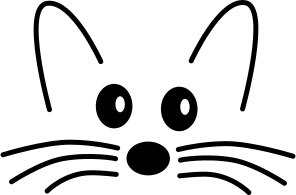
\includegraphics[width=1.4em]{squeak-logo}}}
\newcommand{\dothis}[1]{%
	\medskip
	\noindent\dothisicon
	\ifx#1\empty\else\quad\emph{#1}\fi
	\par\smallskip\nopagebreak}
% NB: To use this in an individual chapter, you must set:
%\graphicspath{{figures/} {../figures/}}
% at the head of the chapter.  Don't forget the final /
%=============================================================
%:Reader hints (hint)
%
% Indicates a non-obvious consequence 
\newcommand{\hint}[1]{\vspace{1ex}\noindent\fbox{\textsc{Astuce}} \emph{#1}}
%=================================================================
% graphics for Morphic handles
\newcommand{\grabHandle}{\raisebox{-0.2ex}{
\includegraphics[width=1em]{blackHandle}}}
\newcommand{\moveHandle}{\raisebox{-0.2ex}{
\includegraphics[width=1em]{moveHandle}}}
\newcommand{\debugHandle}{\raisebox{-0.2ex}{
\includegraphics[width=1em]{debugHandle}}}
% squeak-fr (added for Morphic handles)
\newcommand{\rotateHandle}{\raisebox{-0.2ex}{
\includegraphics[width=1em]{rotateHandle}}}
\newcommand{\viewerHandle}{\raisebox{-0.2ex}{
\includegraphics[width=1em]{viewerHandle}}}
% squeak-fr (add cloverHandle to use \clover in QuickTour.tex as alias
% todo 

%=============================================================
%:Highlighting Important stuff (doublebox)
%
% From Seaside book ...
\newsavebox{\SavedText}
\newlength{\InnerBoxRule}\setlength{\InnerBoxRule}{.75\fboxrule}
\newlength{\OuterBoxRule}\setlength{\OuterBoxRule}{1.5\fboxrule}
\newlength{\BoxSeparation}\setlength{\BoxSeparation}{1.5\fboxrule}
\addtolength{\BoxSeparation}{.5pt}
\newlength{\SaveBoxSep}\setlength{\SaveBoxSep}{2\fboxsep}
%
\newenvironment{doublebox}{\begin{lrbox}{\SavedText}
    \begin{minipage}{.75\textwidth}}
    {\end{minipage}\end{lrbox}\begin{center}
    \setlength{\fboxsep}{\BoxSeparation}\setlength{\fboxrule}{\OuterBoxRule}
    \fbox{\setlength{\fboxsep}{\SaveBoxSep}\setlength{\fboxrule}{\InnerBoxRule}%
      \fbox{\usebox{\SavedText}}}
  \end{center}}
% Use this:
%\newcommand{\important}[1]{\begin{doublebox}#1\end{doublebox}}


\newcommand{\important}[1]{
\noindent\rule{\textwidth}{2pt}\par
\textbf{Important!} #1 \par
\noindent\rule{\textwidth}{2pt}}

\newcommand{\note}[1]{
\noindent\rule{\textwidth}{2pt}\par
\noindent\textbf{Note} #1\par
\noindent\rule{\textwidth}{2pt}}

%=============================================================
%:Section depth
\setcounter{secnumdepth}{2}
%% for this to happen start the file with
%\ifx\wholebook\relax\else
%% $Author$ Martial
% $Date$ Wed Oct 10 13:34:55 CEST 2007
% $Revision$ source: SBE 12715 
% Last Changed Date: 2007-10-08 21:32:45 +0200 (Mon, 08 Oct 2007)
%=============================================================
% NB: documentclass must be set in main document.
% Allows book to be generated in multiple formats.
%=============================================================
%:Packages
%\usepackage[french]{babel}
\usepackage[T1]{fontenc}  %%%%%% really important to get the code directly in the text!
\usepackage{lmodern}
%\usepackage[scaled=0.85]{bookmanx} % needs another scale factor if used with \renewcommand{\sfdefault}{cmbr}
\usepackage{palatino}
%\usepackage[sc]{mathpazo}
%\linespread{1.05}
\usepackage[scaled=0.85]{helvet}
\usepackage{microtype}
\usepackage{graphicx}
\usepackage{theorem}
\usepackage[utf8]{inputenc}
% ON: pdfsync breaks the use of p{width} for tabular columns!
\ifdefined\usepdfsync\usepackage{pdfsync}\fi % Requires texlive 2007
%=============================================================
%:More packages
%Stef should check which ones are used!
%\usepackage{picinpar}
%\usepackage{layout}
%\usepackage{color}
%\definecolor{stefgris}{rgb}{0.85,0.85,0.85}
%\usepackage{enum}
%\usepackage{a4wide}
% \usepackage{fancyhdr}
\usepackage{ifthen}
\usepackage{float}
\usepackage{longtable}
\usepackage{makeidx}
\usepackage[nottoc]{tocbibind}
\usepackage{multicol}
\usepackage{booktabs}	% book-style tables
\usepackage{topcapt}	% enables \topcaption
\usepackage{multirow}
\usepackage{tabularx}
%\usepackage[bottom]{footmisc}
\usepackage{xspace}
\usepackage{alltt}
\usepackage{amssymb,textcomp}
\usepackage[usenames,dvipsnames]{color}
\usepackage{colortbl}
\usepackage[hang]{subfigure}\makeatletter\def\p@subfigure{\thefigure\,}\makeatother
\usepackage{rotating}
\usepackage{enumitem}	% apb: allows more control over tags in enumerations
\usepackage{verbatim}     % for comment environment
\usepackage{varioref}	% for page references that work
\labelformat{footnote}{\thechapter--#1} % to distinguish citations from jurabib
\usepackage{needspace}
\usepackage{isodateo} % enable \isodate
\usepackage[newparttoc]{titlesec}
\usepackage{titletoc}
\usepackage{eurosym}
\usepackage{wrapfig}

\usepackage[
	super,
	citefull=first,
	authorformat={allreversed,and},
	titleformat={commasep,italic}
]{jurabib} % citations as footnotes
\usepackage[
	colorlinks=true,
	linkcolor=black,
	urlcolor=black,
	citecolor=black
]{hyperref}   % should come last

%=============================================================
%:URL style
\makeatletter

\def\url@leostyle{%
  \@ifundefined{selectfont}{\def\UrlFont{\sf}}{\def\UrlFont{\sffamily}}}
% ajouter par Martial pour \traduit (met une dague dans les \doublebox
\def\thempfootnote{\fnsymbol{mpfootnote}}

\makeatother
% Now actually use the newly defined style.
\urlstyle{leo}
%=============================================================
%:Booleans
\newboolean{lulu}
\setboolean{lulu}{false}
\newcommand{\ifluluelse}[2]{\ifthenelse{\boolean{lulu}}{#1}{#2}}
%=============================================================
%:Names
\newcommand{\SUnit}{SUnit\xspace}
\newcommand{\sunit}{SUnit\xspace}
\newcommand{\xUnit}{$x$Unit\xspace}
\newcommand{\JUnit}{JUnit\xspace}
%\newcommand{\XP}{eXtreme Programming\xspace}
\newcommand{\st}{Smalltalk\xspace}
\newcommand{\Squeak}{Squeak\xspace}
\newcommand{\sq}{Squeak\xspace}
\newcommand{\sqmap}{SqueakMap\xspace}
\newcommand{\squeak}{Squeak\xspace}
%\newcommand{\sbe}{\url{scg.unibe.ch/SBE}\xspace}
%\newcommand{\sbe}{\url{squeakbyexample.org}\xspace}
\newcommand{\sbe}{\url{SqueakByExample.org}\xspace}
% squeak-fr: adresse de la version francaise
\newcommand{\spe}{\url{SqueakByExample.org/fr}\xspace}
\newcommand{\sba}{\url{SquareBracketAssociates.org}\xspace}

% squeak-fr: ajout de la \squeakdev pour eviter les problemes de
% changements d'url rencontres dans la VO:
\newcommand{\squeakdev}{\url{www.squeaksource.com/ImageForDevelopers}\xspace} %ou
%\newcommand{\squeakdev}{\url{squeak.ofset.org/squeak-dev}\xspace}

%=============================================================
%:Editorial comment macros
\newcommand{\nnbb}[2]{
    \fbox{\bfseries\sffamily\scriptsize#1}
    {\sf\small$\blacktriangleright$\textit{#2}$\blacktriangleleft$}
   }
\newcommand{\ab}[1]{\nnbb{Andrew}{#1}}
\newcommand{\sd}[1]{\nnbb{St\'{e}f}{#1}}
\newcommand{\md}[1]{\nnbb{Marcus}{#1}}
\newcommand{\on}[1]{\nnbb{Oscar}{#1}}
\newcommand{\damien}[1]{\nnbb{Damien}{#1}}
\newcommand{\lr}[1]{\nnbb{Lukas}{#1}}
\newcommand{\orla}[1]{\nnbb{Orla}{#1}}
%\newcommand{\here}{\nnbb{CONTINUE}{HERE}}
\newcommand{\here}{\nnbb{CONTINUE}{ICI}}

%=============================================================
%:Abbreviation macros
\newcommand{\ie}{\emph{c-\`a-d.}\xspace}
\newcommand{\cad}{\emph{c-\`a-d.}\xspace}
%\newcommand{\eg}{\emph{e.g.},\xspace}
\newcommand{\eg}{\emph{par ex.},\xspace}
\newcommand{\parex}{\emph{par ex.},\xspace}
\newcommand{\etc}{etc\xspace}
%=============================================================
%:Cross reference macros

% [squeak-fr] martial: remarquez les articles devant les noms
\newcommand{\charef}[1]{le chapitre~\ref{cha:#1}\xspace}
% note de martial: utilise dans chapitre Syntax.tex: a redefinir
\newcommand{\charefs}[2]{les chapitres~\ref{cha:#1} et \ref{cha:#2}\xspace}
\newcommand{\secref}[1]{la section~\ref{sec:#1}\xspace}
\newcommand{\figref}[1]{la figure~\ref{fig:#1}\xspace}
\newcommand{\Figref}[1]{La figure~\ref{fig:#1}\xspace}
\newcommand{\appref}[1]{l'annexe~\ref{app:#1}\xspace}
\newcommand{\tabref}[1]{la table~\ref{tab:#1}\xspace}
% defini pour le chapitre Messages.tex
\newcommand{\Tabref}[1]{La table~\ref{tab:#1}\xspace}

% APB: I removed trailing \xspace commands from these macros because
% \xspace mostly doesn't work.  If you want a space after your
% references, type one!
% ON: xspace has always worked just fine for me!  Please leave them in.
%
\newcommand{\ruleref}[1]{\ref{rule:#1}\xspace}
%
\newcommand{\egref}[1]{exemple~\ref{eg:#1}\xspace}
\newcommand{\Egref}[1]{Exemple~\ref{eg:#1}\xspace}
%
\newcommand{\scrref}[1]{script~\ref{scr:#1}\xspace}
\newcommand{\Scrref}[1]{Script~\ref{scr:#1}\xspace}
% t = the
\newcommand{\tscrref}[1]{le script~\ref{scr:#1}\xspace}
\newcommand{\Tscrref}[1]{Le script~\ref{scr:#1}\xspace}
%
\newcommand{\mthref}[1]{m\'ethode~\ref{mth:#1}\xspace}
\newcommand{\mthsref}[1]{m\'ethodes~\ref{mth:#1}\xspace}
\newcommand{\Mthref}[1]{M\'ethode~\ref{mth:#1}\xspace}
\newcommand{\tmthref}[1]{la m\'ethode~\ref{mth:#1}\xspace}
\newcommand{\Tmthref}[1]{La m\'ethode~\ref{mth:#1}\xspace}
%
\newcommand{\clsref}[1]{classe~\ref{cls:#1}\xspace}
\newcommand{\tclsref}[1]{la classe~\ref{cls:#1}\xspace}
\newcommand{\Tclsref}[1]{La classe~\ref{cls:#1}\xspace}
%=============================================================
%:Menu item macro
% for menu items, so we can change our minds on how to print them! (apb)
\definecolor{lightgray}{gray}{0.89}
\newcommand{\menu}[1]{{%
	\setlength{\fboxsep}{0pt}%
	\colorbox{lightgray}{{{\upshape\sffamily\strut \,#1\,}}}}}
% \newcommand{\menu}[1]{{%
% 	\fontfamily{lmr}\selectfont
% 	\upshape\textlangle{\sffamily #1}\textrangle}}
% For submenu items:
\newcommand{\go}{\,$\triangleright$\,}
% \newcommand{\go}{\,$\blacktriangleright$\,}
% For keyboard shortcuts:
%\newcommand{\short}[1]{\mbox{$\langle${\sc CMD}$\rangle$-#1}\xspace}
\newcommand{\short}[1]{\mbox{{\sc cmd}\hspace{0.08em}--\hspace{0.09em}#1}\xspace}
% For buttons:
\newcommand{\button}[1]{{%
	\setlength{\fboxsep}{0pt}%
	\fbox{{\upshape\sffamily\strut \,#1\,}}}}
\newcommand{\toolsflap}{l'onglet \textit{Tools}\xspace}
%=============================================================
%:Reader cues (do this)
%
% Indicate something the reader should try out.
\newcommand{\dothisicon}{\raisebox{-.5ex}{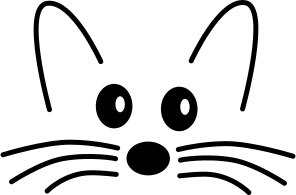
\includegraphics[width=1.4em]{squeak-logo}}}
\newcommand{\dothis}[1]{%
	\medskip
	\noindent\dothisicon
	\ifx#1\empty\else\quad\emph{#1}\fi
	\par\smallskip\nopagebreak}
% NB: To use this in an individual chapter, you must set:
%\graphicspath{{figures/} {../figures/}}
% at the head of the chapter.  Don't forget the final /
%=============================================================
%:Reader hints (hint)
%
% Indicates a non-obvious consequence 
\newcommand{\hint}[1]{\vspace{1ex}\noindent\fbox{\textsc{Astuce}} \emph{#1}}
%=================================================================
% graphics for Morphic handles
\newcommand{\grabHandle}{\raisebox{-0.2ex}{
\includegraphics[width=1em]{blackHandle}}}
\newcommand{\moveHandle}{\raisebox{-0.2ex}{\includegraphics[width=1em]{moveHandle}}}
\newcommand{\debugHandle}{\raisebox{-0.2ex}{\includegraphics[width=1em]{debugHandle}}}
% squeak-fr (added for Morphic handles)
\newcommand{\rotateHandle}{\raisebox{-0.2ex}{\includegraphics[width=1em]{rotateHandle}}}
\newcommand{\viewerHandle}{\raisebox{-0.2ex}{\includegraphics[width=1em]{viewerHandle}}}
% squeak-fr (add cloverHandle to use \clover in QuickTour.tex as alias
% todo 

%=============================================================
%:Highlighting Important stuff (doublebox)
%
% From Seaside book ...
\newsavebox{\SavedText}
\newlength{\InnerBoxRule}\setlength{\InnerBoxRule}{.75\fboxrule}
\newlength{\OuterBoxRule}\setlength{\OuterBoxRule}{1.5\fboxrule}
\newlength{\BoxSeparation}\setlength{\BoxSeparation}{1.5\fboxrule}
\addtolength{\BoxSeparation}{.5pt}
\newlength{\SaveBoxSep}\setlength{\SaveBoxSep}{2\fboxsep}
%
\newenvironment{doublebox}{\begin{lrbox}{\SavedText}
    \begin{minipage}{.75\textwidth}}
    {\end{minipage}\end{lrbox}\begin{center}
    \setlength{\fboxsep}{\BoxSeparation}\setlength{\fboxrule}{\OuterBoxRule}
    \fbox{\setlength{\fboxsep}{\SaveBoxSep}\setlength{\fboxrule}{\InnerBoxRule}%
      \fbox{\usebox{\SavedText}}}
  \end{center}}
% Use this:
%\newcommand{\important}[1]{\begin{doublebox}#1\end{doublebox}}


\newcommand{\important}[1]{
\noindent\rule{\textwidth}{2pt}\par
\textbf{Important!} #1 \par
\noindent\rule{\textwidth}{2pt}}

\newcommand{\note}[1]{
\noindent\rule{\textwidth}{2pt}\par
\noindent\textbf{Note} #1\par
\noindent\rule{\textwidth}{2pt}}

%=============================================================
%:Section depth
\setcounter{secnumdepth}{2}
%% for this to happen start the file with
%\ifx\wholebook\relax\else
%\input{../common.tex}
%\begin{document}
%\fi
% and terminate by
% \ifx\wholebook\relax\else\end{document}\fi

\DeclareGraphicsExtensions{.pdf, .jpg, .png}
%=============================================================
%:PDF setup
\hypersetup{
%   a4paper,
%   pdfstartview=FitV,
%   colorlinks,
%   linkcolor=darkblue,
%   citecolor=darkblue,
%   pdftitle={Squeak by Example},
pdftitle={Squeak par l'exemple},
   pdfauthor={Andrew Black, St\'ephane Ducasse,	Oscar Nierstrasz,
Damien Pollet},
   pdfkeywords={Smalltalk, Squeak, Programmation Orient\'ee Objet},
pdfsubject={Informatique, Computer Science}
}
%=============================================================
%:Page layout and appearance
%
% \renewcommand{\headrulewidth}{0pt}
\renewcommand{\chaptermark}[1]{\markboth{#1}{}}
\renewcommand{\sectionmark}[1]{\markright{\thesection\ #1}}
\renewpagestyle{plain}[\small\itshape]{%
	\setheadrule{0pt}%
	\sethead[][][]{}{}{}%
	\setfoot[][][]{}{}{}}
\renewpagestyle{headings}[\small\itshape]{%
	\setheadrule{0pt}%
	\setmarks{chapter}{section}%
	\sethead[\thepage][][\chaptertitle]{\sectiontitle}{}{\thepage}%
	\setfoot[][][]{}{}{}}
% pagestyle for tableofcontents + index (martial: 2008/04/23)
\newpagestyle{newheadings}[\small\itshape]{%
	\setheadrule{0pt}%
	\setmarks{chapter}{section}%
	\sethead[\thepage][][\chaptertitle]{\chaptertitle}{}{\thepage}%
	\setfoot[][][]{}{}{}}
%=============================================================
%:Title section setup and TOC numbering depth
\setcounter{secnumdepth}{1}
\setcounter{tocdepth}{1}
\titleformat{\part}[display]{\centering}{\huge\partname\ \thepart}{1em}{\Huge\textbf}[]
\titleformat{\chapter}[display]{}{\huge\chaptertitlename\ \thechapter}{1em}{\Huge\raggedright\textbf}[]
\titlecontents{part}[3pc]{%
		\pagebreak[2]\addvspace{1em plus.4em minus.2em}%
		\leavevmode\large\bfseries}
	{\contentslabel{3pc}}{\hspace*{-3pc}}
	{}[\nopagebreak]
\titlecontents{chapter}[3pc]{%
		\pagebreak[0]\addvspace{1em plus.2em minus.2em}%
		\leavevmode\bfseries}
	{\contentslabel{3pc}}{}
	{\hfill\contentspage}[\nopagebreak]
\dottedcontents{section}[3pc]{}{3pc}{1pc}
\dottedcontents{subsection}[3pc]{}{0pc}{1pc}
% \dottedcontents{subsection}[4.5em]{}{0pt}{1pc}
% Make \cleardoublepage insert really blank pages http://www.tex.ac.uk/cgi-bin/texfaq2html?label=reallyblank
\let\origdoublepage\cleardoublepage
\newcommand{\clearemptydoublepage}{%
  \clearpage
  {\pagestyle{empty}\origdoublepage}}
\let\cleardoublepage\clearemptydoublepage % see http://www.tex.ac.uk/cgi-bin/texfaq2html?label=patch
%=============================================================
%:FAQ macros (for FAQ chapter)
\newtheorem{faq}{FAQ}
\newcommand{\answer}{\paragraph{R\'eponse}\ }
%=============================================================
%:Listings package configuration
\usepackage{listings}
\newcommand{\caret}{\makebox{\raisebox{0.4ex}{\footnotesize{$\wedge$}}}}
\lstdefinelanguage{Smalltalk}{
%  morekeywords={self,super,true,false,nil,thisContext}, % This is overkill
  morestring=[d]',
  morecomment=[s]{"}{"},
  alsoletter={\#:},
  escapechar={!},
  escapebegin=\itshape, % comment-like by default (Martial 11/2007)
  literate=
    {BANG}{!}1
    {UNDERSCORE}{\_}1
    {\\st}{Smalltalk}9 % convenience -- in case \st occurs in code
    % {'}{{\textquotesingle}}1 % replaced by upquote=true in \lstset
    {_}{{$\leftarrow$}}1
    {>>>}{{\sep}}1
    {^}{{$\uparrow$}}1
    {~}{{$\sim$}}1
    {-}{{\sf -\hspace{-0.13em}-}}1  % the goal is to make - the same width as +
    {+}{\raisebox{0.08ex}{+}}1		% and to raise + off the baseline to match -
    {-->}{{\quad$\longrightarrow$\quad}}3
	, % Don't forget the comma at the end!
  tabsize=4
}[keywords,comments,strings]
% ajout pour les échappements dans les codes
% indispensable pour mettre le code en emphase (cf. Model.tex) 
\newcommand{\codeify}[1]{\NoAutoSpaceBeforeFDP#1\AutoSpaceBeforeFDP}
\newcommand{\normcomment}[1]{\emph{#1}} %cf. Streams
\newcommand{\normcode}[1]{\emph{\codeify{#1}}} %cf. Streams
\newcommand{\emcode}[1]{\textbf{\normcode{#1}}} % Martial 11/2007
\lstset{language=Smalltalk,
	basicstyle=\sffamily,
	keywordstyle=\color{black}\bfseries,
	% stringstyle=\ttfamily, % Ugly! do we really want this? -- on
	%commentstyle=\itshape,
	mathescape=true,
	showstringspaces=false,
	keepspaces=true,
	breaklines=true,
	breakautoindent=true,
	lineskip={-1pt}, % Ugly hack
	upquote=true, % straight quote; requires textcomp package
	columns=fullflexible} % no fixed width fonts
% In-line code (literal)
% Normally use this for all in-line code:
\newcommand{\ct}{\lstinline[mathescape=false,basicstyle={\sffamily\upshape}]}
% apb 2007.8.28 added the \upshape declaration to avoid getting italicized code in \dothis{ } sections.
% In-line code (latex enabled)
% Use this only in special situations where \ct does not work
% (within section headings ...):

% [squeak-fr] Modification de \lct suivant les indications de Martial Boniou
\newcommand{\lct}[1]{\textsf{\textup{\NoAutoSpaceBeforeFDP #1
\AutoSpaceBeforeFDP}}} %\xspace

% Use these for system categories and protocols:
\newcommand{\scat}[1]{\emph{\textsf{#1}}\xspace}
\newcommand{\pkg}[1]{\emph{\textsf{#1}}\xspace}
\newcommand{\prot}[1]{\emph{\textsf{#1}}\xspace}
% Code environments
% NB: the arg is for tests
% Only code and example environments may be tests
\lstnewenvironment{code}[1]{%
	\lstset{%
		frame=lines,
		mathescape=false
	}
}{}
\def\ignoredollar#1{}
%=============================================================
%:Code environments (method, script ...)
% NB: the third arg is for tests
% Only code and example environments may be tests
\lstnewenvironment{example}[3][defaultlabel]{%
	\renewcommand{\lstlistingname}{Exemple}%
	\lstset{
		frame=lines,
		mathescape=false,
		caption={\emph{#2}},
		label={eg:#1}
	}
}{}
\lstnewenvironment{script}[2][defaultlabel]{%
\renewcommand{\lstlistingname}{Script}%
	\lstset{
		frame=lines,
		mathescape=false,
		name={Script},
		caption={\emph{#2}},
		label={scr:#1}
	}
}{}
%I could not find a way yo get the Experiment #numb followed by the caption in a black box
%\colorbox{black}{\makebox[\textwidth]{  \color{white} {\large {\bfseries Experiment 3-1 (crear i moure un robot)}} }}
\lstnewenvironment{experiment}[2][defaultlabel]{%
%\noindent\rule{\textwidth}{2pt}\vspace{-0.8cm}
\renewcommand{\lstlistingname}{Experiment}%
	\lstset{
		frame=none,
		rulecolor=\color{black},
		mathescape=false,
		name={Experiment},
		caption={\emph{#2}},
		label={scr:#1}
	}
}{%\vspace{-0.5cm}\noindent\rule{\textwidth}{2pt}
}

\lstnewenvironment{method}[2][defaultlabel]{%
	\renewcommand{\lstlistingname}{Method}%
	\lstset{
		frame=lines,
		mathescape=false,
		name={M\'ethode},
		caption={\emph{#2}},
		label={mth:#1}
	}
}{}
\lstnewenvironment{methods}[2][defaultlabel]{% just for multiple methods at once
	\renewcommand{\lstlistingname}{Methods}%
	\lstset{
		frame=lines,
		mathescape=false,
		name={M\'ethode},
		caption={\emph{#2}},
		label={mth:#1}
	}
}{}
\lstnewenvironment{numMethod}[2][defaultlabel]{%
	\renewcommand{\lstlistingname}{Method}%
	\lstset{
		numbers=left,
		numberstyle={\tiny\sffamily},
		frame=lines,
		mathescape=false,
		name={M\'ethode},
		caption={\emph{#2}},
		label={mth:#1}
	}
}{}
% \lstnewenvironment{classdef}[2][defaultlabel]{%
% 	\renewcommand{\lstlistingname}{Classe}%
% 	\lstset{
% 		frame=lines,
% 		mathescape=false,
% 		name={Classe},
% 		caption={\emph{#2}},
% 		label={cls:#1}
% 	}
% }{}

%%%%%%%%%%%%%%%%%%%%%%%%%%%%%%%%%%%%%%%%%%%%%%%%%%%%%%%%%%%%%%%%%%%%%%%%%%%%%%%%%%%%%%%%%%%%%%%%%
%%From the original book latex template
%%%%%%%%%%%%%%%%%%%%%%%%%%%%%%%%%%%%%%%%%%%%%%%%%%%%%%%%%%%%%%%%%%%%%%%%%%%%%%%%%%%%%%%%%%%%%%%%%
\theoremstyle{break}
{\theorembodyfont{\rmfamily}\theoremstyle{break}
\newtheorem{privScript}{Script}[chapter]
%\newtheorem{privMethod}{Method}[chapter]
\newtheorem{privExercise}{Experiment}[chapter]}

% \theoremstyle{break}
% {\theorembodyfont{\rmfamily} \newtheorem{privMethod}{Method}[chapter]}

%class
\theoremstyle{break}
{\theorembodyfont{\rmfamily} \newtheorem{privClassDef}{Class}[chapter]}

%important
\theoremstyle{break}
{\theorembodyfont{\rmfamily} \newtheorem{privTemplate}{Important Messages}[chapter]}

% experiment
\newenvironment{exercise}
    {\begin{privExercise}\mbox{}\\}
    {\end{privExercise}}


%%% for figure
\newsavebox{\ScriptFigure}
\newlength{\ScriptWidth}
\newlength{\FigureWidth}

%%%%%%%%%%%%%%%%%%%%%%%%%%%%%%%%%%%%%%%%%%%%%%%%%%%%%%%%%%%%%%%%%%%%%%%%%%%%%%%%
\newenvironment{scriptfig}[3][0.6]
   {\setlength{\ScriptWidth}{\linewidth*\real{#1}}%
   \setlength{\FigureWidth}{\linewidth-(\linewidth*\real{#1})}%
   \savebox{\ScriptFigure}%
	{\parbox{\FigureWidth}{\includegraphics[width=0.98\FigureWidth]{#2}}}%
   \par\noindent\begin{minipage}{\linewidth}\hrule\vskip 0.2cm\begin{minipage}[c]{\ScriptWidth}%
   \begin{stefscript}[{\em #3}]\begin{alltt}\sffamily}
   {\end{alltt}\end{stefscript}\end{minipage}\hfill
   \usebox{\ScriptFigure}
   \vskip 1ex\hrule\end{minipage}\vskip 1ex\par}

%%%%%%%%%%%%%%%%%%%%%%%%%%%%%%%%%%%%%%%%%%%%%%%%%%%%%%%%%%%%%%%%%%%%%%%%%%%%%%%%
%% to be able to specify the complete set of values for includegraphics
%% may be will be changed but not the interface
\newenvironment{scriptfigwithsize}[3][0.6]
   {\setlength{\ScriptWidth}{\linewidth*\real{#1}}%
   \setlength{\FigureWidth}{\linewidth-(\linewidth*\real{#1})}%
   \savebox{\ScriptFigure}{\parbox{\FigureWidth}{\raggedleft{#2}}}%
   \par\noindent\begin{minipage}{\linewidth}\hrule\vskip 0.3cm\begin{minipage}[c]{\ScriptWidth}%
   \begin{stefscript}[{\em #3}]\begin{alltt}\sffamily}
   {\end{alltt}\end{stefscript}\end{minipage}\hfill
   \usebox{\ScriptFigure}
   \vskip 1ex\hrule\end{minipage}\vskip 1ex\par}

% \newenvironment{methodfig}[2][0.6]
%    {\setlength{\ScriptWidth}{\linewidth*\real{#1}}%
%    \setlength{\FigureWidth}{\linewidth-(\linewidth*\real{#1})}%
%    \savebox{\ScriptFigure}{\parbox{\FigureWidth}{\includegraphics[width=.98\FigureWidth]{#2}}}%
%    \par\noindent\rule{\linewidth}{1mm}
%    \\[-0.3cm]\noindent\rule{\linewidth}{0.1mm}
%    \noindent\begin{minipage}[c]{\ScriptWidth}\begin{privMethod}\begin{alltt}\sffamily}
%    {\end{alltt}\end{privMethod}\end{minipage}\hfill
%    \usebox{\ScriptFigure} \vskip 1ex\hrule\vskip 1ex\par}

% \newenvironment{method}
% {\par\noindent\begin{minipage}{\linewidth}\vspace{0.2cm}\begin{privMethod}\begin{nminipage}\vspace{-0.2cm}\rule{\linewidth}{1mm}\\[-0.6cm]\rule{\linewidth}{0.1mm}\end{nminipage}\hspace*{\scriptindent}\codesize\begin{nalltt}\vspace{-0.2cm}}
% {\end{nalltt}\normalsize\vspace{-0.1cm}\hrule\end{privMethod}\vspace{0.2cm}\end{minipage}}


% \newenvironment{classdef}
% {\par\noindent\begin{minipage}{\linewidth}\vspace{0.2cm}\begin{privClassDef}\begin{nminipage}\vspace{-0.2cm}\rule{\linewidth}{1mm}\\[-0.6cm]\rule{\linewidth}{0.1mm}\end{nminipage}\hspace*{\scriptindent}\codesize\begin{nalltt}\vspace{-0.2cm}}
% {\end{nalltt}\normalsize\vspace{-0.1cm}\hrule\end{privClassDef}\vspace{0.2cm}\end{minipage}}


% \newenvironment{template}
% {\par\noindent\begin{minipage}{\linewidth}\vspace{0.3cm}\begin{privTemplate}\begin{nminipage}\vspace{-0.4cm}\rule{\linewidth}{0.1mm}\end{nminipage}\hspace*{\scriptindent}\begin{nalltt}\vspace{-0.7cm}}
% {\end{nalltt}\vspace{-0.1cm}\hrule\end{privTemplate}\end{minipage}\vspace{0.3cm}}

\newenvironment{exofig}[2][0.7]
   {\setlength{\ScriptWidth}{\linewidth*\real{#1}}
   \setlength{\FigureWidth}{\linewidth-(\linewidth*\real{#1})}
   \savebox{\ScriptFigure}{\parbox{\FigureWidth}{\raggedleft{\includegraphics[width=.98\FigureWidth]{#2}}}}
   \par\noindent\begin{minipage}{\linewidth}\hrule\vskip 0.3cm\begin{minipage}[c]{\ScriptWidth}%
   \begin{privExercise}}
   {\end{privExercise}\end{minipage}\hfill
   \usebox{\ScriptFigure}
   \vskip 1ex\hrule\end{minipage}\vskip 1ex\par}

\newenvironment{exofigwithsize}[2][0.7]
   {\setlength{\ScriptWidth}{\linewidth*\real{#1}}
   \setlength{\FigureWidth}{\linewidth-(\linewidth*\real{#1})}
   \savebox{\ScriptFigure}{\parbox{\FigureWidth}{\raggedleft{#2}}}
   \par\noindent\begin{minipage}{\linewidth}\hrule\vskip 0.3cm\begin{minipage}[c]{\ScriptWidth}%
   \begin{privExercise}}
   {\end{privExercise}\end{minipage}\hfill\usebox{\ScriptFigure}
   \vskip 1ex\hrule\end{minipage}\vskip 1ex\par}

\newenvironment{exofigwithsizeandtitle}[3][0.7]
   {\setlength{\ScriptWidth}{\linewidth*\real{#1}}
   \setlength{\FigureWidth}{\linewidth-(\linewidth*\real{#1})}
   \savebox{\ScriptFigure}{\parbox{\FigureWidth}{\raggedleft{#2}}}
   \vskip 0.3cm\par\noindent\begin{minipage}{\linewidth}\hrule\vskip 0.1cm\begin{minipage}[c]{\ScriptWidth}%
   \begin{privExercise}[\em{#3}]}
   {\end{privExercise}\end{minipage}\hfill\usebox{\ScriptFigure}
   \vskip 1ex\hrule\end{minipage}\vskip 1ex\par}

\newenvironment{exofigwithtitle}[3][0.7]
   {\setlength{\ScriptWidth}{\linewidth*\real{#1}}
   \setlength{\FigureWidth}{\linewidth-(\linewidth*\real{#1})}
   \savebox{\ScriptFigure}{\parbox{\FigureWidth}{\raggedleft{\includegraphics[width=.98\FigureWidth]{#2}}}}
   \par\noindent\begin{minipage}{\linewidth}\hrule\vskip 0.3cm\begin{minipage}[c]{\ScriptWidth}%
   \begin{privExercise}[\em{#3}]}
   {\end{privExercise}\end{minipage}\hfill
   \usebox{\ScriptFigure}
   \vskip 1ex\hrule\end{minipage}\vskip 1ex\par}


\newenvironment{exonofigwithtitle}[3][0.7]
   {\setlength{\ScriptWidth}{\linewidth*\real{#1}}
   \setlength{\FigureWidth}{\linewidth-(\linewidth*\real{#1})}
   \savebox{\ScriptFigure}{\parbox{\FigureWidth}{\raggedleft{\includegraphics[width=.98\FigureWidth]{#2}}}}
   \par\noindent\begin{minipage}{\linewidth}\hrule\vskip 0.3cm\begin{minipage}[c]{\ScriptWidth}%
   \begin{privExercise}[\em{#3}]}
   {\end{privExercise}\end{minipage}\hfill
   \usebox{\ScriptFigure}
   \vskip 1ex\hrule\end{minipage}\vskip 1ex\par}

\newenvironment{exonofig}
   {\par\noindent\begin{minipage}[t]{\linewidth}\noindent\begin{privExercise}}
   {\end{privExercise}\end{minipage}\vspace{0.5cm}\par}

\newenvironment{exonofigtitle}[1]
   {\par\noindent\begin{minipage}[t]{\linewidth}\noindent\begin{privExercise}[\em{#1}]}
   {\end{privExercise}\end{minipage}\vspace{0.5cm}\par}
		
% \newenvironment{solfig}[3][0.5]
%    {\setlength{\ScriptWidth}{\linewidth*\real{#1}}
%    \setlength{\FigureWidth}{\linewidth-\linewidth*\real{#1}}
%    \savebox{\ScriptFigure}{\parbox{\FigureWidth}{\includegraphics[width=.9\linewidth]{#2}}}
%    \par\noindent\vskip 1ex\hrule\vskip 1ex\begin{minipage}[t]{\ScriptWidth}
%    {\bf Solution #3} \begin{alltt}\sffamily}
%    {\end{alltt}\end{minipage}\hfill
%    \usebox{\ScriptFigure}
%    \vskip 1ex\hrule\vskip 1ex\par}
% 
% \newenvironment{solnofig}[1]
%    {\par\noindent\vskip 1ex\hrule\vskip 1ex\begin{minipage}[t]{\ScriptWidth}
%    {\bf Solution #1} \begin{alltt}\sffamily}
%    {\end{alltt}\end{minipage}\hfill
%    \vskip 1ex\hrule\vskip 1ex\par}
% 
% \newenvironment{exoscript}[3][0.5]
%    {\setlength{\ScriptWidth}{\linewidth*\real{#1}}
%     \setlength{\FigureWidth}{\linewidth-\linewidth*\real{#1}}
%     \savebox{\ScriptFigure}{\begin{minipage}\begin{alltt}\sffamily#3\end{alltt}\end{minipage}}
%     \par\noindent\vskip 1ex\hrule\vskip 1ex\begin{minipage}[t]{\ScriptWidth}
%     \begin{privExercise}}
%     {\end{privExercise}\end{minipage}\hfill
%     \usebox{\ScriptFigure}
% \vskip 1ex\hrule\vskip 1ex\par}


%%%%%%%%%%%%%%%%%%%%%%%%%%%%%%%%%%%%%%%%%%%%%%%%%%%%%%%%%%%%%%%%
%% Define the indentation from which the code script starts
%\newlength{\scriptindent}
%\setlength{\scriptindent}{.3cm}
%%%%%%%%%%%%%%%%%%%%%%%%%%%%%%%%%%%%%%%%%%%%%%%%%%%%%%%%%%%%%%%%
%% Method presentation 
%\newlength{\methodindent}
%\newlength{\methodwordlength}
%\newlength{\aftermethod}
%\setlength{\methodindent}{0.2cm}
%\settowidth{\methodwordlength}{\ M\'ethode\ }

%%%%%%%%%%%%%%%%%%%%%%%%%%%%%%%%%%%%%%%%%%%%%%%%%%%%%%%%%%%%%%%%
\theoremstyle{break}
{\theorembodyfont{\rmfamily} \newtheorem{fonction}{Script}[chapter]}

\newsavebox{\fminibox}
\newlength{\fminilength}
% Fait un truc encadre
\newenvironment{fminipage}[1][\linewidth]
  {\setlength{\fminilength}{#1-2\fboxsep-2\fboxrule}
        \begin{lrbox}{\fminibox}\begin{minipage}{\fminilength}}
  { \end{minipage}\end{lrbox}\noindent\fbox{\usebox{\fminibox}}}

% Pareil mais pas encadre (a utiliser pour ne pas couper une fonction en 2)
\newenvironment{nminipage}[1][\linewidth]
  {\setlength{\fminilength}{#1}
        \begin{lrbox}{\fminibox}\begin{minipage}{\fminilength}}
  { \end{minipage}\end{lrbox}\noindent\mbox{\usebox{\fminibox}}}

% Un alltt encadre
\newenvironment{falltt}
  {\vspace*{0.3cm}\begin{fminipage}\begin{alltt}\ttfamily}
  {\end{alltt}\end{fminipage}\vspace*{0.3cm}}

% Un alltt pas encadre
\newenvironment{nalltt}
  {\vspace*{0.3cm}\begin{nminipage}\begin{alltt}\sffamily}
  {\end{alltt}\end{nminipage}\vspace*{0.3cm}}

% Une fonction encadree
\newenvironment{ffonction}[1]
  {\begin{fonction}[#1]\begin{fminipage}\begin{alltt}\ttfamily\rule{\linewidth}{0.5pt}}
{\end{alltt}\end{fminipage}\end{fonction}}


\theoremstyle{break}
{\theorembodyfont{\rmfamily} \newtheorem{stefscript}{Script}[chapter]}

\theoremstyle{break}
{\theorembodyfont{\rmfamily} \newtheorem{exampleScript}{Examples}[chapter]}


%%Not used
\newenvironment{ncscript}[1]
{\vspace{-0.5cm}\begin{stefscript}[#1]\begin{nalltt}\rule{\linewidth}{1.5pt}\vspace{-0.1cm}
\hspace*{\scriptindent}\begin{nalltt}}
{\end{nalltt}\vspace{-0.5cm}\hrule\end{nalltt}\end{stefscript}\vspace{-0.5cm}}
%%Not used
\newenvironment{soluscript}[1]
{\begin{nalltt}\textbf{Solution du script : #1.}\\
\rule{\linewidth}{1.5pt}
\hspace*{\scriptindent}\begin{nalltt}}
{\end{nalltt}\vspace{-0.5cm}\hrule\end{nalltt}\vspace{-0.5cm}\\}




\newenvironment{scriptwithtitle}[1]
{\vspace{-0.3cm}\begin{stefscript}[{\em #1}]\begin{nalltt}\rule{\linewidth}{1.5pt}\vspace{-0.3cm}\hspace*{\scriptindent}\begin{nalltt}\codesize}
{\normalsize\end{nalltt}\vspace{-0.2cm}\hrule\end{nalltt}\end{stefscript}\vspace{-0.5cm}}

\newenvironment{scriptwithouttitle}
{\vspace{-0.5cm}\begin{stefscript}\codesize\begin{nalltt}\rule{\linewidth}{1.5pt}\vspace{-0.1cm}
\hspace*{\scriptindent}\begin{nalltt}}
{\end{nalltt}\vspace{-0.5cm}\hrule\end{nalltt}\normalsize\end{stefscript}\vspace{-0.5cm}}

% \newenvironment{example}
% {\vspace{-0.5cm}\begin{exampleScript}\codesize\begin{nalltt}\rule{\linewidth}{1.5pt}\vspace{-0.1cm}\hspace*{\scriptindent}\begin{nalltt}}
% {\end{nalltt}\vspace{-0.2cm}\hrule\end{nalltt}\normalsize\end{exampleScript}\vspace{-0.5cm}}




























%=============================================================
%:Reserving space
% Usually need one more line than the actual lines of code
\newcommand{\needlines}[1]{\Needspace{#1\baselineskip}}
%=============================================================
%:Indexing macros
% Macros ending with "ind" generate text as well as an index entry
% Macros ending with "index" *only* generate an index entry
\newcommand{\ind}[1]{\index{#1}#1\xspace} % plain text
\newcommand{\subind}[2]{\index{#1!#2}#2\xspace} % show #2, subindex inder #1
\newcommand{\emphind}[1]{\index{#1}\emph{#1}\xspace} % emph #1
\newcommand{\emphsubind}[2]{\index{#1!#2}\emph{#2}\xspace} % show emph #2, subindex inder #1
\newcommand{\scatind}[1]{\index{#1@\textsf{#1} (cat\'egorie)}\scat{#1}} % category
\newcommand{\protind}[1]{\index{#1@\textsf{#1} (protocole)}\prot{#1}} % protocol
% \newcommand{\clsind}[1]{\index{#1@\textsf{#1} (class)}\ct{#1}\xspace}
\newcommand{\clsind}[1]{\index{#1!\#@(classe)}\ct{#1}\xspace} % class
\newcommand{\cvind}[1]{\index{#1@\textsf{#1} (variable de classe)}\ct{#1}\xspace} % class var
\newcommand{\glbind}[1]{\index{#1@\textsf{#1} (globale)}\ct{#1}\xspace} % global
\newcommand{\patind}[1]{\index{#1@#1 (patron)}\ct{#1}\xspace} % pattern
\newcommand{\pvind}[1]{\index{#1@\textsf{#1} (pseudo-variable)}\ct{#1}\xspace} % pseudo variable
% [squeak - fr]Martial: I found the following cleaner (should be
% merged in SBE for self and super)
\newcommand{\subpvindex}[2]{\index{#1@\textsf{#1} (pseudo-variable)!#2}}
\newcommand{\subpvind}[2]{\index{#1@\textsf{#1} (pseudo-variable)!#2}#2\xspace}
% used in Model.tex
\newcommand{\mthind}[2]{\index{#1!#2@\ct{#2}}\ct{#2}\xspace} % show method name only
\newcommand{\lmthind}[2]{\index{#1!#2@\ct{#2}}\lct{#2}\xspace} % show method name only
\newcommand{\cmind}[2]{\index{#1!#2@\ct{#2}}\ct{#1>>>#2}\xspace} % show class>>method
\newcommand{\toolsflapind}{\index{onglet Tools}\toolsflap} % index tools flap
% The following only generate an index entry:
% \newcommand{\clsindex}[1]{\index{#1@\textsf{#1} (class)}}
\newcommand{\clsindex}[1]{\index{#1!\#@(classe)}} % class
\newcommand{\cmindex}[2]{\index{#1!#2@\ct{#2}}} % class>>method
\newcommand{\cvindex}[1]{\index{#1@\textsf{#1} (variable de classe)}} % class var
\newcommand{\glbindex}[1]{\index{#1@\textsf{#1} (globale)}}% global
\newcommand{\pvindex}[1]{\index{#1@\textsf{#1} (pseudo-variable)}}% pseudo var
\newcommand{\seeindex}[2]{\index{#1|see{#2}}} % #1, see #2
\newcommand{\scatindex}[1]{\index{#1@\textsf{#1} (cat\'egorie)}} % category
\newcommand{\protindex}[1]{\index{#1@\textsf{#1} (protocole)}} % protocol
% How can we have the main entry page numbers in bold yet not break the hyperlink?
\newcommand{\boldidx}[1]{{\bf #1}} % breaks hyperlink
%\newcommand{\indmain}[1]{\index{#1|boldidx}#1\xspace} % plain text, main entry
%\newcommand{\emphsubindmain}[2]{\index{#1!#2|boldidx}\emph{#2}\xspace} % subindex, main entry
%\newcommand{\subindmain}[2]{\index{#1!#2|boldidx}#2\xspace} % subindex, main entry
%\newcommand{\clsindmain}[1]{\index{#1@\textsf{#1} (class)|boldidx}\ct{#1}\xspace}
%\newcommand{\clsindmain}[1]{\index{#1!\#@(class)|boldidx}\ct{#1}\xspace} % class main
%\newcommand{\indexmain}[1]{\index{#1|boldidx}} % main index entry only
\newcommand{\indmain}[1]{\index{#1}#1\xspace} 
\newcommand{\emphsubindmain}[2]{\index{#1!#2}\emph{#2}\xspace} % subindex, main entry
\newcommand{\subindmain}[2]{\index{#1!#2}#2\xspace} % subindex, main entry
%\newcommand{\clsindmain}[1]{\index{#1@\textsf{#1} (class)}\ct{#1}\xspace}
\newcommand{\clsindmain}[1]{\index{#1!\#@(classe)}\ct{#1}\xspace} % class main
\newcommand{\indexmain}[1]{\index{#1}} 
%=============================================================
%:Code macros
% some constants
\newcommand{\codesize}{\small}
\newcommand{\codefont}{\sffamily}
\newcommand{\cat}[1]{\textit{Dans la cat\'egorie #1}}%%To remove later
\newlength{\scriptindent}
\setlength{\scriptindent}{.3cm}
%% Method presentation constants
\newlength{\methodindent}
\newlength{\methodwordlength}
\newlength{\aftermethod}
\setlength{\methodindent}{0.2cm}
\settowidth{\methodwordlength}{\ M\'ethode\ }
%=============================================================
%:Smalltalk macros
%\newcommand{\sep}{{$\gg$}}
\newcommand{\sep}{\mbox{>>}}
\newcommand{\self}{\ct{self}\xspace}
\newcommand{\super}{\ct{super}\xspace}
\newcommand{\nil}{\ct{nil}\xspace}
%=============================================================
% be less conservative about float placement
% these commands are from http://www.tex.ac.uk/cgi-bin/texfaq2html?label=floats
\renewcommand{\topfraction}{.9}
\renewcommand{\bottomfraction}{.9}
\renewcommand{\textfraction}{.1}
\renewcommand{\floatpagefraction}{.85}
\renewcommand{\dbltopfraction}{.66}
\renewcommand{\dblfloatpagefraction}{.85}
\setcounter{topnumber}{9}
\setcounter{bottomnumber}{9}
\setcounter{totalnumber}{20}
\setcounter{dbltopnumber}{9}
%=============================================================
%% [Squeak-fr]
% pour identifier les zones de texte à corriger d'urgence!
\newcommand{\arevoir}[1]{#1}
% \traduit utilisé dans Model.tex
\newcommand{\traduit}[1]{\footnote[2]{#1}}
% changeset alias
\newcommand{\changeset}{\emph{change set}\xspace}
\newcommand{\changesets}{\emph{change sets}\xspace}
% callback alias
\newcommand{\callback}{\emph{callback}\xspace}
% blobmorph alias (QuickTour->blob)
\newcommand{\blobmorph}{\emph{blob}\xspace}
% repository
\newcommand{\squeaksource}{\textsf{SqueakSource}\xspace}
\newcommand{\sourceforge}{\textsf{SourceForge}\xspace}
% L'onglet Tools
\newcommand{\Toolsflap}{L'onglet \textit{Tools}\xspace}
% Mac OS X
\newcommand{\macosx}{\mbox{Mac OS X}\xspace}
% code en francais (uniquement dans le chapitre BasicClasses)
\newcommand{\codefrench}[1]{\NoAutoSpaceBeforeFDP\texttt{#1}\AutoSpaceBeforeFDP\xspace}
% mantra du modele objet (suite a l'erreur de martial)
\newcommand{\Mantra}{Tout est objet\xspace}
\newcommand{\mantra}{\MakeLowercase{\Mantra}\xspace}
% césure
\hyphenation{Omni-Brow-ser}
\hyphenation{m\'e-tho-de} % erreur de cesure commune
\hyphenation{m\'e-tho-des}
\hyphenation{e-xem-ple}
\hyphenation{en-re-gi-stre}
\hyphenation{a-na-ly-seur}
\hyphenation{glo-ba-le}
\hyphenation{fi-gu-re}
\hyphenation{vi-si-bles}
\hyphenation{cor-res-pon-dan-te}
\hyphenation{Work-space}
%=============================================================
% apb doesn't like paragraphs to run in to each other without a break
\parskip 1ex
%=============================================================
%:Stuff to check, merge or deprecate
%\setlength{\marginparsep}{2mm}
%\renewcommand{\baselinestretch}{1.1}
%=============================================================

%\begin{document}
%\fi
% and terminate by
% \ifx\wholebook\relax\else\end{document}\fi

\DeclareGraphicsExtensions{.pdf, .jpg, .png}
%=============================================================
%:PDF setup
\hypersetup{
%   a4paper,
%   pdfstartview=FitV,
%   colorlinks,
%   linkcolor=darkblue,
%   citecolor=darkblue,
%   pdftitle={Squeak by Example},
pdftitle={Squeak par l'exemple},
   pdfauthor={Andrew Black, St\'ephane Ducasse,	Oscar Nierstrasz,
Damien Pollet},
   pdfkeywords={Smalltalk, Squeak, Programmation Orient\'ee Objet},
pdfsubject={Informatique, Computer Science}
}
%=============================================================
%:Page layout and appearance
%
% \renewcommand{\headrulewidth}{0pt}
\renewcommand{\chaptermark}[1]{\markboth{#1}{}}
\renewcommand{\sectionmark}[1]{\markright{\thesection\ #1}}
\renewpagestyle{plain}[\small\itshape]{%
	\setheadrule{0pt}%
	\sethead[][][]{}{}{}%
	\setfoot[][][]{}{}{}}
\renewpagestyle{headings}[\small\itshape]{%
	\setheadrule{0pt}%
	\setmarks{chapter}{section}%
	\sethead[\thepage][][\chaptertitle]{\sectiontitle}{}{\thepage}%
	\setfoot[][][]{}{}{}}
% pagestyle for tableofcontents + index (martial: 2008/04/23)
\newpagestyle{newheadings}[\small\itshape]{%
	\setheadrule{0pt}%
	\setmarks{chapter}{section}%
	\sethead[\thepage][][\chaptertitle]{\chaptertitle}{}{\thepage}%
	\setfoot[][][]{}{}{}}
%=============================================================
%:Title section setup and TOC numbering depth
\setcounter{secnumdepth}{1}
\setcounter{tocdepth}{1}
\titleformat{\part}[display]{\centering}{\huge\partname\ \thepart}{1em}{\Huge\textbf}[]
\titleformat{\chapter}[display]{}{\huge\chaptertitlename\ \thechapter}{1em}{\Huge\raggedright\textbf}[]
\titlecontents{part}[3pc]{%
		\pagebreak[2]\addvspace{1em plus.4em minus.2em}%
		\leavevmode\large\bfseries}
	{\contentslabel{3pc}}{\hspace*{-3pc}}
	{}[\nopagebreak]
\titlecontents{chapter}[3pc]{%
		\pagebreak[0]\addvspace{1em plus.2em minus.2em}%
		\leavevmode\bfseries}
	{\contentslabel{3pc}}{}
	{\hfill\contentspage}[\nopagebreak]
\dottedcontents{section}[3pc]{}{3pc}{1pc}
\dottedcontents{subsection}[3pc]{}{0pc}{1pc}
% \dottedcontents{subsection}[4.5em]{}{0pt}{1pc}
% Make \cleardoublepage insert really blank pages http://www.tex.ac.uk/cgi-bin/texfaq2html?label=reallyblank
\let\origdoublepage\cleardoublepage
\newcommand{\clearemptydoublepage}{%
  \clearpage
  {\pagestyle{empty}\origdoublepage}}
\let\cleardoublepage\clearemptydoublepage % see http://www.tex.ac.uk/cgi-bin/texfaq2html?label=patch
%=============================================================
%:FAQ macros (for FAQ chapter)
\newtheorem{faq}{FAQ}
\newcommand{\answer}{\paragraph{R\'eponse}\ }
%=============================================================
%:Listings package configuration
\usepackage{listings}
\newcommand{\caret}{\makebox{\raisebox{0.4ex}{\footnotesize{$\wedge$}}}}
\lstdefinelanguage{Smalltalk}{
%  morekeywords={self,super,true,false,nil,thisContext}, % This is overkill
  morestring=[d]',
  morecomment=[s]{"}{"},
  alsoletter={\#:},
  escapechar={!},
  escapebegin=\itshape, % comment-like by default (Martial 11/2007)
  literate=
    {BANG}{!}1
    {UNDERSCORE}{\_}1
    {\\st}{Smalltalk}9 % convenience -- in case \st occurs in code
    % {'}{{\textquotesingle}}1 % replaced by upquote=true in \lstset
    {_}{{$\leftarrow$}}1
    {>>>}{{\sep}}1
    {^}{{$\uparrow$}}1
    {~}{{$\sim$}}1
    {-}{{\sf -\hspace{-0.13em}-}}1  % the goal is to make - the same width as +
    {+}{\raisebox{0.08ex}{+}}1		% and to raise + off the baseline to match -
    {-->}{{\quad$\longrightarrow$\quad}}3
	, % Don't forget the comma at the end!
  tabsize=4
}[keywords,comments,strings]
% ajout pour les échappements dans les codes
% indispensable pour mettre le code en emphase (cf. Model.tex) 
\newcommand{\codeify}[1]{\NoAutoSpaceBeforeFDP#1\AutoSpaceBeforeFDP}
\newcommand{\normcomment}[1]{\emph{#1}} %cf. Streams
\newcommand{\normcode}[1]{\emph{\codeify{#1}}} %cf. Streams
\newcommand{\emcode}[1]{\textbf{\normcode{#1}}} % Martial 11/2007
\lstset{language=Smalltalk,
	basicstyle=\sffamily,
	keywordstyle=\color{black}\bfseries,
	% stringstyle=\ttfamily, % Ugly! do we really want this? -- on
	%commentstyle=\itshape,
	mathescape=true,
	showstringspaces=false,
	keepspaces=true,
	breaklines=true,
	breakautoindent=true,
	lineskip={-1pt}, % Ugly hack
	upquote=true, % straight quote; requires textcomp package
	columns=fullflexible} % no fixed width fonts
% In-line code (literal)
% Normally use this for all in-line code:
\newcommand{\ct}{\lstinline[mathescape=false,basicstyle={\sffamily\upshape}]}
% apb 2007.8.28 added the \upshape declaration to avoid getting italicized code in \dothis{ } sections.
% In-line code (latex enabled)
% Use this only in special situations where \ct does not work
% (within section headings ...):

% [squeak-fr] Modification de \lct suivant les indications de Martial Boniou
\newcommand{\lct}[1]{\textsf{\textup{\NoAutoSpaceBeforeFDP #1
\AutoSpaceBeforeFDP}}} %\xspace

% Use these for system categories and protocols:
\newcommand{\scat}[1]{\emph{\textsf{#1}}\xspace}
\newcommand{\pkg}[1]{\emph{\textsf{#1}}\xspace}
\newcommand{\prot}[1]{\emph{\textsf{#1}}\xspace}
% Code environments
% NB: the arg is for tests
% Only code and example environments may be tests
\lstnewenvironment{code}[1]{%
	\lstset{%
		frame=lines,
		mathescape=false
	}
}{}
\def\ignoredollar#1{}
%=============================================================
%:Code environments (method, script ...)
% NB: the third arg is for tests
% Only code and example environments may be tests
\lstnewenvironment{example}[3][defaultlabel]{%
	\renewcommand{\lstlistingname}{Exemple}%
	\lstset{
		frame=lines,
		mathescape=false,
		caption={\emph{#2}},
		label={eg:#1}
	}
}{}
\lstnewenvironment{script}[2][defaultlabel]{%
\renewcommand{\lstlistingname}{Script}%
	\lstset{
		frame=lines,
		mathescape=false,
		name={Script},
		caption={\emph{#2}},
		label={scr:#1}
	}
}{}
%I could not find a way yo get the Experiment #numb followed by the caption in a black box
%\colorbox{black}{\makebox[\textwidth]{  \color{white} {\large {\bfseries Experiment 3-1 (crear i moure un robot)}} }}
\lstnewenvironment{experiment}[2][defaultlabel]{%
%\noindent\rule{\textwidth}{2pt}\vspace{-0.8cm}
\renewcommand{\lstlistingname}{Experiment}%
	\lstset{
		frame=none,
		rulecolor=\color{black},
		mathescape=false,
		name={Experiment},
		caption={\emph{#2}},
		label={scr:#1}
	}
}{%\vspace{-0.5cm}\noindent\rule{\textwidth}{2pt}
}

\lstnewenvironment{method}[2][defaultlabel]{%
	\renewcommand{\lstlistingname}{Method}%
	\lstset{
		frame=lines,
		mathescape=false,
		name={M\'ethode},
		caption={\emph{#2}},
		label={mth:#1}
	}
}{}
\lstnewenvironment{methods}[2][defaultlabel]{% just for multiple methods at once
	\renewcommand{\lstlistingname}{Methods}%
	\lstset{
		frame=lines,
		mathescape=false,
		name={M\'ethode},
		caption={\emph{#2}},
		label={mth:#1}
	}
}{}
\lstnewenvironment{numMethod}[2][defaultlabel]{%
	\renewcommand{\lstlistingname}{Method}%
	\lstset{
		numbers=left,
		numberstyle={\tiny\sffamily},
		frame=lines,
		mathescape=false,
		name={M\'ethode},
		caption={\emph{#2}},
		label={mth:#1}
	}
}{}
% \lstnewenvironment{classdef}[2][defaultlabel]{%
% 	\renewcommand{\lstlistingname}{Classe}%
% 	\lstset{
% 		frame=lines,
% 		mathescape=false,
% 		name={Classe},
% 		caption={\emph{#2}},
% 		label={cls:#1}
% 	}
% }{}

%%%%%%%%%%%%%%%%%%%%%%%%%%%%%%%%%%%%%%%%%%%%%%%%%%%%%%%%%%%%%%%%%%%%%%%%%%%%%%%%%%%%%%%%%%%%%%%%%
%%From the original book latex template
%%%%%%%%%%%%%%%%%%%%%%%%%%%%%%%%%%%%%%%%%%%%%%%%%%%%%%%%%%%%%%%%%%%%%%%%%%%%%%%%%%%%%%%%%%%%%%%%%
\theoremstyle{break}
{\theorembodyfont{\rmfamily}\theoremstyle{break}
\newtheorem{privScript}{Script}[chapter]
%\newtheorem{privMethod}{Method}[chapter]
\newtheorem{privExercise}{Experiment}[chapter]}

% \theoremstyle{break}
% {\theorembodyfont{\rmfamily} \newtheorem{privMethod}{Method}[chapter]}

%class
\theoremstyle{break}
{\theorembodyfont{\rmfamily} \newtheorem{privClassDef}{Class}[chapter]}

%important
\theoremstyle{break}
{\theorembodyfont{\rmfamily} \newtheorem{privTemplate}{Important Messages}[chapter]}

% experiment
\newenvironment{exercise}
    {\begin{privExercise}\mbox{}\\}
    {\end{privExercise}}


%%% for figure
\newsavebox{\ScriptFigure}
\newlength{\ScriptWidth}
\newlength{\FigureWidth}

%%%%%%%%%%%%%%%%%%%%%%%%%%%%%%%%%%%%%%%%%%%%%%%%%%%%%%%%%%%%%%%%%%%%%%%%%%%%%%%%
\newenvironment{scriptfig}[3][0.6]
   {\setlength{\ScriptWidth}{\linewidth*\real{#1}}%
   \setlength{\FigureWidth}{\linewidth-(\linewidth*\real{#1})}%
   \savebox{\ScriptFigure}%
	{\parbox{\FigureWidth}{\includegraphics[width=0.98\FigureWidth]{#2}}}%
   \par\noindent\begin{minipage}{\linewidth}\hrule\vskip 0.2cm\begin{minipage}[c]{\ScriptWidth}%
   \begin{stefscript}[{\em #3}]\begin{alltt}\sffamily}
   {\end{alltt}\end{stefscript}\end{minipage}\hfill
   \usebox{\ScriptFigure}
   \vskip 1ex\hrule\end{minipage}\vskip 1ex\par}

%%%%%%%%%%%%%%%%%%%%%%%%%%%%%%%%%%%%%%%%%%%%%%%%%%%%%%%%%%%%%%%%%%%%%%%%%%%%%%%%
%% to be able to specify the complete set of values for includegraphics
%% may be will be changed but not the interface
\newenvironment{scriptfigwithsize}[3][0.6]
   {\setlength{\ScriptWidth}{\linewidth*\real{#1}}%
   \setlength{\FigureWidth}{\linewidth-(\linewidth*\real{#1})}%
   \savebox{\ScriptFigure}{\parbox{\FigureWidth}{\raggedleft{#2}}}%
   \par\noindent\begin{minipage}{\linewidth}\hrule\vskip 0.3cm\begin{minipage}[c]{\ScriptWidth}%
   \begin{stefscript}[{\em #3}]\begin{alltt}\sffamily}
   {\end{alltt}\end{stefscript}\end{minipage}\hfill
   \usebox{\ScriptFigure}
   \vskip 1ex\hrule\end{minipage}\vskip 1ex\par}

% \newenvironment{methodfig}[2][0.6]
%    {\setlength{\ScriptWidth}{\linewidth*\real{#1}}%
%    \setlength{\FigureWidth}{\linewidth-(\linewidth*\real{#1})}%
%    \savebox{\ScriptFigure}{\parbox{\FigureWidth}{\includegraphics[width=.98\FigureWidth]{#2}}}%
%    \par\noindent\rule{\linewidth}{1mm}
%    \\[-0.3cm]\noindent\rule{\linewidth}{0.1mm}
%    \noindent\begin{minipage}[c]{\ScriptWidth}\begin{privMethod}\begin{alltt}\sffamily}
%    {\end{alltt}\end{privMethod}\end{minipage}\hfill
%    \usebox{\ScriptFigure} \vskip 1ex\hrule\vskip 1ex\par}

% \newenvironment{method}
% {\par\noindent\begin{minipage}{\linewidth}\vspace{0.2cm}\begin{privMethod}\begin{nminipage}\vspace{-0.2cm}\rule{\linewidth}{1mm}\\[-0.6cm]\rule{\linewidth}{0.1mm}\end{nminipage}\hspace*{\scriptindent}\codesize\begin{nalltt}\vspace{-0.2cm}}
% {\end{nalltt}\normalsize\vspace{-0.1cm}\hrule\end{privMethod}\vspace{0.2cm}\end{minipage}}


% \newenvironment{classdef}
% {\par\noindent\begin{minipage}{\linewidth}\vspace{0.2cm}\begin{privClassDef}\begin{nminipage}\vspace{-0.2cm}\rule{\linewidth}{1mm}\\[-0.6cm]\rule{\linewidth}{0.1mm}\end{nminipage}\hspace*{\scriptindent}\codesize\begin{nalltt}\vspace{-0.2cm}}
% {\end{nalltt}\normalsize\vspace{-0.1cm}\hrule\end{privClassDef}\vspace{0.2cm}\end{minipage}}


% \newenvironment{template}
% {\par\noindent\begin{minipage}{\linewidth}\vspace{0.3cm}\begin{privTemplate}\begin{nminipage}\vspace{-0.4cm}\rule{\linewidth}{0.1mm}\end{nminipage}\hspace*{\scriptindent}\begin{nalltt}\vspace{-0.7cm}}
% {\end{nalltt}\vspace{-0.1cm}\hrule\end{privTemplate}\end{minipage}\vspace{0.3cm}}

\newenvironment{exofig}[2][0.7]
   {\setlength{\ScriptWidth}{\linewidth*\real{#1}}
   \setlength{\FigureWidth}{\linewidth-(\linewidth*\real{#1})}
   \savebox{\ScriptFigure}{\parbox{\FigureWidth}{\raggedleft{\includegraphics[width=.98\FigureWidth]{#2}}}}
   \par\noindent\begin{minipage}{\linewidth}\hrule\vskip 0.3cm\begin{minipage}[c]{\ScriptWidth}%
   \begin{privExercise}}
   {\end{privExercise}\end{minipage}\hfill
   \usebox{\ScriptFigure}
   \vskip 1ex\hrule\end{minipage}\vskip 1ex\par}

\newenvironment{exofigwithsize}[2][0.7]
   {\setlength{\ScriptWidth}{\linewidth*\real{#1}}
   \setlength{\FigureWidth}{\linewidth-(\linewidth*\real{#1})}
   \savebox{\ScriptFigure}{\parbox{\FigureWidth}{\raggedleft{#2}}}
   \par\noindent\begin{minipage}{\linewidth}\hrule\vskip 0.3cm\begin{minipage}[c]{\ScriptWidth}%
   \begin{privExercise}}
   {\end{privExercise}\end{minipage}\hfill\usebox{\ScriptFigure}
   \vskip 1ex\hrule\end{minipage}\vskip 1ex\par}

\newenvironment{exofigwithsizeandtitle}[3][0.7]
   {\setlength{\ScriptWidth}{\linewidth*\real{#1}}
   \setlength{\FigureWidth}{\linewidth-(\linewidth*\real{#1})}
   \savebox{\ScriptFigure}{\parbox{\FigureWidth}{\raggedleft{#2}}}
   \vskip 0.3cm\par\noindent\begin{minipage}{\linewidth}\hrule\vskip 0.1cm\begin{minipage}[c]{\ScriptWidth}%
   \begin{privExercise}[\em{#3}]}
   {\end{privExercise}\end{minipage}\hfill\usebox{\ScriptFigure}
   \vskip 1ex\hrule\end{minipage}\vskip 1ex\par}

\newenvironment{exofigwithtitle}[3][0.7]
   {\setlength{\ScriptWidth}{\linewidth*\real{#1}}
   \setlength{\FigureWidth}{\linewidth-(\linewidth*\real{#1})}
   \savebox{\ScriptFigure}{\parbox{\FigureWidth}{\raggedleft{\includegraphics[width=.98\FigureWidth]{#2}}}}
   \par\noindent\begin{minipage}{\linewidth}\hrule\vskip 0.3cm\begin{minipage}[c]{\ScriptWidth}%
   \begin{privExercise}[\em{#3}]}
   {\end{privExercise}\end{minipage}\hfill
   \usebox{\ScriptFigure}
   \vskip 1ex\hrule\end{minipage}\vskip 1ex\par}


\newenvironment{exonofigwithtitle}[3][0.7]
   {\setlength{\ScriptWidth}{\linewidth*\real{#1}}
   \setlength{\FigureWidth}{\linewidth-(\linewidth*\real{#1})}
   \savebox{\ScriptFigure}{\parbox{\FigureWidth}{\raggedleft{\includegraphics[width=.98\FigureWidth]{#2}}}}
   \par\noindent\begin{minipage}{\linewidth}\hrule\vskip 0.3cm\begin{minipage}[c]{\ScriptWidth}%
   \begin{privExercise}[\em{#3}]}
   {\end{privExercise}\end{minipage}\hfill
   \usebox{\ScriptFigure}
   \vskip 1ex\hrule\end{minipage}\vskip 1ex\par}

\newenvironment{exonofig}
   {\par\noindent\begin{minipage}[t]{\linewidth}\noindent\begin{privExercise}}
   {\end{privExercise}\end{minipage}\vspace{0.5cm}\par}

\newenvironment{exonofigtitle}[1]
   {\par\noindent\begin{minipage}[t]{\linewidth}\noindent\begin{privExercise}[\em{#1}]}
   {\end{privExercise}\end{minipage}\vspace{0.5cm}\par}
		
% \newenvironment{solfig}[3][0.5]
%    {\setlength{\ScriptWidth}{\linewidth*\real{#1}}
%    \setlength{\FigureWidth}{\linewidth-\linewidth*\real{#1}}
%    \savebox{\ScriptFigure}{\parbox{\FigureWidth}{\includegraphics[width=.9\linewidth]{#2}}}
%    \par\noindent\vskip 1ex\hrule\vskip 1ex\begin{minipage}[t]{\ScriptWidth}
%    {\bf Solution #3} \begin{alltt}\sffamily}
%    {\end{alltt}\end{minipage}\hfill
%    \usebox{\ScriptFigure}
%    \vskip 1ex\hrule\vskip 1ex\par}
% 
% \newenvironment{solnofig}[1]
%    {\par\noindent\vskip 1ex\hrule\vskip 1ex\begin{minipage}[t]{\ScriptWidth}
%    {\bf Solution #1} \begin{alltt}\sffamily}
%    {\end{alltt}\end{minipage}\hfill
%    \vskip 1ex\hrule\vskip 1ex\par}
% 
% \newenvironment{exoscript}[3][0.5]
%    {\setlength{\ScriptWidth}{\linewidth*\real{#1}}
%     \setlength{\FigureWidth}{\linewidth-\linewidth*\real{#1}}
%     \savebox{\ScriptFigure}{\begin{minipage}\begin{alltt}\sffamily#3\end{alltt}\end{minipage}}
%     \par\noindent\vskip 1ex\hrule\vskip 1ex\begin{minipage}[t]{\ScriptWidth}
%     \begin{privExercise}}
%     {\end{privExercise}\end{minipage}\hfill
%     \usebox{\ScriptFigure}
% \vskip 1ex\hrule\vskip 1ex\par}


%%%%%%%%%%%%%%%%%%%%%%%%%%%%%%%%%%%%%%%%%%%%%%%%%%%%%%%%%%%%%%%%
%% Define the indentation from which the code script starts
%\newlength{\scriptindent}
%\setlength{\scriptindent}{.3cm}
%%%%%%%%%%%%%%%%%%%%%%%%%%%%%%%%%%%%%%%%%%%%%%%%%%%%%%%%%%%%%%%%
%% Method presentation 
%\newlength{\methodindent}
%\newlength{\methodwordlength}
%\newlength{\aftermethod}
%\setlength{\methodindent}{0.2cm}
%\settowidth{\methodwordlength}{\ M\'ethode\ }

%%%%%%%%%%%%%%%%%%%%%%%%%%%%%%%%%%%%%%%%%%%%%%%%%%%%%%%%%%%%%%%%
\theoremstyle{break}
{\theorembodyfont{\rmfamily} \newtheorem{fonction}{Script}[chapter]}

\newsavebox{\fminibox}
\newlength{\fminilength}
% Fait un truc encadre
\newenvironment{fminipage}[1][\linewidth]
  {\setlength{\fminilength}{#1-2\fboxsep-2\fboxrule}
        \begin{lrbox}{\fminibox}\begin{minipage}{\fminilength}}
  { \end{minipage}\end{lrbox}\noindent\fbox{\usebox{\fminibox}}}

% Pareil mais pas encadre (a utiliser pour ne pas couper une fonction en 2)
\newenvironment{nminipage}[1][\linewidth]
  {\setlength{\fminilength}{#1}
        \begin{lrbox}{\fminibox}\begin{minipage}{\fminilength}}
  { \end{minipage}\end{lrbox}\noindent\mbox{\usebox{\fminibox}}}

% Un alltt encadre
\newenvironment{falltt}
  {\vspace*{0.3cm}\begin{fminipage}\begin{alltt}\ttfamily}
  {\end{alltt}\end{fminipage}\vspace*{0.3cm}}

% Un alltt pas encadre
\newenvironment{nalltt}
  {\vspace*{0.3cm}\begin{nminipage}\begin{alltt}\sffamily}
  {\end{alltt}\end{nminipage}\vspace*{0.3cm}}

% Une fonction encadree
\newenvironment{ffonction}[1]
  {\begin{fonction}[#1]\begin{fminipage}\begin{alltt}\ttfamily\rule{\linewidth}{0.5pt}}
{\end{alltt}\end{fminipage}\end{fonction}}


\theoremstyle{break}
{\theorembodyfont{\rmfamily} \newtheorem{stefscript}{Script}[chapter]}

\theoremstyle{break}
{\theorembodyfont{\rmfamily} \newtheorem{exampleScript}{Examples}[chapter]}


%%Not used
\newenvironment{ncscript}[1]
{\vspace{-0.5cm}\begin{stefscript}[#1]\begin{nalltt}\rule{\linewidth}{1.5pt}\vspace{-0.1cm}
\hspace*{\scriptindent}\begin{nalltt}}
{\end{nalltt}\vspace{-0.5cm}\hrule\end{nalltt}\end{stefscript}\vspace{-0.5cm}}
%%Not used
\newenvironment{soluscript}[1]
{\begin{nalltt}\textbf{Solution du script : #1.}\\
\rule{\linewidth}{1.5pt}
\hspace*{\scriptindent}\begin{nalltt}}
{\end{nalltt}\vspace{-0.5cm}\hrule\end{nalltt}\vspace{-0.5cm}\\}




\newenvironment{scriptwithtitle}[1]
{\vspace{-0.3cm}\begin{stefscript}[{\em #1}]\begin{nalltt}\rule{\linewidth}{1.5pt}\vspace{-0.3cm}\hspace*{\scriptindent}\begin{nalltt}\codesize}
{\normalsize\end{nalltt}\vspace{-0.2cm}\hrule\end{nalltt}\end{stefscript}\vspace{-0.5cm}}

\newenvironment{scriptwithouttitle}
{\vspace{-0.5cm}\begin{stefscript}\codesize\begin{nalltt}\rule{\linewidth}{1.5pt}\vspace{-0.1cm}
\hspace*{\scriptindent}\begin{nalltt}}
{\end{nalltt}\vspace{-0.5cm}\hrule\end{nalltt}\normalsize\end{stefscript}\vspace{-0.5cm}}

% \newenvironment{example}
% {\vspace{-0.5cm}\begin{exampleScript}\codesize\begin{nalltt}\rule{\linewidth}{1.5pt}\vspace{-0.1cm}\hspace*{\scriptindent}\begin{nalltt}}
% {\end{nalltt}\vspace{-0.2cm}\hrule\end{nalltt}\normalsize\end{exampleScript}\vspace{-0.5cm}}




























%=============================================================
%:Reserving space
% Usually need one more line than the actual lines of code
\newcommand{\needlines}[1]{\Needspace{#1\baselineskip}}
%=============================================================
%:Indexing macros
% Macros ending with "ind" generate text as well as an index entry
% Macros ending with "index" *only* generate an index entry
\newcommand{\ind}[1]{\index{#1}#1\xspace} % plain text
\newcommand{\subind}[2]{\index{#1!#2}#2\xspace} % show #2, subindex inder #1
\newcommand{\emphind}[1]{\index{#1}\emph{#1}\xspace} % emph #1
\newcommand{\emphsubind}[2]{\index{#1!#2}\emph{#2}\xspace} % show emph #2, subindex inder #1
\newcommand{\scatind}[1]{\index{#1@\textsf{#1} (cat\'egorie)}\scat{#1}} % category
\newcommand{\protind}[1]{\index{#1@\textsf{#1} (protocole)}\prot{#1}} % protocol
% \newcommand{\clsind}[1]{\index{#1@\textsf{#1} (class)}\ct{#1}\xspace}
\newcommand{\clsind}[1]{\index{#1!\#@(classe)}\ct{#1}\xspace} % class
\newcommand{\cvind}[1]{\index{#1@\textsf{#1} (variable de classe)}\ct{#1}\xspace} % class var
\newcommand{\glbind}[1]{\index{#1@\textsf{#1} (globale)}\ct{#1}\xspace} % global
\newcommand{\patind}[1]{\index{#1@#1 (patron)}\ct{#1}\xspace} % pattern
\newcommand{\pvind}[1]{\index{#1@\textsf{#1} (pseudo-variable)}\ct{#1}\xspace} % pseudo variable
% [squeak - fr]Martial: I found the following cleaner (should be
% merged in SBE for self and super)
\newcommand{\subpvindex}[2]{\index{#1@\textsf{#1} (pseudo-variable)!#2}}
\newcommand{\subpvind}[2]{\index{#1@\textsf{#1} (pseudo-variable)!#2}#2\xspace}
% used in Model.tex
\newcommand{\mthind}[2]{\index{#1!#2@\ct{#2}}\ct{#2}\xspace} % show method name only
\newcommand{\lmthind}[2]{\index{#1!#2@\ct{#2}}\lct{#2}\xspace} % show method name only
\newcommand{\cmind}[2]{\index{#1!#2@\ct{#2}}\ct{#1>>>#2}\xspace} % show class>>method
\newcommand{\toolsflapind}{\index{onglet Tools}\toolsflap} % index tools flap
% The following only generate an index entry:
% \newcommand{\clsindex}[1]{\index{#1@\textsf{#1} (class)}}
\newcommand{\clsindex}[1]{\index{#1!\#@(classe)}} % class
\newcommand{\cmindex}[2]{\index{#1!#2@\ct{#2}}} % class>>method
\newcommand{\cvindex}[1]{\index{#1@\textsf{#1} (variable de classe)}} % class var
\newcommand{\glbindex}[1]{\index{#1@\textsf{#1} (globale)}}% global
\newcommand{\pvindex}[1]{\index{#1@\textsf{#1} (pseudo-variable)}}% pseudo var
\newcommand{\seeindex}[2]{\index{#1|see{#2}}} % #1, see #2
\newcommand{\scatindex}[1]{\index{#1@\textsf{#1} (cat\'egorie)}} % category
\newcommand{\protindex}[1]{\index{#1@\textsf{#1} (protocole)}} % protocol
% How can we have the main entry page numbers in bold yet not break the hyperlink?
\newcommand{\boldidx}[1]{{\bf #1}} % breaks hyperlink
%\newcommand{\indmain}[1]{\index{#1|boldidx}#1\xspace} % plain text, main entry
%\newcommand{\emphsubindmain}[2]{\index{#1!#2|boldidx}\emph{#2}\xspace} % subindex, main entry
%\newcommand{\subindmain}[2]{\index{#1!#2|boldidx}#2\xspace} % subindex, main entry
%\newcommand{\clsindmain}[1]{\index{#1@\textsf{#1} (class)|boldidx}\ct{#1}\xspace}
%\newcommand{\clsindmain}[1]{\index{#1!\#@(class)|boldidx}\ct{#1}\xspace} % class main
%\newcommand{\indexmain}[1]{\index{#1|boldidx}} % main index entry only
\newcommand{\indmain}[1]{\index{#1}#1\xspace} 
\newcommand{\emphsubindmain}[2]{\index{#1!#2}\emph{#2}\xspace} % subindex, main entry
\newcommand{\subindmain}[2]{\index{#1!#2}#2\xspace} % subindex, main entry
%\newcommand{\clsindmain}[1]{\index{#1@\textsf{#1} (class)}\ct{#1}\xspace}
\newcommand{\clsindmain}[1]{\index{#1!\#@(classe)}\ct{#1}\xspace} % class main
\newcommand{\indexmain}[1]{\index{#1}} 
%=============================================================
%:Code macros
% some constants
\newcommand{\codesize}{\small}
\newcommand{\codefont}{\sffamily}
\newcommand{\cat}[1]{\textit{Dans la cat\'egorie #1}}%%To remove later
\newlength{\scriptindent}
\setlength{\scriptindent}{.3cm}
%% Method presentation constants
\newlength{\methodindent}
\newlength{\methodwordlength}
\newlength{\aftermethod}
\setlength{\methodindent}{0.2cm}
\settowidth{\methodwordlength}{\ M\'ethode\ }
%=============================================================
%:Smalltalk macros
%\newcommand{\sep}{{$\gg$}}
\newcommand{\sep}{\mbox{>>}}
\newcommand{\self}{\ct{self}\xspace}
\newcommand{\super}{\ct{super}\xspace}
\newcommand{\nil}{\ct{nil}\xspace}
%=============================================================
% be less conservative about float placement
% these commands are from http://www.tex.ac.uk/cgi-bin/texfaq2html?label=floats
\renewcommand{\topfraction}{.9}
\renewcommand{\bottomfraction}{.9}
\renewcommand{\textfraction}{.1}
\renewcommand{\floatpagefraction}{.85}
\renewcommand{\dbltopfraction}{.66}
\renewcommand{\dblfloatpagefraction}{.85}
\setcounter{topnumber}{9}
\setcounter{bottomnumber}{9}
\setcounter{totalnumber}{20}
\setcounter{dbltopnumber}{9}
%=============================================================
%% [Squeak-fr]
% pour identifier les zones de texte à corriger d'urgence!
\newcommand{\arevoir}[1]{#1}
% \traduit utilisé dans Model.tex
\newcommand{\traduit}[1]{\footnote[2]{#1}}
% changeset alias
\newcommand{\changeset}{\emph{change set}\xspace}
\newcommand{\changesets}{\emph{change sets}\xspace}
% callback alias
\newcommand{\callback}{\emph{callback}\xspace}
% blobmorph alias (QuickTour->blob)
\newcommand{\blobmorph}{\emph{blob}\xspace}
% repository
\newcommand{\squeaksource}{\textsf{SqueakSource}\xspace}
\newcommand{\sourceforge}{\textsf{SourceForge}\xspace}
% L'onglet Tools
\newcommand{\Toolsflap}{L'onglet \textit{Tools}\xspace}
% Mac OS X
\newcommand{\macosx}{\mbox{Mac OS X}\xspace}
% code en francais (uniquement dans le chapitre BasicClasses)
\newcommand{\codefrench}[1]{\NoAutoSpaceBeforeFDP\texttt{#1}\AutoSpaceBeforeFDP\xspace}
% mantra du modele objet (suite a l'erreur de martial)
\newcommand{\Mantra}{Tout est objet\xspace}
\newcommand{\mantra}{\MakeLowercase{\Mantra}\xspace}
% césure
\hyphenation{Omni-Brow-ser}
\hyphenation{m\'e-tho-de} % erreur de cesure commune
\hyphenation{m\'e-tho-des}
\hyphenation{e-xem-ple}
\hyphenation{en-re-gi-stre}
\hyphenation{a-na-ly-seur}
\hyphenation{glo-ba-le}
\hyphenation{fi-gu-re}
\hyphenation{vi-si-bles}
\hyphenation{cor-res-pon-dan-te}
\hyphenation{Work-space}
%=============================================================
% apb doesn't like paragraphs to run in to each other without a break
\parskip 1ex
%=============================================================
%:Stuff to check, merge or deprecate
%\setlength{\marginparsep}{2mm}
%\renewcommand{\baselinestretch}{1.1}
%=============================================================

%\begin{document}
%\fi
% and terminate by
% \ifx\wholebook\relax\else\end{document}\fi

\DeclareGraphicsExtensions{.pdf, .jpg, .png}
%=============================================================
%:PDF setup
\hypersetup{
%   a4paper,
%   pdfstartview=FitV,
%   colorlinks,
%   linkcolor=darkblue,
%   citecolor=darkblue,
%   pdftitle={Squeak by Example},
pdftitle={Squeak par l'exemple},
   pdfauthor={Andrew Black, St\'ephane Ducasse,	Oscar Nierstrasz,
Damien Pollet},
   pdfkeywords={Smalltalk, Squeak, Programmation Orient\'ee Objet},
pdfsubject={Informatique, Computer Science}
}
%=============================================================
%:Page layout and appearance
%
% \renewcommand{\headrulewidth}{0pt}
\renewcommand{\chaptermark}[1]{\markboth{#1}{}}
\renewcommand{\sectionmark}[1]{\markright{\thesection\ #1}}
\renewpagestyle{plain}[\small\itshape]{%
	\setheadrule{0pt}%
	\sethead[][][]{}{}{}%
	\setfoot[][][]{}{}{}}
\renewpagestyle{headings}[\small\itshape]{%
	\setheadrule{0pt}%
	\setmarks{chapter}{section}%
	\sethead[\thepage][][\chaptertitle]{\sectiontitle}{}{\thepage}%
	\setfoot[][][]{}{}{}}
% pagestyle for tableofcontents + index (martial: 2008/04/23)
\newpagestyle{newheadings}[\small\itshape]{%
	\setheadrule{0pt}%
	\setmarks{chapter}{section}%
	\sethead[\thepage][][\chaptertitle]{\chaptertitle}{}{\thepage}%
	\setfoot[][][]{}{}{}}
%=============================================================
%:Title section setup and TOC numbering depth
\setcounter{secnumdepth}{1}
\setcounter{tocdepth}{1}
\titleformat{\part}[display]{\centering}{\huge\partname\ \thepart}{1em}{\Huge\textbf}[]
\titleformat{\chapter}[display]{}{\huge\chaptertitlename\ \thechapter}{1em}{\Huge\raggedright\textbf}[]
\titlecontents{part}[3pc]{%
		\pagebreak[2]\addvspace{1em plus.4em minus.2em}%
		\leavevmode\large\bfseries}
	{\contentslabel{3pc}}{\hspace*{-3pc}}
	{}[\nopagebreak]
\titlecontents{chapter}[3pc]{%
		\pagebreak[0]\addvspace{1em plus.2em minus.2em}%
		\leavevmode\bfseries}
	{\contentslabel{3pc}}{}
	{\hfill\contentspage}[\nopagebreak]
\dottedcontents{section}[3pc]{}{3pc}{1pc}
\dottedcontents{subsection}[3pc]{}{0pc}{1pc}
% \dottedcontents{subsection}[4.5em]{}{0pt}{1pc}
% Make \cleardoublepage insert really blank pages http://www.tex.ac.uk/cgi-bin/texfaq2html?label=reallyblank
\let\origdoublepage\cleardoublepage
\newcommand{\clearemptydoublepage}{%
  \clearpage
  {\pagestyle{empty}\origdoublepage}}
\let\cleardoublepage\clearemptydoublepage % see http://www.tex.ac.uk/cgi-bin/texfaq2html?label=patch
%=============================================================
%:FAQ macros (for FAQ chapter)
\newtheorem{faq}{FAQ}
\newcommand{\answer}{\paragraph{R\'eponse}\ }
%=============================================================
%:Listings package configuration
\usepackage{listings}
\newcommand{\caret}{\makebox{\raisebox{0.4ex}{\footnotesize{$\wedge$}}}}
\lstdefinelanguage{Smalltalk}{
%  morekeywords={self,super,true,false,nil,thisContext}, % This is overkill
  morestring=[d]',
  morecomment=[s]{"}{"},
  alsoletter={\#:},
  escapechar={!},
  escapebegin=\itshape, % comment-like by default (Martial 11/2007)
  literate=
    {BANG}{!}1
    {UNDERSCORE}{\_}1
    {\\st}{Smalltalk}9 % convenience -- in case \st occurs in code
    % {'}{{\textquotesingle}}1 % replaced by upquote=true in \lstset
    {_}{{$\leftarrow$}}1
    {>>>}{{\sep}}1
    {^}{{$\uparrow$}}1
    {~}{{$\sim$}}1
    {-}{{\sf -\hspace{-0.13em}-}}1  % the goal is to make - the same width as +
    {+}{\raisebox{0.08ex}{+}}1		% and to raise + off the baseline to match -
    {-->}{{\quad$\longrightarrow$\quad}}3
	, % Don't forget the comma at the end!
  tabsize=4
}[keywords,comments,strings]
% ajout pour les échappements dans les codes
% indispensable pour mettre le code en emphase (cf. Model.tex) 
\newcommand{\codeify}[1]{\NoAutoSpaceBeforeFDP#1\AutoSpaceBeforeFDP}
\newcommand{\normcomment}[1]{\emph{#1}} %cf. Streams
\newcommand{\normcode}[1]{\emph{\codeify{#1}}} %cf. Streams
\newcommand{\emcode}[1]{\textbf{\normcode{#1}}} % Martial 11/2007
\lstset{language=Smalltalk,
	basicstyle=\sffamily,
	keywordstyle=\color{black}\bfseries,
	% stringstyle=\ttfamily, % Ugly! do we really want this? -- on
	%commentstyle=\itshape,
	mathescape=true,
	showstringspaces=false,
	keepspaces=true,
	breaklines=true,
	breakautoindent=true,
	lineskip={-1pt}, % Ugly hack
	upquote=true, % straight quote; requires textcomp package
	columns=fullflexible} % no fixed width fonts
% In-line code (literal)
% Normally use this for all in-line code:
\newcommand{\ct}{\lstinline[mathescape=false,basicstyle={\sffamily\upshape}]}
% apb 2007.8.28 added the \upshape declaration to avoid getting italicized code in \dothis{ } sections.
% In-line code (latex enabled)
% Use this only in special situations where \ct does not work
% (within section headings ...):

% [squeak-fr] Modification de \lct suivant les indications de Martial Boniou
\newcommand{\lct}[1]{\textsf{\textup{\NoAutoSpaceBeforeFDP #1
\AutoSpaceBeforeFDP}}} %\xspace

% Use these for system categories and protocols:
\newcommand{\scat}[1]{\emph{\textsf{#1}}\xspace}
\newcommand{\pkg}[1]{\emph{\textsf{#1}}\xspace}
\newcommand{\prot}[1]{\emph{\textsf{#1}}\xspace}
% Code environments
% NB: the arg is for tests
% Only code and example environments may be tests
\lstnewenvironment{code}[1]{%
	\lstset{%
		frame=lines,
		mathescape=false
	}
}{}
\def\ignoredollar#1{}
%=============================================================
%:Code environments (method, script ...)
% NB: the third arg is for tests
% Only code and example environments may be tests
\lstnewenvironment{example}[3][defaultlabel]{%
	\renewcommand{\lstlistingname}{Exemple}%
	\lstset{
		frame=lines,
		mathescape=false,
		caption={\emph{#2}},
		label={eg:#1}
	}
}{}
\lstnewenvironment{script}[2][defaultlabel]{%
\renewcommand{\lstlistingname}{Script}%
	\lstset{
		frame=lines,
		mathescape=false,
		name={Script},
		caption={\emph{#2}},
		label={scr:#1}
	}
}{}
%I could not find a way yo get the Experiment #numb followed by the caption in a black box
%\colorbox{black}{\makebox[\textwidth]{  \color{white} {\large {\bfseries Experiment 3-1 (crear i moure un robot)}} }}
\lstnewenvironment{experiment}[2][defaultlabel]{%
%\noindent\rule{\textwidth}{2pt}\vspace{-0.8cm}
\renewcommand{\lstlistingname}{Experiment}%
	\lstset{
		frame=none,
		rulecolor=\color{black},
		mathescape=false,
		name={Experiment},
		caption={\emph{#2}},
		label={scr:#1}
	}
}{%\vspace{-0.5cm}\noindent\rule{\textwidth}{2pt}
}

\lstnewenvironment{method}[2][defaultlabel]{%
	\renewcommand{\lstlistingname}{Method}%
	\lstset{
		frame=lines,
		mathescape=false,
		name={M\'ethode},
		caption={\emph{#2}},
		label={mth:#1}
	}
}{}
\lstnewenvironment{methods}[2][defaultlabel]{% just for multiple methods at once
	\renewcommand{\lstlistingname}{Methods}%
	\lstset{
		frame=lines,
		mathescape=false,
		name={M\'ethode},
		caption={\emph{#2}},
		label={mth:#1}
	}
}{}
\lstnewenvironment{numMethod}[2][defaultlabel]{%
	\renewcommand{\lstlistingname}{Method}%
	\lstset{
		numbers=left,
		numberstyle={\tiny\sffamily},
		frame=lines,
		mathescape=false,
		name={M\'ethode},
		caption={\emph{#2}},
		label={mth:#1}
	}
}{}
% \lstnewenvironment{classdef}[2][defaultlabel]{%
% 	\renewcommand{\lstlistingname}{Classe}%
% 	\lstset{
% 		frame=lines,
% 		mathescape=false,
% 		name={Classe},
% 		caption={\emph{#2}},
% 		label={cls:#1}
% 	}
% }{}

%%%%%%%%%%%%%%%%%%%%%%%%%%%%%%%%%%%%%%%%%%%%%%%%%%%%%%%%%%%%%%%%%%%%%%%%%%%%%%%%%%%%%%%%%%%%%%%%%
%%From the original book latex template
%%%%%%%%%%%%%%%%%%%%%%%%%%%%%%%%%%%%%%%%%%%%%%%%%%%%%%%%%%%%%%%%%%%%%%%%%%%%%%%%%%%%%%%%%%%%%%%%%
\theoremstyle{break}
{\theorembodyfont{\rmfamily}\theoremstyle{break}
\newtheorem{privScript}{Script}[chapter]
%\newtheorem{privMethod}{Method}[chapter]
\newtheorem{privExercise}{Experiment}[chapter]}

% \theoremstyle{break}
% {\theorembodyfont{\rmfamily} \newtheorem{privMethod}{Method}[chapter]}

%class
\theoremstyle{break}
{\theorembodyfont{\rmfamily} \newtheorem{privClassDef}{Class}[chapter]}

%important
\theoremstyle{break}
{\theorembodyfont{\rmfamily} \newtheorem{privTemplate}{Important Messages}[chapter]}

% experiment
\newenvironment{exercise}
    {\begin{privExercise}\mbox{}\\}
    {\end{privExercise}}


%%% for figure
\newsavebox{\ScriptFigure}
\newlength{\ScriptWidth}
\newlength{\FigureWidth}

%%%%%%%%%%%%%%%%%%%%%%%%%%%%%%%%%%%%%%%%%%%%%%%%%%%%%%%%%%%%%%%%%%%%%%%%%%%%%%%%
\newenvironment{scriptfig}[3][0.6]
   {\setlength{\ScriptWidth}{\linewidth*\real{#1}}%
   \setlength{\FigureWidth}{\linewidth-(\linewidth*\real{#1})}%
   \savebox{\ScriptFigure}%
	{\parbox{\FigureWidth}{\includegraphics[width=0.98\FigureWidth]{#2}}}%
   \par\noindent\begin{minipage}{\linewidth}\hrule\vskip 0.2cm\begin{minipage}[c]{\ScriptWidth}%
   \begin{stefscript}[{\em #3}]\begin{alltt}\sffamily}
   {\end{alltt}\end{stefscript}\end{minipage}\hfill
   \usebox{\ScriptFigure}
   \vskip 1ex\hrule\end{minipage}\vskip 1ex\par}

%%%%%%%%%%%%%%%%%%%%%%%%%%%%%%%%%%%%%%%%%%%%%%%%%%%%%%%%%%%%%%%%%%%%%%%%%%%%%%%%
%% to be able to specify the complete set of values for includegraphics
%% may be will be changed but not the interface
\newenvironment{scriptfigwithsize}[3][0.6]
   {\setlength{\ScriptWidth}{\linewidth*\real{#1}}%
   \setlength{\FigureWidth}{\linewidth-(\linewidth*\real{#1})}%
   \savebox{\ScriptFigure}{\parbox{\FigureWidth}{\raggedleft{#2}}}%
   \par\noindent\begin{minipage}{\linewidth}\hrule\vskip 0.3cm\begin{minipage}[c]{\ScriptWidth}%
   \begin{stefscript}[{\em #3}]\begin{alltt}\sffamily}
   {\end{alltt}\end{stefscript}\end{minipage}\hfill
   \usebox{\ScriptFigure}
   \vskip 1ex\hrule\end{minipage}\vskip 1ex\par}

% \newenvironment{methodfig}[2][0.6]
%    {\setlength{\ScriptWidth}{\linewidth*\real{#1}}%
%    \setlength{\FigureWidth}{\linewidth-(\linewidth*\real{#1})}%
%    \savebox{\ScriptFigure}{\parbox{\FigureWidth}{\includegraphics[width=.98\FigureWidth]{#2}}}%
%    \par\noindent\rule{\linewidth}{1mm}
%    \\[-0.3cm]\noindent\rule{\linewidth}{0.1mm}
%    \noindent\begin{minipage}[c]{\ScriptWidth}\begin{privMethod}\begin{alltt}\sffamily}
%    {\end{alltt}\end{privMethod}\end{minipage}\hfill
%    \usebox{\ScriptFigure} \vskip 1ex\hrule\vskip 1ex\par}

% \newenvironment{method}
% {\par\noindent\begin{minipage}{\linewidth}\vspace{0.2cm}\begin{privMethod}\begin{nminipage}\vspace{-0.2cm}\rule{\linewidth}{1mm}\\[-0.6cm]\rule{\linewidth}{0.1mm}\end{nminipage}\hspace*{\scriptindent}\codesize\begin{nalltt}\vspace{-0.2cm}}
% {\end{nalltt}\normalsize\vspace{-0.1cm}\hrule\end{privMethod}\vspace{0.2cm}\end{minipage}}


% \newenvironment{classdef}
% {\par\noindent\begin{minipage}{\linewidth}\vspace{0.2cm}\begin{privClassDef}\begin{nminipage}\vspace{-0.2cm}\rule{\linewidth}{1mm}\\[-0.6cm]\rule{\linewidth}{0.1mm}\end{nminipage}\hspace*{\scriptindent}\codesize\begin{nalltt}\vspace{-0.2cm}}
% {\end{nalltt}\normalsize\vspace{-0.1cm}\hrule\end{privClassDef}\vspace{0.2cm}\end{minipage}}


% \newenvironment{template}
% {\par\noindent\begin{minipage}{\linewidth}\vspace{0.3cm}\begin{privTemplate}\begin{nminipage}\vspace{-0.4cm}\rule{\linewidth}{0.1mm}\end{nminipage}\hspace*{\scriptindent}\begin{nalltt}\vspace{-0.7cm}}
% {\end{nalltt}\vspace{-0.1cm}\hrule\end{privTemplate}\end{minipage}\vspace{0.3cm}}

\newenvironment{exofig}[2][0.7]
   {\setlength{\ScriptWidth}{\linewidth*\real{#1}}
   \setlength{\FigureWidth}{\linewidth-(\linewidth*\real{#1})}
   \savebox{\ScriptFigure}{\parbox{\FigureWidth}{\raggedleft{\includegraphics[width=.98\FigureWidth]{#2}}}}
   \par\noindent\begin{minipage}{\linewidth}\hrule\vskip 0.3cm\begin{minipage}[c]{\ScriptWidth}%
   \begin{privExercise}}
   {\end{privExercise}\end{minipage}\hfill
   \usebox{\ScriptFigure}
   \vskip 1ex\hrule\end{minipage}\vskip 1ex\par}

\newenvironment{exofigwithsize}[2][0.7]
   {\setlength{\ScriptWidth}{\linewidth*\real{#1}}
   \setlength{\FigureWidth}{\linewidth-(\linewidth*\real{#1})}
   \savebox{\ScriptFigure}{\parbox{\FigureWidth}{\raggedleft{#2}}}
   \par\noindent\begin{minipage}{\linewidth}\hrule\vskip 0.3cm\begin{minipage}[c]{\ScriptWidth}%
   \begin{privExercise}}
   {\end{privExercise}\end{minipage}\hfill\usebox{\ScriptFigure}
   \vskip 1ex\hrule\end{minipage}\vskip 1ex\par}

\newenvironment{exofigwithsizeandtitle}[3][0.7]
   {\setlength{\ScriptWidth}{\linewidth*\real{#1}}
   \setlength{\FigureWidth}{\linewidth-(\linewidth*\real{#1})}
   \savebox{\ScriptFigure}{\parbox{\FigureWidth}{\raggedleft{#2}}}
   \vskip 0.3cm\par\noindent\begin{minipage}{\linewidth}\hrule\vskip 0.1cm\begin{minipage}[c]{\ScriptWidth}%
   \begin{privExercise}[\em{#3}]}
   {\end{privExercise}\end{minipage}\hfill\usebox{\ScriptFigure}
   \vskip 1ex\hrule\end{minipage}\vskip 1ex\par}

\newenvironment{exofigwithtitle}[3][0.7]
   {\setlength{\ScriptWidth}{\linewidth*\real{#1}}
   \setlength{\FigureWidth}{\linewidth-(\linewidth*\real{#1})}
   \savebox{\ScriptFigure}{\parbox{\FigureWidth}{\raggedleft{\includegraphics[width=.98\FigureWidth]{#2}}}}
   \par\noindent\begin{minipage}{\linewidth}\hrule\vskip 0.3cm\begin{minipage}[c]{\ScriptWidth}%
   \begin{privExercise}[\em{#3}]}
   {\end{privExercise}\end{minipage}\hfill
   \usebox{\ScriptFigure}
   \vskip 1ex\hrule\end{minipage}\vskip 1ex\par}


\newenvironment{exonofigwithtitle}[3][0.7]
   {\setlength{\ScriptWidth}{\linewidth*\real{#1}}
   \setlength{\FigureWidth}{\linewidth-(\linewidth*\real{#1})}
   \savebox{\ScriptFigure}{\parbox{\FigureWidth}{\raggedleft{\includegraphics[width=.98\FigureWidth]{#2}}}}
   \par\noindent\begin{minipage}{\linewidth}\hrule\vskip 0.3cm\begin{minipage}[c]{\ScriptWidth}%
   \begin{privExercise}[\em{#3}]}
   {\end{privExercise}\end{minipage}\hfill
   \usebox{\ScriptFigure}
   \vskip 1ex\hrule\end{minipage}\vskip 1ex\par}

\newenvironment{exonofig}
   {\par\noindent\begin{minipage}[t]{\linewidth}\noindent\begin{privExercise}}
   {\end{privExercise}\end{minipage}\vspace{0.5cm}\par}

\newenvironment{exonofigtitle}[1]
   {\par\noindent\begin{minipage}[t]{\linewidth}\noindent\begin{privExercise}[\em{#1}]}
   {\end{privExercise}\end{minipage}\vspace{0.5cm}\par}
		
% \newenvironment{solfig}[3][0.5]
%    {\setlength{\ScriptWidth}{\linewidth*\real{#1}}
%    \setlength{\FigureWidth}{\linewidth-\linewidth*\real{#1}}
%    \savebox{\ScriptFigure}{\parbox{\FigureWidth}{\includegraphics[width=.9\linewidth]{#2}}}
%    \par\noindent\vskip 1ex\hrule\vskip 1ex\begin{minipage}[t]{\ScriptWidth}
%    {\bf Solution #3} \begin{alltt}\sffamily}
%    {\end{alltt}\end{minipage}\hfill
%    \usebox{\ScriptFigure}
%    \vskip 1ex\hrule\vskip 1ex\par}
% 
% \newenvironment{solnofig}[1]
%    {\par\noindent\vskip 1ex\hrule\vskip 1ex\begin{minipage}[t]{\ScriptWidth}
%    {\bf Solution #1} \begin{alltt}\sffamily}
%    {\end{alltt}\end{minipage}\hfill
%    \vskip 1ex\hrule\vskip 1ex\par}
% 
% \newenvironment{exoscript}[3][0.5]
%    {\setlength{\ScriptWidth}{\linewidth*\real{#1}}
%     \setlength{\FigureWidth}{\linewidth-\linewidth*\real{#1}}
%     \savebox{\ScriptFigure}{\begin{minipage}\begin{alltt}\sffamily#3\end{alltt}\end{minipage}}
%     \par\noindent\vskip 1ex\hrule\vskip 1ex\begin{minipage}[t]{\ScriptWidth}
%     \begin{privExercise}}
%     {\end{privExercise}\end{minipage}\hfill
%     \usebox{\ScriptFigure}
% \vskip 1ex\hrule\vskip 1ex\par}


%%%%%%%%%%%%%%%%%%%%%%%%%%%%%%%%%%%%%%%%%%%%%%%%%%%%%%%%%%%%%%%%
%% Define the indentation from which the code script starts
%\newlength{\scriptindent}
%\setlength{\scriptindent}{.3cm}
%%%%%%%%%%%%%%%%%%%%%%%%%%%%%%%%%%%%%%%%%%%%%%%%%%%%%%%%%%%%%%%%
%% Method presentation 
%\newlength{\methodindent}
%\newlength{\methodwordlength}
%\newlength{\aftermethod}
%\setlength{\methodindent}{0.2cm}
%\settowidth{\methodwordlength}{\ M\'ethode\ }

%%%%%%%%%%%%%%%%%%%%%%%%%%%%%%%%%%%%%%%%%%%%%%%%%%%%%%%%%%%%%%%%
\theoremstyle{break}
{\theorembodyfont{\rmfamily} \newtheorem{fonction}{Script}[chapter]}

\newsavebox{\fminibox}
\newlength{\fminilength}
% Fait un truc encadre
\newenvironment{fminipage}[1][\linewidth]
  {\setlength{\fminilength}{#1-2\fboxsep-2\fboxrule}
        \begin{lrbox}{\fminibox}\begin{minipage}{\fminilength}}
  { \end{minipage}\end{lrbox}\noindent\fbox{\usebox{\fminibox}}}

% Pareil mais pas encadre (a utiliser pour ne pas couper une fonction en 2)
\newenvironment{nminipage}[1][\linewidth]
  {\setlength{\fminilength}{#1}
        \begin{lrbox}{\fminibox}\begin{minipage}{\fminilength}}
  { \end{minipage}\end{lrbox}\noindent\mbox{\usebox{\fminibox}}}

% Un alltt encadre
\newenvironment{falltt}
  {\vspace*{0.3cm}\begin{fminipage}\begin{alltt}\ttfamily}
  {\end{alltt}\end{fminipage}\vspace*{0.3cm}}

% Un alltt pas encadre
\newenvironment{nalltt}
  {\vspace*{0.3cm}\begin{nminipage}\begin{alltt}\sffamily}
  {\end{alltt}\end{nminipage}\vspace*{0.3cm}}

% Une fonction encadree
\newenvironment{ffonction}[1]
  {\begin{fonction}[#1]\begin{fminipage}\begin{alltt}\ttfamily\rule{\linewidth}{0.5pt}}
{\end{alltt}\end{fminipage}\end{fonction}}


\theoremstyle{break}
{\theorembodyfont{\rmfamily} \newtheorem{stefscript}{Script}[chapter]}

\theoremstyle{break}
{\theorembodyfont{\rmfamily} \newtheorem{exampleScript}{Examples}[chapter]}


%%Not used
\newenvironment{ncscript}[1]
{\vspace{-0.5cm}\begin{stefscript}[#1]\begin{nalltt}\rule{\linewidth}{1.5pt}\vspace{-0.1cm}
\hspace*{\scriptindent}\begin{nalltt}}
{\end{nalltt}\vspace{-0.5cm}\hrule\end{nalltt}\end{stefscript}\vspace{-0.5cm}}
%%Not used
\newenvironment{soluscript}[1]
{\begin{nalltt}\textbf{Solution du script : #1.}\\
\rule{\linewidth}{1.5pt}
\hspace*{\scriptindent}\begin{nalltt}}
{\end{nalltt}\vspace{-0.5cm}\hrule\end{nalltt}\vspace{-0.5cm}\\}




\newenvironment{scriptwithtitle}[1]
{\vspace{-0.3cm}\begin{stefscript}[{\em #1}]\begin{nalltt}\rule{\linewidth}{1.5pt}\vspace{-0.3cm}\hspace*{\scriptindent}\begin{nalltt}\codesize}
{\normalsize\end{nalltt}\vspace{-0.2cm}\hrule\end{nalltt}\end{stefscript}\vspace{-0.5cm}}

\newenvironment{scriptwithouttitle}
{\vspace{-0.5cm}\begin{stefscript}\codesize\begin{nalltt}\rule{\linewidth}{1.5pt}\vspace{-0.1cm}
\hspace*{\scriptindent}\begin{nalltt}}
{\end{nalltt}\vspace{-0.5cm}\hrule\end{nalltt}\normalsize\end{stefscript}\vspace{-0.5cm}}

% \newenvironment{example}
% {\vspace{-0.5cm}\begin{exampleScript}\codesize\begin{nalltt}\rule{\linewidth}{1.5pt}\vspace{-0.1cm}\hspace*{\scriptindent}\begin{nalltt}}
% {\end{nalltt}\vspace{-0.2cm}\hrule\end{nalltt}\normalsize\end{exampleScript}\vspace{-0.5cm}}




























%=============================================================
%:Reserving space
% Usually need one more line than the actual lines of code
\newcommand{\needlines}[1]{\Needspace{#1\baselineskip}}
%=============================================================
%:Indexing macros
% Macros ending with "ind" generate text as well as an index entry
% Macros ending with "index" *only* generate an index entry
\newcommand{\ind}[1]{\index{#1}#1\xspace} % plain text
\newcommand{\subind}[2]{\index{#1!#2}#2\xspace} % show #2, subindex inder #1
\newcommand{\emphind}[1]{\index{#1}\emph{#1}\xspace} % emph #1
\newcommand{\emphsubind}[2]{\index{#1!#2}\emph{#2}\xspace} % show emph #2, subindex inder #1
\newcommand{\scatind}[1]{\index{#1@\textsf{#1} (cat\'egorie)}\scat{#1}} % category
\newcommand{\protind}[1]{\index{#1@\textsf{#1} (protocole)}\prot{#1}} % protocol
% \newcommand{\clsind}[1]{\index{#1@\textsf{#1} (class)}\ct{#1}\xspace}
\newcommand{\clsind}[1]{\index{#1!\#@(classe)}\ct{#1}\xspace} % class
\newcommand{\cvind}[1]{\index{#1@\textsf{#1} (variable de classe)}\ct{#1}\xspace} % class var
\newcommand{\glbind}[1]{\index{#1@\textsf{#1} (globale)}\ct{#1}\xspace} % global
\newcommand{\patind}[1]{\index{#1@#1 (patron)}\ct{#1}\xspace} % pattern
\newcommand{\pvind}[1]{\index{#1@\textsf{#1} (pseudo-variable)}\ct{#1}\xspace} % pseudo variable
% [squeak - fr]Martial: I found the following cleaner (should be
% merged in SBE for self and super)
\newcommand{\subpvindex}[2]{\index{#1@\textsf{#1} (pseudo-variable)!#2}}
\newcommand{\subpvind}[2]{\index{#1@\textsf{#1} (pseudo-variable)!#2}#2\xspace}
% used in Model.tex
\newcommand{\mthind}[2]{\index{#1!#2@\ct{#2}}\ct{#2}\xspace} % show method name only
\newcommand{\lmthind}[2]{\index{#1!#2@\ct{#2}}\lct{#2}\xspace} % show method name only
\newcommand{\cmind}[2]{\index{#1!#2@\ct{#2}}\ct{#1>>>#2}\xspace} % show class>>method
\newcommand{\toolsflapind}{\index{onglet Tools}\toolsflap} % index tools flap
% The following only generate an index entry:
% \newcommand{\clsindex}[1]{\index{#1@\textsf{#1} (class)}}
\newcommand{\clsindex}[1]{\index{#1!\#@(classe)}} % class
\newcommand{\cmindex}[2]{\index{#1!#2@\ct{#2}}} % class>>method
\newcommand{\cvindex}[1]{\index{#1@\textsf{#1} (variable de classe)}} % class var
\newcommand{\glbindex}[1]{\index{#1@\textsf{#1} (globale)}}% global
\newcommand{\pvindex}[1]{\index{#1@\textsf{#1} (pseudo-variable)}}% pseudo var
\newcommand{\seeindex}[2]{\index{#1|see{#2}}} % #1, see #2
\newcommand{\scatindex}[1]{\index{#1@\textsf{#1} (cat\'egorie)}} % category
\newcommand{\protindex}[1]{\index{#1@\textsf{#1} (protocole)}} % protocol
% How can we have the main entry page numbers in bold yet not break the hyperlink?
\newcommand{\boldidx}[1]{{\bf #1}} % breaks hyperlink
%\newcommand{\indmain}[1]{\index{#1|boldidx}#1\xspace} % plain text, main entry
%\newcommand{\emphsubindmain}[2]{\index{#1!#2|boldidx}\emph{#2}\xspace} % subindex, main entry
%\newcommand{\subindmain}[2]{\index{#1!#2|boldidx}#2\xspace} % subindex, main entry
%\newcommand{\clsindmain}[1]{\index{#1@\textsf{#1} (class)|boldidx}\ct{#1}\xspace}
%\newcommand{\clsindmain}[1]{\index{#1!\#@(class)|boldidx}\ct{#1}\xspace} % class main
%\newcommand{\indexmain}[1]{\index{#1|boldidx}} % main index entry only
\newcommand{\indmain}[1]{\index{#1}#1\xspace} 
\newcommand{\emphsubindmain}[2]{\index{#1!#2}\emph{#2}\xspace} % subindex, main entry
\newcommand{\subindmain}[2]{\index{#1!#2}#2\xspace} % subindex, main entry
%\newcommand{\clsindmain}[1]{\index{#1@\textsf{#1} (class)}\ct{#1}\xspace}
\newcommand{\clsindmain}[1]{\index{#1!\#@(classe)}\ct{#1}\xspace} % class main
\newcommand{\indexmain}[1]{\index{#1}} 
%=============================================================
%:Code macros
% some constants
\newcommand{\codesize}{\small}
\newcommand{\codefont}{\sffamily}
\newcommand{\cat}[1]{\textit{Dans la cat\'egorie #1}}%%To remove later
\newlength{\scriptindent}
\setlength{\scriptindent}{.3cm}
%% Method presentation constants
\newlength{\methodindent}
\newlength{\methodwordlength}
\newlength{\aftermethod}
\setlength{\methodindent}{0.2cm}
\settowidth{\methodwordlength}{\ M\'ethode\ }
%=============================================================
%:Smalltalk macros
%\newcommand{\sep}{{$\gg$}}
\newcommand{\sep}{\mbox{>>}}
\newcommand{\self}{\ct{self}\xspace}
\newcommand{\super}{\ct{super}\xspace}
\newcommand{\nil}{\ct{nil}\xspace}
%=============================================================
% be less conservative about float placement
% these commands are from http://www.tex.ac.uk/cgi-bin/texfaq2html?label=floats
\renewcommand{\topfraction}{.9}
\renewcommand{\bottomfraction}{.9}
\renewcommand{\textfraction}{.1}
\renewcommand{\floatpagefraction}{.85}
\renewcommand{\dbltopfraction}{.66}
\renewcommand{\dblfloatpagefraction}{.85}
\setcounter{topnumber}{9}
\setcounter{bottomnumber}{9}
\setcounter{totalnumber}{20}
\setcounter{dbltopnumber}{9}
%=============================================================
%% [Squeak-fr]
% pour identifier les zones de texte à corriger d'urgence!
\newcommand{\arevoir}[1]{#1}
% \traduit utilisé dans Model.tex
\newcommand{\traduit}[1]{\footnote[2]{#1}}
% changeset alias
\newcommand{\changeset}{\emph{change set}\xspace}
\newcommand{\changesets}{\emph{change sets}\xspace}
% callback alias
\newcommand{\callback}{\emph{callback}\xspace}
% blobmorph alias (QuickTour->blob)
\newcommand{\blobmorph}{\emph{blob}\xspace}
% repository
\newcommand{\squeaksource}{\textsf{SqueakSource}\xspace}
\newcommand{\sourceforge}{\textsf{SourceForge}\xspace}
% L'onglet Tools
\newcommand{\Toolsflap}{L'onglet \textit{Tools}\xspace}
% Mac OS X
\newcommand{\macosx}{\mbox{Mac OS X}\xspace}
% code en francais (uniquement dans le chapitre BasicClasses)
\newcommand{\codefrench}[1]{\NoAutoSpaceBeforeFDP\texttt{#1}\AutoSpaceBeforeFDP\xspace}
% mantra du modele objet (suite a l'erreur de martial)
\newcommand{\Mantra}{Tout est objet\xspace}
\newcommand{\mantra}{\MakeLowercase{\Mantra}\xspace}
% césure
\hyphenation{Omni-Brow-ser}
\hyphenation{m\'e-tho-de} % erreur de cesure commune
\hyphenation{m\'e-tho-des}
\hyphenation{e-xem-ple}
\hyphenation{en-re-gi-stre}
\hyphenation{a-na-ly-seur}
\hyphenation{glo-ba-le}
\hyphenation{fi-gu-re}
\hyphenation{vi-si-bles}
\hyphenation{cor-res-pon-dan-te}
\hyphenation{Work-space}
%=============================================================
% apb doesn't like paragraphs to run in to each other without a break
\parskip 1ex
%=============================================================
%:Stuff to check, merge or deprecate
%\setlength{\marginparsep}{2mm}
%\renewcommand{\baselinestretch}{1.1}
%=============================================================

%   \usepackage{a4wide}
% --------------------------------------------
    \graphicspath{{figures/} {../figures/}}
    \begin{document}
%   \renewcommand{\nnbb}[2]{} % Disable editorial comments
    \sloppy
\fi

\chapter{S'Amuser avec les Robots }\label{cha:fun}


\noindent\hrule
\begin{center}\includegraphics{beasts}\end{center}
\vspace{0.2cm}
\noindent\hrule\vspace{1.5cm}


L'aspect basic d'un robot est plut\^ot simple. Ne serait-il pas agr\'eable d'\^etre capable de cr\'eer 
des robots qui ont un peu plus de design. Heureusement, vous pouvez cr\'eer des robots personnalis\'es, 
et dans ce chapitre je vous montrerais comment changer la forme, la taille de l'\'ecriture, et la 
couleur de vos robots. Vous pouvez faire ressembler votre robot \`a un animal, un monstre, ou 
encore au fameux robot R2D2 du film Star Wars.


\section{Des Manipulations du Robot}

Vous avez d\'ej\`a appris comment ouvrir une bulle pour les messages pour ensuite pouvoir  
envoyer un message \`a un robot en cliquant sur celui-ci. Maintenant vous allez apprendre 
\`a vous procurer l'acc\`es d'autres fonctions du robot telles que la duplication, le d\'eplacement 
et le changement d'apparence du robot. Ces fonctionnalit\'es suppl\'ementaires sont disponibles via 
le halo de manipulations, comme il a \'et\'e mentionn\'e bri\`evement dans le chapitre 5, vous pouvez 
avoir acc\`es en cliquant droit (la commande clic sur un Mac) sur un robot. Les manipulations 
sont les petites icônes rondes qui entourent le robot comme un halo, comme le montre la 
figure 6-1. J'expliquerai le fonctionnement des diff\'erentes manipulations en fonction des 
besoins. Vous pouvez obtenir des informations \`a propos d'une manipulation en laissant votre 
souris poser sur celle-ci; ensuite une bulle surgira et expliquera le but de cette manipulation. 
Maintenant essayons de faire une copie d'un robot en cliquant sur la manipulation verte 
("dupliquer le robot"), de bouger le robot en cliquant sur la manipulation blanche 
("s\'electionner le robot") et de traîner le robot, ou de d\'etruire le robot en utilisant la 
manipulation rose pale ("d\'etruire le robot) avec le "X".

\begin{figure}[h]
	\centerline{\includegraphics{picaAllHaloAnnotated}}
	\caption{clic droit (commande clic) sur le robot apporte un halo de fonctions. \label{fig:halos}}
\end{figure}


\section{Taille de Police et Couleur}

Lorsque nos robots se d\'eplaçaient sur l'\'ecran dans les chapitres pr\'ec\'edents, ils laissaient une 
trace noire dans leur sillage. Mais vous n'\^etes pas limit\'e \`a la couleur noire affich\'ee par d\'efaut. 
Vous pouvez changer la couleur de la plume d'un robot en envoyant le message  \ct{penColor:} avec 
un objet de couleur comme argument. L'une des façons d'obtenir un objet couleur est d'envoyer un 
message avec le nom d'une couleur de la classe Color, qui est l'usine qui cr\'ee l'objet couleur. 
Par exemple, \ct{Color blue} produit un objet de couleur bleu, et  \ct{Color yellow} cr\'ee un objet 
de couleur jaune. Ainsi, vous pouvez changer la couleur du crayon du robot pica par la couleur 
bleue en envoyant le message \ct{pica penColor: Color blue}. Je vous en expliquerai plus au sujet des 
couleurs dans la section suivante.

Vous pouvez \'egalement modifier l'\'epaisseur de la plume du robot en envoyant le message penSize: 
avec un nombre en argument. Par exemple, \ct{pica penSize: 5} ordonne \`a pica de changer la taille 
de sa plume \`a une \'epaisseur de 5 pixels. Le Script~\ref{scr:pen} dessine une ligne bleue \'epaisse 
d'une largeur de 5 pixels.


\begin{script}[pen]{Pica peut dessiner une ligne bleue \'epaisse.}
| pica | 
pica := Bot new. 
!\textbf{pica penColor: Color blue.}!
pica go: 100. 
!\textbf{pica penSize: 5.}!
pica go: 100 
\end{script}





%%%%%%%%%%%%%%%%%%%%%%%%%%%%%%%%%%%%%%%%%%%%%%%%%%%%%%%%%%%%%%%%%%%%%%%%
\begin{scriptfigwithsize}[0.4]{\includegraphics[width=5cm]{turtleMPenSize}}{Pica dessiner une longue vue.}\label{scr:spyglass}
| pica | 
pica := Bot new. 
pica go: 40. 
!\textbf{pica penSize: 2.}!
pica go: 40. 
!\textbf{pica penSize: 4.}!
pica go: 40. 
!\textbf{pica penSize: 6.}!
pica go: 40. 
\end{scriptfigwithsize}

Vous pouvez changer la couleur du robot en utilisant la m\'ethode \ct{color:}. Par exemple, 
le message envoy\'e \ct{berthe color: Color yellow} change la couleur du robot \ct{berthe}en jaune. 
Le Script~\ref{scr:color} dit \`a \ct{berthe} de changer sa couleur en jaune et d'aller ensuite sur 
l'avant de 100 pixels, tandis que \ct{pica} iest rest\'e derri\`ere avec sa couleur par d\'efaut et sans bouger.

\begin{script}[color]{Berthe change de couleur et se prom\`ene, tandis que pica reste sans bouger. }
	| pica berthe | 
	pica := Bot new. 
	berthe:= Bot new. 
	berthe color: Color yellow. 
	berthe go: 100. 
\end{script}

\section{Encore plus de Couleurs}

Comme il a \'et\'e mentionn\'e pr\'ec\'edemment, Squeak est un environnement qui est construit \`a partir 
d'objets et qui utilise des objets. Par cons\'equent, la programmation dans Squeak revient \`a cr\'eer 
des objets et \`a leur envoyer des messages. En particulier, une couleur est un objet cr\'e\'e par la 
classe \ct{Color}. Pour obtenir un objet de couleur, vous envoyez un message \`a la classe Color.

Certains messages de couleur sont nomm\'es de la couleur qu'ils repr\'esentent en anglais. Par exemple, 
\ct{Color red} entraîne la classe \ct{Color} \`a cr\'eer un objet de couleur rouge. Voici la liste de 
messages s\'electeurs pr\'ed\'efinis que vous pouvez envoyer \`a la classe \ct{Color} pour cr\'eer une couleur : 
\ct{black}, \ct{veryVeryDarkGray}, \ct{veryDarkGray}, \ct{darkGray}, \ct{gray}, \ct{lightGray}, \ct{veryLightGray},
\ct{veryVeryLightGray}~, \ct{white}, \ct{red}, \ct{yellow}, \ct{green}, \ct{cyan}, \ct{blue}, \ct{magenta}, \ct{brown}, \ct{orange}, \ct{lightRed}, \ct{lightYellow}, \ct{lightGreen}, \ct{lightCyan}, 
\ct{lightBlue}, \ct{lightMagenta}, \ct{lightBrown}, \ct{lightOrange}, \ct{paleBuff},
\ct{paleBlue}, \ct{paleYellow}, \ct{paleGreen}, \ct{paleRed}, \ct{veryPaleRed}, \ct{paleTan}, \ct{paleMagenta}, \ct{paleOrange}, et \ct{palePeach}. 

La class \ct{Color} est comme une usine de peinture de la vie r\'eelle. Non seulement il peut faire 
un grand nombre de couleurs standard, mais il peut aussi cr\'eer une couleur personnalis\'ee pour vous 
en combinant diff\'erentes quantit\'es de rouge, vert et bleu. Le tableau 6-1 montre quelques exemples 
de la mani\`ere \`a cr\'eer des couleurs en utilisant le message \ct{r:redAmount g: greenAmountb: blueAmount}. 
TLes arguments pris par le message s\'electeur \ct{r:g:b:} devront \^etre des nombres d\'ecimaux entre 0 
et 1 qui repr\'esentent la quantit\'e de rouge, vert et bleu \`a combin\'ees. Par exemple, l'expression 
\ct{Color r: 1 g: 0 b: 0} 0 cr\'ee la m\^eme couleur rouge pur que celle venant de \ct{Color red}. 
. En utilisant la m\^eme quantit\'e de chacune des trois couleurs on obtient une nuance de gris. Les 
quantit\'es des 3 couleurs mises \`a 1 produisent du blanc, et toutes les 3 \`a z\'eros produisent du noir.

\noindent
\begin{table}[h!]
\caption{Cr\'eations de Couleuts avec  \textsf{\upshape Color r:g:b:}}
\label{tab0601}
\begin{center}
{\small \begin{tabular}{p{20mm}p{20mm}p{20mm}p{20mm}}
\hline
{\small \textbf{Couleur}} & {\small \textbf{r: (Rouge)}} & {\small \textbf{g: (Vert)}} & {\small \textbf{b: (Bleu)}}\\
\hline
{\small rouge} & {\small 1} & {\small 0} & {\small 0}\\
{\small gris clair} & {\small 0.1} & {\small 0.1} & {\small 0.1}\\
{\small jaune} & {\small 1} & {\small 1} & {\small 0}\\
{\small blanc} & {\small 1} & {\small 1} & {\small 1}\\
{\small noir} & {\small 0} & {\small 0} & {\small 0}\\
{\small gris} & {\small 0.5} & {\small 0.5} & {\small 0.5}\\
{\small vert pale} & {\small 0.8739} & {\small 1} & {\small 0.8348}\\
\hline
\end{tabular}}
\end{center}
\end{table}

Finalement, la m\'ethode \ct{fromUser} vous permet de choisir une couleur dans une palette de l'\'ecran, 
et vous montre les ingr\'edients de couleur, comme l'illustre la Figure ~\ref{fig:palette} (2 (bien 
qu'il vous faut imaginer les couleurs). Pour cela, vous devez ex\'ecuter l'expression \ct{Color fromUser} 
en utilisant le menu print it (imprimer) pour obtenir le r\'esultat de la s\'election imprim\'es.

\begin{figure}[h]
	\centerline{\includegraphics{colorFromUser}}
	\caption{Choisir votre couleur \`a partir d'une palette de couleur avec le message d'envoi Color fromUser. 
	\label{fig:palette}}
\end{figure}

\section{Changer la Forme et la Taille d'un Robot}

Vous pouvez changer la forme d'un robot aussi bien que sa couleur. En plus de la forme par d\'efaut 
du robot, deux formes, un cercle et un triangle, sont construits dans la fabrique \ct{Bot} (mais 
vous pouvez \'egalement dessiner la forme du robot avec un outil \`a dessin, comme indiqu\'e dans la 
section suivante). Le message \ct{lookLikeTriangle} donne une forme triangulaire \`a un robot. Le 
message \ct{lookLikeCircle} gidonne une forme circulaire \`a un robot. La forme de d\'efaut est produite 
par l'envoi du message \ct{lookLikeBot}. 

Un autre aspect que vous pouvez changer est la taille d'un robot en utilisant le message \ct{extent: widthAndHeight}, 
, où les valeurs de \ct{widthAndHeight} repr\'esentent la largeur et la hauteur du rectangle \`a 
partir duquel le robot est dessin\'e. L'argument \ct{widthAndHeight}widthAndHeight est une paire de 
num\'eros, appel\'es aussi un point dans Squeak. Il est compos\'e de deux nombres s\'epar\'es par le symbole 
\ct{@} symbol. @. Par exemple, le point \ct{50@100} repr\'esente un rectangle de 50 pixels de large et 
100 pixels de haut.

Ainsi, pour cr\'eer un robot nomm\'e \ct{bigpica} ayant une forme de triangle qui tient \`a l'int\'erieur 
d'un carr\'e avec des dimensions \ct{150@150}, vous devez d'abord envoyer \`a\ct{bigpica} le message 
\ct{lookLikeTriangle} puis le message \ct{extent: 150@150}. 

La Figure~\ref{fig:shapeAndSize} montre quelques formes de robots cr\'e\'es en utilisant les formes 
de triangle encastr\'e et de cercle, et le Script~\ref{scr:shape} montre comment cr\'eer des robots de 
ces dimensions et formes et ensuite comment les d\'eplacer vers des positions comme le montre la figure.


\begin{figure}[h]
\begin{center}
\includegraphics[width=8cm]{shapeAndSize}
\caption{Des robots peuvent prendre diff\'erentes formes et tailles. \label{fig:shapeAndSize}}
\end{center}
\end{figure}


\begin{script}[shape]{Cr\'eation de robots de diff\'erentes formes et tailles (cercles et triangles)}
| pica daly bigpica | 
pica := Bot new. 
pica lookLikeTriangle. 
pica west. 
pica color: Color red. 
pica penColor: Color green. 
pica penSize: 3. 
pica go: 100. 
daly := Bot new. 
daly extent: 60@60. 
daly east. 
daly go: 100. 
bigpica := Bot new. 
bigpica lookLikeTriangle. 
bigpica extent: 150@150. 
bigpica penSize: 5. 
bigpica north. 
bigpica go: 80. 
\end{script}

\section{Dessiner votre Propre Robot}

Squeak vous permet de dessiner un robot personnalis\'e. Vous pouvez m\^eme cr\'eer un robot qui ressemble 
\`a l'une des figures indiqu\'e au d\'ebut de ce chapitre. Je vais maintenant d\'ecrire \'etape par \'etape 
comment dessiner votre propre robot. 

\paragraph{Etape 1: Ouvrez l'outil de peinture au moyen de l'icône rouge.}

La premi\`ere \'etape consiste \`a ouvrir l'outil de peinture qui est inclus dans Squeak. Cliquez droit 
(ou la commande clic pour Mac) pour augmenter le halo autour du robot que vous voulez peindre, 
comme le montre la Figure ~\ref{fig:paintToolCaroFlap}. Cliquez sur le symbole rouge, celui avec 
l'icône d'un stylo \`a l'int\'erieur. Cela ouvrira l'\'editeur de peinture, qui est d\'ecrit dans la 
Figure~\ref{fig:paintOpen}. Ne vous inqui\'etez pas pour les autres symboles. Notez que si vous 
avez d\'ej\`a dessin\'e un graphique, ce graphique sera affich\'e \`a l'int\'erieur de l'outil de peinture.


\begin{figure}[h]
\begin{center}
\includegraphics[width=6cm]{picaHaloAnnotated} 
\end{center}
\caption{Clic droit (ou commande clic) pour obtenir le halo. Choisir l'\'editeur de peinture 
par le symbole rouge\label{fig:paintToolCaroFlap}}
\end{figure}

\begin{figure}[h]
\begin{center}
\includegraphics[width=\textwidth]{paintOpen}
\caption{L'\'editeur de peinture. \label{fig:paintOpen}}
\end{center}
\end{figure}

\paragraph{Dessinez le nouveau robot restyl\'e.}

La deuxi\`eme \'etape consiste \`a dessiner un nouveau graphisme pour votre robot. Dessinez votre robot 
pointant \`a droite, comme le montre la Figure 6-6. L'\'editeur de peinture a les caract\'eristiques 
habituelles des programmes graphiques, tels que la s\'election de la taille du pinceau, le 
remplissage d'une r\'egion, la r\'ep\'etition d'une zone s\'electionn\'ee, et la s\'election de la couleur 
de peinture. L'outil de peinture a \'egalement deux boutons (voir la Figure~\ref{fig:zoomandrotate}) 
pour faire pivoter et agrandir votre dessin.


\begin{figure}[h]
\begin{center}
\includegraphics[width=\textwidth]{editingSpider}
\end{center}
\caption{Ce robot ressemble \`a une araign\'ee tachet\'ee.\label{fig:spottedspider}}
\end{figure}

\begin{figure}[h]
\begin{center}
\includegraphics[width=5cm]{zoomButton} \includegraphics[width=5cm]{rotateButton}
\end{center}
\caption{Les boutons de l'agrandissement et de la rotation. \label{fig:zoomandrotate}}
\end{figure}


\paragraph{Step 3:Pr\'eserver votre graphique.}
OUne fois que vous \^etes satisfait de votre dessin, vous devez appuyer sur le bouton\button{keep}. 
Cela ferme l'outil de peinture. Maintenant votre robot ressemble \`a l'image que vous avez cr\'e\'ee.

\section{Sauvegarde et restauration d'images graphiques}

Si vous avez pass\'e beaucoup de temps \`a la conception d'un robot et vous voulez le sauvegarder 
pour une future r\'ef\'erence, vous pouvez l'enregistrer dans un fichier. Une fois qu'il a \'et\'e 
sauvegard\'e, vous pourrez le charger dans des environnements diff\'erents et le partager avec vos 
amis. Vous pouvez commencer \`a cr\'eer une biblioth\`eque de graphismes de robot au fil du temps. 
Maintenant, je vais vous montrer comment sauvegarder et charger une image. Alors je vais montrer 
comment vous pouvez associer une image avec un seul robot ou encore \`a une classe (usine de robots), 
de sorte que tous les robots nouvellement cr\'e\'es auront l'aspect graphique que vous avez dessin\'e. 
Je vais commencer en vous montrant comment effectuer toutes ces manipulations en interagissant 
directement avec les robots, et ensuite comment \'ecrire des scripts pour faire ces choses automatiquement.


\subsection{La fonction de "sauvegarde d'images graphiques"}

Pour enregistrer une image, cliquez simplement sur le bouton bleu, celui avec l'icône du fichier 
(Figure~\ref{fig:PicaHaloSaveAndLoadAnnotated}). J'ai choisi la couleur bleue pour vous faire 
penser \`a un lac gel\'e: sauvegarder le dessin graphique «g\`ele» la forme de votre robot pour le 
pr\'eserver. Le syst\`eme vous demandera alors de donner un nom au graphique enregistr\'e, comme le 
montre la Figure 6-9. Cette op\'eration sauvegarde votre graphique dans un fichier, dans le m\^eme 
dossier que l'image Squeak, avec le nom que vous avez entrez et avec l'extension \ct{.frm}. 

\begin{figure}[h]
\begin{center}
\includegraphics{picaHaloSaveAndLoadAnnotated}
\end{center}
\caption{Le robot ressemble maintenant \`a une araign\'ee. Il pointe vers la droite.  \label{fig:PicaHaloSaveAndLoadAnnotated}}
\end{figure}

\begin{figure}[h]
\begin{center}
\includegraphics[width=\textwidth]{nameOfSaveAnnotated}
\end{center}
\caption{Cliquer sur la poign\'ee bleue lance une invite pour un nom.  \label{fig:prompt}}
\end{figure}

Vous pouvez effectuer l'op\'eration inverse et charger une image graphique en cliquant sur la 
poign\'ee rose dans le halo du robot, celle avec une icône qui ressemble \`a un outil que pourrait 
utiliser un robot. J'ai choisi la couleur rose pour vous faire penser \`a donner vie \`a votre robot. 
Lorsque vous cliquez sur la poign\'ee rose, le syst\`eme vous demande le nom de l'image que vous 
voulez charger. Votre robot prendra l'apparence de l'image graphique que vous choisissez.

\section{R\'eorganisation de l'usine de robots}

Vous avez \'etabli et enregistr\'e une belle araign\'ee tachet\'ee, et vous souhaitez que l'usine de robot 
vous cr\'ee un robot avec ce dessin, mais lorsque vous dites \`a la classe \ct{Bot} pour cr\'eer un nouveau 
robot, il en cr\'ee un en utilisant le graphique par d\'efaut. Pour que la classe \ct{Bot} soit en mesure 
de cr\'eer votre robot en forme d'araign\'ee, vous devez dire \`a votre robot de passer son dessin graphique \`a la classe en utilisant le message 
\ct{passImageToClass}. Apr\`es avoir envoy\'e ce message, si vous cr\'eez un nouveau robot et lui demandez de 
ressembler \`a l'image, il ressemblera \`a l'image que vous venez de tracer.

Une autre façon d'obtenir le m\^eme r\'esultat est d'envoyer \ct{lookLikeImage} ou l'un des messages 
\ct{lookLike} de la classe Bot elle-m\^eme. Ensuite, la classe sera configur\'e pour cr\'eer de nouveaux 
robots en fonction de la nouvelle configuration. Par exemple, si vous envoyez le message\ct{lookLikeCircle} 
\`a la classe \ct{Bot}, tous les robots nouvellement cr\'e\'es ressembleront \`a un cercle. Ainsi, 
si vous voulez avoir des robots cr\'e\'es \`a partir de la classe Bot qui ressemblent \`a des araign\'ees, 
vous devez (1) obtenir un robot, (2) dessiner l'araign\'ee ou charger une araign\'ee graphique 
pr\'ealablement enregistr\'ee, (3) passer l'image d'araign\'ee \`a la classe et (4) dites \`a la classe de 
faire des robots avec cette image en lui envoyant le message \ct{lookLikeImage}. Ensuite, tous vos 
robots nouvellement cr\'e\'es ressembleront \`a une araign\'ee, comme le montre la Figure~\ref{fig:allGraphics}.


\begin{figure}[h]
\begin{center}
\includegraphics[width=\textwidth]{allGraphics2}
\end{center}
\caption{Passage d'une image \`a la class Bot et envoi du message lookLikeImageresults 
pour donner \`a tous les robots nouvellement cr\'e\'es une ressemblance \`a cette image.. \label{fig:allGraphics}}
\end{figure}

\section{Op\'erations Graphiques \`a l'Aide de Scripts}

Vous pouvez \'egalement \'ecrire un script pour charger et enregistrer des graphiques et les 
associer avec un seul robot ou avec une classe. 

Le Script~\ref{scr:load1} cr\'ee deux robots et charge un graphique pour chacun d'eux en utilisant 
deux m\'ethodes diff\'erentes. Apr\`es que pica soit cr\'e\'e, il envoie le message \ct{loadImage}, qui se 
lance une invite \`a l'utilisateur pour le nom de l'image \`a charger. Ensuite, berthe est cr\'e\'e, et 
envoie un message \ct{loadImage: 'spider'}, qui lui donne l'image contenue dans le fichier image \ct{spider.frm}. 

Notons l'importante de la distinction entre les messages \ct{loadImageandloadImage: 'fileName'}. 
. Le premier de ces messages n'a aucun param\`etre, et l'utilisateur est invit\'e \`a entrer le nom du 
fichier graphique \`a charger. Le deuxi\`eme message a un param\`etre, où ici 'fileName'  repr\'esente le 
nom du fichier image \`a l'int\'erieur des cotes (et sans l'extension de fichier).

Vous pouvez enregistrer l'image en utilisant le message \ct{saveImage} ou \ct{saveImage: 'fileName'}. Premi\`erement 
\ct{berthe} envoie le message \ct{saveImage}, qui invite l'utilisateur \`a entrer le nom sous 
lequel l'image doit \^etre sauvegard\'e. Enfin, \ct{pica} envoie le message \ct{saveImage: 'spider2'}, 
qui sauve son image sous le nom du fichier \ct{spider2.frm}. 




\begin{script}[load1]{Deux façons de charger et sauvegarder les dessins graphiques d'un robot}
	| pica berthe | 
	pica := Bot new. 
	pica loadImage.             "L'utilisateur est invit\'e \`a entrer le nom de l'image \`a charger" 
	berthe := Bot new. 
	berthe loadImage: 'spider'   "Un param\`etre donne le nom du fichier \`a charger" 
	berthe saveImage.           "L'utilisateur est invit\'e \`a nommer le fichier de sauvegarde de l'image" 
	pica saveImage: 'spider2'   "Un param\`etre donne le nom de l'image enregistr\'ee" 
\end{script}

Tout comme vous pouvez charger et sauvegarder des graphiques associ\'es \`a un robot, 
vous pouvez charger et enregistrer des graphiques pour qu'ils soient associ\'es \`a une classe, 
telle que la classe Bot. Les m\^emes messages sont utilis\'es pour la classe qui ont \'et\'e utilis\'es 
pour un robot. Ils sont juste envoy\'e \`a Bot au lieu de \ct{pica}ou \ct{berthe}. Le Script~\ref{scr:load2} associe la premi\`ere image spider.frm \`a la classe Bot. 
Ensuite, l'image est enregistr\'ee sous un autre nom, spiderBot.frm. 

A la place des m\'ethodes  \ct{loadImage:} et \ct{saveImage:}, :, vous pouvez utiliser \ct{loadImage} et \ct{saveImage} 
(pas de deux-points, aucun argument), qui invite l'utilisateur \`a donner un nom de fichier. 
L'expression \ct{Bot clearImage} r\'einitialise la classe \ct{Bot} au m\^eme \'etat que lorsque vous l'aviez utilis\'e pour 
la premi\`ere fois. Ceci restaure l'image de d\'efaut du robot \`a la classe, ce qui signifie que 
lorsque vous ex\'ecutez le script, vous pouvez reproduire un sc\'enario pr\'evisible.

\begin{script}[load2]{Chargement et sauvegarde d'un graphique associ\'e \`a la classe \ct{Bot}}
| pica berthe | 
Bot clearImage.           "efface tous les graphiques qui ont \'et\'e pr\'ec\'edemment associ\'e \`a la classe Bot." 
berthe := Bot new.        "berthe ressemble au robot par d\'efaut" 
Bot loadImage: 'spider'.  "L'image dans spider.frm est associ\'ee \`a la classe Bot" 
Bot lookLikeImage 
pica := Bot new.          "Le pica robot ressemble \`a une araign\'e" 
Bot saveImage: 'spider3'  "L'image d'araign\'ee est enregistr\'e sous le nom de spider3.frm" 
\end{script}




Les scripts suivants (Script~\ref{scr:clear} et 6-8) suppose que trois fichiers image, \ct{luth.frm}, 
\ct{spider.frm}, et \ct{airplane.frm} sont situ\'es dans le r\'epertoire contenant l'image Squeak. Ces 
fichiers sont inclus dans la distribution de l'environnement utilis\'ee dans ce livre. 

Le Script~\ref{scr:clear} utilise la m\'ethode \ct{loadImage:} pour associer une image \`a un robot, et la m\'ethode 
\ct{lookLikeImage} pour ordonner \`a un robot de ressembler \`a l'image \`a laquelle il est associ\'e. Ensuite le robot 
\ct{pica} est cr\'e\'e, il lui est demand\'e de ressembler \`a son image associ\'ee (\ct{pica lookLikeImage}). Comme 
aucun graphique n'a \'et\'e associ\'e \`a pica, lui demander de ressembler \`a une image ne produit aucun 
effet. Mais alors l'image du fichier  \ct{luth.frm} est associ\'ee \`a \ct{pica} en lui envoyant le message 
\ct{loadImage:'luth'}. Maintenant lorsque \ct{pica} reçois le message \ct{lookLikeImage}, son 
apparence est chang\'ee, et il ressemble \`a une tortue de mer luth. Dans la derni\`ere ligne du script,
 un fichier image diff\'erent est associ\'e \`a pica. Une fois qu'il a \'et\'e donn\'e le message 
 \ct{lookLikeImage}, un robot ressemblera \`a n'importe qu'elle image associ\'ee avec lui. 
 Ainsi, lorsque l' expression \ct{pica loadImage: 'spider'} est execut\'ee, \ct{pica} ressemblera \`a une araign\'ee.

Le script se poursuit avec un nouveau robot, \ct{berthe}, en cours de cr\'eation. Comme la classe \ct{Bot} 
n'a pas aucune image qui lui est associ\'ee, \ct{berthe} aura le graphique d'un robot par d\'efaut, et si vous 
lui envoyez le message \ct{lookLikeImage}, rien ne changera, car elle ne dispose d'aucune image associ\'ee.


\begin{script}[clear]{Changer l'image d'un robot}
	| pica berthe | 
	Bot clearImage. 
	pica := Bot new. 
	pica lookLikeImage. 
	"Aucune image charg\'e ou cr\'e\'e, rien ne change" 
	pica loadImage: 'luth'. 
	pica lookLikeImage 
	"Charger une image et demander au robot de lui ressembler" 
	pica loadImage: 'spider'. 
	"Charger une autre image, et lorsque le message lookLikeImage sera envoy\'e, pica ressemblera \`a la nouvelle image" 
	berthe := Bot new. 
	berthe lookLikeImage. 
	"Lorsque Berthe est cr\'e\'ee, elle ressemble au robot par d\'efaut, et depuis aucune image n'a \'et\'e charg\'e 
	dans la classe, le message lookLikeImage ne change rien"
\end{script}

Le Script~\ref{scr:asso} montre comment informer la classe \ct{Bot} cque tous les robots 
nouvellement cr\'e\'es devraient avoir un graphique particulier. Contrairement \`a la situation 
d\'ecrite dans le Script ~\ref{scr:clear}, le message \ct{loadImage: 'fileName'} est envoy\'e directement 
\`a la classe Bot et non au robot particulier. Tout comme un nageur et un joueur de billard qui ont 
des r\'eactions diff\'erentes du mot  “pool,” (pour le nageur ce mot signifie piscine et pour le 
joueur il signifie billard), les diff\'erents objets et classes ont une compr\'ehension diff\'erente 
du m\^eme message. C'est parce que chaque objet ou chaque classe a sa propre m\'ethode qui r\'epond \`a 
un message donn\'e, et ces m\'ethodes peuvent \^etre diff\'erentes pour un m\^eme message. Dans notre cas, 
\ct{loadImage:} a un comportement diff\'erent lorsqu'il est reçu par la classe\ct{Bot} ou bien lorsqu'il 
est reçu par un robot, qui est une instance de la classe. Lors de la r\'eception chez la classe Bot, 
le message \ct{loadImage: 'fileName'} conduit \`a la classe de chargement et d'association des 
graphiques \`a partir du fichier, de sorte que les instances nouvellement cr\'e\'ees (robots) peuvent 
utiliser le nouveau graphique. Lors de la r\'eception par un robot, seul le robot recevant le 
message peut utiliser ce graphique. 


\begin{script}[asso]{Association d'un graphique \`a une classe \emph{Bot}}
	| berthe daly pica yertle | 
	Bot loadImage: 'spider'. 
	berthe := Bot new. 
	berthe lookLikeImage. 
	"Berthe, comme une instance de la classe Bot, ressemble maintenant \`a une araign\'ee" 
	daly := Bot new. 
	daly lookLikeImage. 
	"Daly ressemble maintenant \'egalement \`a une araign\'ee" 
	pica := Bot new. 
	pica loadImage: 'luth'. 
	pica lookLikeImage. 
	"Mais un robot sp\'ecifique peut encore changer ses propres graphiques; pica ressemble maintenant \`a une tortue" 
	pica getImageFromClass. 
	"pica obtient son image de la classe Bot, maintenant il ressemble de nouveau \`a une araign\'ee" 
	Bot loadImage: 'luth'. 
	Bot lookLikeImage. 
	yertle := Bot new. 
	"Maintenant, la classe va cr\'eer des robots qui ressemblent \`a des tortues luth"
\end{script}

Le Script~\ref{scr:asso} commence par le chargement d'un nouveau graphique \`a partir d'un fichier et l'associe \`a 
la classe \ct{Bot} elle-m\^eme. Ensuite, le nouveau robot \ct{berthe}est cr\'e\'e, et le message lui est envoy\'e 
pour lui dire d'utiliser le nouveau graphique. Puis il y a la cr\'eation d'un autre robot, Daly, et 
il lui est envoy\'e le message \ct{lookLikeImage} qui lui fait aussi ressembler \`a l'image associ\'ee \`a la classe.

Tous les robots cr\'e\'es peuvent \^etre faits pour ressembler \`a une araign\'ee. Toutefois, un robot particulier, tel 
que le robot \ct{pica} dans le script, peut lui \^etre donn\'e sa propre image en lui envoyant le message
\ct{loadImage: 'fileName'}. L'image associ\'ee au robot remplace l'image de la classe. Le message 
\ct{getImageFromClass} permet de restaurer l'image associ\'ee \`a la classe. La derni\`ere s\'equence de 
messages montre que nous pouvons associer un nouveau graphisme \`a une classe, en remplaçant l'image 
actuellement associ\'ee. L'envoi du message \ct{loadImage: 'fileName'} \`a la classe \ct{Bot} 
associe le graphique dans le fichier \ct{fileName.frm} \`a la classe. Ensuite, l'envoi du message 
\ct{lookLikeImage} assure que les nouveaux robots cr\'e\'es ressembleront par d\'efaut au graphique 
d\'esormais associ\'e \`a la classe. D'où le robot \ct{yertle} qui ressemble \`a une tortue.


\section{R\'esum\'e}
\noindent
{\small \begin{tabular}{p{20mm}p{50mm}p{30mm}}
\hline
\textbf{M\'ethode} & \textbf{Description} & \textbf{Exemple}\\
\hline
\textsf{lookLikeCircle} & Changer la forme du destinataire en un cercle. & \textsf{Bot new lookLikeCircle} \\

\textsf{lookLikeBot} & Changer la forme du destinataire en un robot. & \textsf{Bot new lookLikeBot} \\

\textsf{lookLikeTriangle} & Changer la forme du destinataire en un triangle. & \textsf{Bot new lookLikeTriangle} \\

\textsf{lookLikeImage} & Changer l'apparence du destinataire par le graphique que vous avez dessin\'e. & \textsf{Bot new lookLikeImage} \\

\textsf{lookLikeCircle} & L'envoie de ce message \`a la classe permettra aux robots nouvellement cr\'e\'es d'avoir la forme d'un cercle. 
& \textsf{Bot lookLikeCircle} \\

\textsf{lookLikeBot} & L'envoie de ce message \`a la classe permettra aux robots nouvellement cr\'e\'es d'avoir la forme d'un robot. & \textsf{Bot lookLikeBot} \\

\textsf{lookLikeTriangle} & L'envoie de ce message \`a la classe permettra aux robots nouvellement cr\'e\'es d'avoir la forme d'un triangle. 
& \textsf{Bot lookLikeTriangle} \\

\textsf{lookLikeImage} & L'envoie de ce message \`a la classe permettra aux robots nouvellement cr\'e\'es d'avoir la forme d'un graphique que vous avez dessin\'e ou charg\'e. & \textsf{Bot lookLikeImage} \\

\textsf{loadImage: '{\itshape fileName}'} & Charger le fichier image \emph{fileName.frm} \`a la classe ou au robot.
& \textsf{Bot loadImage: 'spider'} \newline or \newline \textsf{berthe loadImage: 'spider'} \\

\textsf{loadImage} & Demander \`a l'utilisateur le nom d'un fichier image pour le charger dans la classe ou au robot. 
& \textsf{Bot loadImage} or \newline  \textsf{berthe loadImage} \\

\textsf{saveImage: '{\itshape fileName}'} & Sauvegarder l'image de la classe ou du robot vers le fichier nomm\'e
\emph{fileName.frm}. & \textsf{Bot saveImage: 'spider'} \newline or \newline  \textsf{berthe saveImage: 'spider'} \\

\textsf{saveImage} & Sauvegarder l'image de la classe ou du robot en demandant \`a l'utilisateur un nom de fichier. 
& \textsf{Bot saveImage} or \newline  \textsf{berthe saveImage} \\

\textsf{penColor: {\itshape aColor}} & 
Changer la couleur de la plume.
& \textsf{berthe penColor: Color blue} \\
\hline
\end{tabular}}

\noindent
{\small \begin{tabular}{p{20mm}p{50mm}p{30mm}}
\hline
\textbf{Method} & \textbf{Description} & \textbf{Example}\\
\hline

\textsf{penSize: {\itshape aNumber}} & 
Modifier la taille de la plume. La taille par d\'efaut est \`a 1.
& \textsf{berthe penSize: 3} \\

\textsf{color: {\itshape aColor}} & Changer la couleur du destinataire \`a la couleur sp\'ecifi\'ee. 
& \textsf{berthe color: Color yellow} \\ 

\textsf{extent: {\itshape aPoint}} & Changer la taille du recepteur aux dimensions donn\'ees par \textsf{aPoint}
où \textsf{aPoint} est donn\'e par\textsf{w@h}, où \textsf{w} est la largeur et \textsf{h} est la hauteur. & \textsf{berthe extent: 80@100} \\

 \textsf{passImageToClass} & Passez le graphique du destinataire \`a la classe. Apr\`es ce message, les robots cr\'e\'es par la classe auront comme graphique le graphique du robot en cours. & \textsf{berthe passImageToClass} \\
 
 \textsf{getImageFromClass} & Obtenez le graphique de la classe. Apr\`es ce message, le destinaire ressemblera aux robots qui seraient cr\'e\'es par la classe.  & \textsf{berthe getImageFromClass} \\
\hline
\end{tabular}}


%% %%%%%%%%%%%%%%%%%%%%%%%%%%%%%%%%%%%%%%%%%%%%%%%%%%%%%%%%%%%%%%%%%%%%%%%
% \begin{exofigwithsize}[0.5]{\includegraphics[width=3cm]{turtleMSmallStairs}}{A Staircase}\label{xp:letterA}
% You are not limited in your robot drawings to squares. You can create a wide range of geometrical figures.
% For example, here is a drawing of a small staircase. Write a script to reproduce this drawing. 
% \end{exofigwithsize}
% %%%%%%%%%%%%%%%%%%%%%%%%%%%%%%%%%%%%%%%%%%%%%%%%%%%%%%%%%%%%%%%%%%%%%%%%
% \begin{exonofigtitle}{Moving Clock Hands}
% Experiment with different angle values for each of the two robots; that is,change the angle values for the two turn 
% methods. Then, compare the effect of the method \ct{turnLeft: 60} (for pica) and \ct{turnRight: 300} (for daly). 
% You can see that turning left 60 degrees yields the same result as turning right 300 degrees. This is so because 
% the sum of the two values is 360 degrees, that is, a full circle. 
% \end{exonofigtitle}

\ifx\wholebook\relax\else
    \end{document}
\fi

%%% Local Variables:
%%% coding: utf-8
%%% mode: latex
%%% TeX-master: t
%%% TeX-PDF-mode: t
%%% ispell-local-dictionary: "english"
%%% End:
